% Options for packages loaded elsewhere
% Options for packages loaded elsewhere
\PassOptionsToPackage{unicode}{hyperref}
\PassOptionsToPackage{hyphens}{url}
\PassOptionsToPackage{dvipsnames,svgnames,x11names}{xcolor}
%
\documentclass[
  chinese,
]{ctexart}
\usepackage{xcolor}
\usepackage[margin=1in]{geometry}
\usepackage{amsmath,amssymb}
\setcounter{secnumdepth}{-\maxdimen} % remove section numbering
\usepackage{iftex}
\ifPDFTeX
  \usepackage[T1]{fontenc}
  \usepackage[utf8]{inputenc}
  \usepackage{textcomp} % provide euro and other symbols
\else % if luatex or xetex
  \usepackage{unicode-math} % this also loads fontspec
  \defaultfontfeatures{Scale=MatchLowercase}
  \defaultfontfeatures[\rmfamily]{Ligatures=TeX,Scale=1}
\fi
\usepackage{lmodern}
\ifPDFTeX\else
  % xetex/luatex font selection
\fi
% Use upquote if available, for straight quotes in verbatim environments
\IfFileExists{upquote.sty}{\usepackage{upquote}}{}
\IfFileExists{microtype.sty}{% use microtype if available
  \usepackage[]{microtype}
  \UseMicrotypeSet[protrusion]{basicmath} % disable protrusion for tt fonts
}{}
\makeatletter
\@ifundefined{KOMAClassName}{% if non-KOMA class
  \IfFileExists{parskip.sty}{%
    \usepackage{parskip}
  }{% else
    \setlength{\parindent}{0pt}
    \setlength{\parskip}{6pt plus 2pt minus 1pt}}
}{% if KOMA class
  \KOMAoptions{parskip=half}}
\makeatother
% Make \paragraph and \subparagraph free-standing
\makeatletter
\ifx\paragraph\undefined\else
  \let\oldparagraph\paragraph
  \renewcommand{\paragraph}{
    \@ifstar
      \xxxParagraphStar
      \xxxParagraphNoStar
  }
  \newcommand{\xxxParagraphStar}[1]{\oldparagraph*{#1}\mbox{}}
  \newcommand{\xxxParagraphNoStar}[1]{\oldparagraph{#1}\mbox{}}
\fi
\ifx\subparagraph\undefined\else
  \let\oldsubparagraph\subparagraph
  \renewcommand{\subparagraph}{
    \@ifstar
      \xxxSubParagraphStar
      \xxxSubParagraphNoStar
  }
  \newcommand{\xxxSubParagraphStar}[1]{\oldsubparagraph*{#1}\mbox{}}
  \newcommand{\xxxSubParagraphNoStar}[1]{\oldsubparagraph{#1}\mbox{}}
\fi
\makeatother

\usepackage{color}
\usepackage{fancyvrb}
\newcommand{\VerbBar}{|}
\newcommand{\VERB}{\Verb[commandchars=\\\{\}]}
\DefineVerbatimEnvironment{Highlighting}{Verbatim}{commandchars=\\\{\}}
% Add ',fontsize=\small' for more characters per line
\usepackage{framed}
\definecolor{shadecolor}{RGB}{241,243,245}
\newenvironment{Shaded}{\begin{snugshade}}{\end{snugshade}}
\newcommand{\AlertTok}[1]{\textcolor[rgb]{0.68,0.00,0.00}{#1}}
\newcommand{\AnnotationTok}[1]{\textcolor[rgb]{0.37,0.37,0.37}{#1}}
\newcommand{\AttributeTok}[1]{\textcolor[rgb]{0.40,0.45,0.13}{#1}}
\newcommand{\BaseNTok}[1]{\textcolor[rgb]{0.68,0.00,0.00}{#1}}
\newcommand{\BuiltInTok}[1]{\textcolor[rgb]{0.00,0.23,0.31}{#1}}
\newcommand{\CharTok}[1]{\textcolor[rgb]{0.13,0.47,0.30}{#1}}
\newcommand{\CommentTok}[1]{\textcolor[rgb]{0.37,0.37,0.37}{#1}}
\newcommand{\CommentVarTok}[1]{\textcolor[rgb]{0.37,0.37,0.37}{\textit{#1}}}
\newcommand{\ConstantTok}[1]{\textcolor[rgb]{0.56,0.35,0.01}{#1}}
\newcommand{\ControlFlowTok}[1]{\textcolor[rgb]{0.00,0.23,0.31}{\textbf{#1}}}
\newcommand{\DataTypeTok}[1]{\textcolor[rgb]{0.68,0.00,0.00}{#1}}
\newcommand{\DecValTok}[1]{\textcolor[rgb]{0.68,0.00,0.00}{#1}}
\newcommand{\DocumentationTok}[1]{\textcolor[rgb]{0.37,0.37,0.37}{\textit{#1}}}
\newcommand{\ErrorTok}[1]{\textcolor[rgb]{0.68,0.00,0.00}{#1}}
\newcommand{\ExtensionTok}[1]{\textcolor[rgb]{0.00,0.23,0.31}{#1}}
\newcommand{\FloatTok}[1]{\textcolor[rgb]{0.68,0.00,0.00}{#1}}
\newcommand{\FunctionTok}[1]{\textcolor[rgb]{0.28,0.35,0.67}{#1}}
\newcommand{\ImportTok}[1]{\textcolor[rgb]{0.00,0.46,0.62}{#1}}
\newcommand{\InformationTok}[1]{\textcolor[rgb]{0.37,0.37,0.37}{#1}}
\newcommand{\KeywordTok}[1]{\textcolor[rgb]{0.00,0.23,0.31}{\textbf{#1}}}
\newcommand{\NormalTok}[1]{\textcolor[rgb]{0.00,0.23,0.31}{#1}}
\newcommand{\OperatorTok}[1]{\textcolor[rgb]{0.37,0.37,0.37}{#1}}
\newcommand{\OtherTok}[1]{\textcolor[rgb]{0.00,0.23,0.31}{#1}}
\newcommand{\PreprocessorTok}[1]{\textcolor[rgb]{0.68,0.00,0.00}{#1}}
\newcommand{\RegionMarkerTok}[1]{\textcolor[rgb]{0.00,0.23,0.31}{#1}}
\newcommand{\SpecialCharTok}[1]{\textcolor[rgb]{0.37,0.37,0.37}{#1}}
\newcommand{\SpecialStringTok}[1]{\textcolor[rgb]{0.13,0.47,0.30}{#1}}
\newcommand{\StringTok}[1]{\textcolor[rgb]{0.13,0.47,0.30}{#1}}
\newcommand{\VariableTok}[1]{\textcolor[rgb]{0.07,0.07,0.07}{#1}}
\newcommand{\VerbatimStringTok}[1]{\textcolor[rgb]{0.13,0.47,0.30}{#1}}
\newcommand{\WarningTok}[1]{\textcolor[rgb]{0.37,0.37,0.37}{\textit{#1}}}

\usepackage{longtable,booktabs,array}
\newcounter{none} % for unnumbered tables
\usepackage{calc} % for calculating minipage widths
% Correct order of tables after \paragraph or \subparagraph
\usepackage{etoolbox}
\makeatletter
\patchcmd\longtable{\par}{\if@noskipsec\mbox{}\fi\par}{}{}
\makeatother
% Allow footnotes in longtable head/foot
\IfFileExists{footnotehyper.sty}{\usepackage{footnotehyper}}{\usepackage{footnote}}
\makesavenoteenv{longtable}
\usepackage{graphicx}
\makeatletter
\newsavebox\pandoc@box
\newcommand*\pandocbounded[1]{% scales image to fit in text height/width
  \sbox\pandoc@box{#1}%
  \Gscale@div\@tempa{\textheight}{\dimexpr\ht\pandoc@box+\dp\pandoc@box\relax}%
  \Gscale@div\@tempb{\linewidth}{\wd\pandoc@box}%
  \ifdim\@tempb\p@<\@tempa\p@\let\@tempa\@tempb\fi% select the smaller of both
  \ifdim\@tempa\p@<\p@\scalebox{\@tempa}{\usebox\pandoc@box}%
  \else\usebox{\pandoc@box}%
  \fi%
}
% Set default figure placement to htbp
\def\fps@figure{htbp}
\makeatother



\ifLuaTeX
\usepackage[bidi=basic,shorthands=off,provide=*]{babel}
\else
\usepackage[bidi=default,shorthands=off,provide=*]{babel}
\fi
\ifLuaTeX
  \usepackage{selnolig} % disable illegal ligatures
\fi


\setlength{\emergencystretch}{3em} % prevent overfull lines

\providecommand{\tightlist}{%
  \setlength{\itemsep}{0pt}\setlength{\parskip}{0pt}}



 


\usepackage{changepage}
\usepackage{xcolor}
\usepackage{dirtree}
\definecolor{TreeNoteColor}{RGB}{120,98,78}
\renewcommand*\DTstyle{\ttfamily\small}
\makeatletter
\@ifpackageloaded{caption}{}{\usepackage{caption}}
\AtBeginDocument{%
\ifdefined\contentsname
  \renewcommand*\contentsname{目录}
\else
  \newcommand\contentsname{目录}
\fi
\ifdefined\listfigurename
  \renewcommand*\listfigurename{图索引}
\else
  \newcommand\listfigurename{图索引}
\fi
\ifdefined\listtablename
  \renewcommand*\listtablename{表索引}
\else
  \newcommand\listtablename{表索引}
\fi
\ifdefined\figurename
  \renewcommand*\figurename{图}
\else
  \newcommand\figurename{图}
\fi
\ifdefined\tablename
  \renewcommand*\tablename{表}
\else
  \newcommand\tablename{表}
\fi
}
\@ifpackageloaded{float}{}{\usepackage{float}}
\floatstyle{ruled}
\@ifundefined{c@chapter}{\newfloat{codelisting}{h}{lop}}{\newfloat{codelisting}{h}{lop}[chapter]}
\floatname{codelisting}{列表}
\newcommand*\listoflistings{\listof{codelisting}{列表索引}}
\makeatother
\makeatletter
\makeatother
\makeatletter
\@ifpackageloaded{caption}{}{\usepackage{caption}}
\@ifpackageloaded{subcaption}{}{\usepackage{subcaption}}
\makeatother
\usepackage{bookmark}
\IfFileExists{xurl.sty}{\usepackage{xurl}}{} % add URL line breaks if available
\urlstyle{same}
% fallback for those not using the hyperref driver hyperxmp:
\makeatletter
\@ifundefined{xmpquote}{\newcommand{\xmpquote}[1]{#1}}{}
\makeatother
\hypersetup{
  pdftitle={第9讲 操作数据闭环：采一份能训练的数据集},
  pdflang={zh-CN},
  colorlinks=true,
  linkcolor={blue},
  filecolor={Maroon},
  citecolor={Blue},
  urlcolor={Blue},
  pdfcreator={LaTeX via pandoc}}


\title{第9讲 操作数据闭环：采一份能训练的数据集}
\author{}
\date{}
\begin{document}
\maketitle

\renewcommand*\contentsname{目录}
{
\setcounter{tocdepth}{3}
\tableofcontents
}

\section{1 为什么数据决定 VLA
的上限}\label{ux4e3aux4ec0ux4e48ux6570ux636eux51b3ux5b9a-vla-ux7684ux4e0aux9650}

上一讲我们把视线放在策略模型本身。但在真正动手训练之前，有一件更靠前、也更容易被低估的事：\textbf{数据}。一个朴素却反复被验证的事实是------策略能做到多好，几乎在采数据的那一刻就被锁死了。同一个模型，喂不同的数据，上限天差地别。这一讲就从''怎么采到一份能把策略喂好的数据''讲起。

\subsection{1.1
立论：瓶颈是数据，不是算力}\label{ux7acbux8bbaux74f6ux9888ux662fux6570ux636eux4e0dux662fux7b97ux529b}

人们很容易以为机器人学不好是因为模型不够大、算力不够多。但在操作领域，最紧的那一环往往是\textbf{高质量、与本体动作对齐的配对观测---动作数据}。语言和图像可以从互联网上海量爬取，机器人的每一条
\((o_t, a_t)\)
都得和某个具体本体的动作口径对上，来源比文本图像窄得多------真机示教、部署日志、仿真、脚本与合成扰动、人类视频重定向都能出数据（本讲
4.5 节就会用仿真采一份），但它们的\textbf{可执行性}和 Sim2Real
风险各不相同，不能简单当成等价供给。

\begin{center}
\begin{tabular}{@{}>{\raggedright\arraybackslash}p{\dimexpr 0.1933\linewidth - 2\tabcolsep\relax} >{\raggedright\arraybackslash}p{\dimexpr 0.2419\linewidth - 2\tabcolsep\relax} >{\raggedright\arraybackslash}p{\dimexpr 0.1933\linewidth - 2\tabcolsep\relax} >{\raggedright\arraybackslash}p{\dimexpr 0.3715\linewidth - 2\tabcolsep\relax}@{}}
\toprule\noalign{}
维度 & 算力 & 硬件本体 & 数据 \\
\midrule\noalign{}
是否当前主要瓶颈 & 通常不是，相对充足 & 通常不是，平台已够用 & 常常是最紧的一环 \\
能否靠''买''或''堆''解决 & 能 & 部分能 & 不能，得逐条采或逐条生成 \\
现实判断 & 算力少有成为操作任务的瓶颈 & 平台已足够 & 高质量、可执行、与本体对齐的示教数据最稀缺 \\
\bottomrule\noalign{}
\end{tabular}
\end{center}

\begin{quote}
备注：瓶颈到底在哪一环，随任务和规模变化------数据、算力、硬件、系统工程都可能成为主瓶颈。本讲取的是''当前多数桌面操作任务上，数据是最紧那环''这个口径。
\end{quote}

把''瓶颈在数据''这件事立住之后，后面三节用经验证据回答三个递进的问题：加数据有没有用、加什么样的数据最有用、好坏怎么界定。

\subsection{1.2 加数据有用吗：模仿学习的数据 scaling
law}\label{ux52a0ux6570ux636eux6709ux7528ux5417ux6a21ux4effux5b66ux4e60ux7684ux6570ux636e-scaling-law}

第一个证据来自一项专门研究''示教数量''的工作------《模仿学习中的数据规模律》（Data
Scaling Laws in Imitation
Learning）。研究者跨大量环境与物体采了四万多条示教、跑了一万五千多次真机闭环，专门测策略的泛化能力如何随训练环境数、物体数、示教数变化。下面这张图就出自该工作。

结论很干净：泛化性能随环境数和物体数大致呈\textbf{幂律}上升；而且当每个环境/物体的示教数到达一定阈值后，再往上堆示教收益就很小了。换句话说，\textbf{多样性比绝对数量更重要}------同样的采集预算，铺到更多环境和物体上，比在少数几个场景里反复堆示教要划算得多。沿着这个规律，四个人采一下午数据，就足以让两个任务在全新环境、未见物体上做到约九成成功率。

\begin{figure}[H]

{\centering \pandocbounded{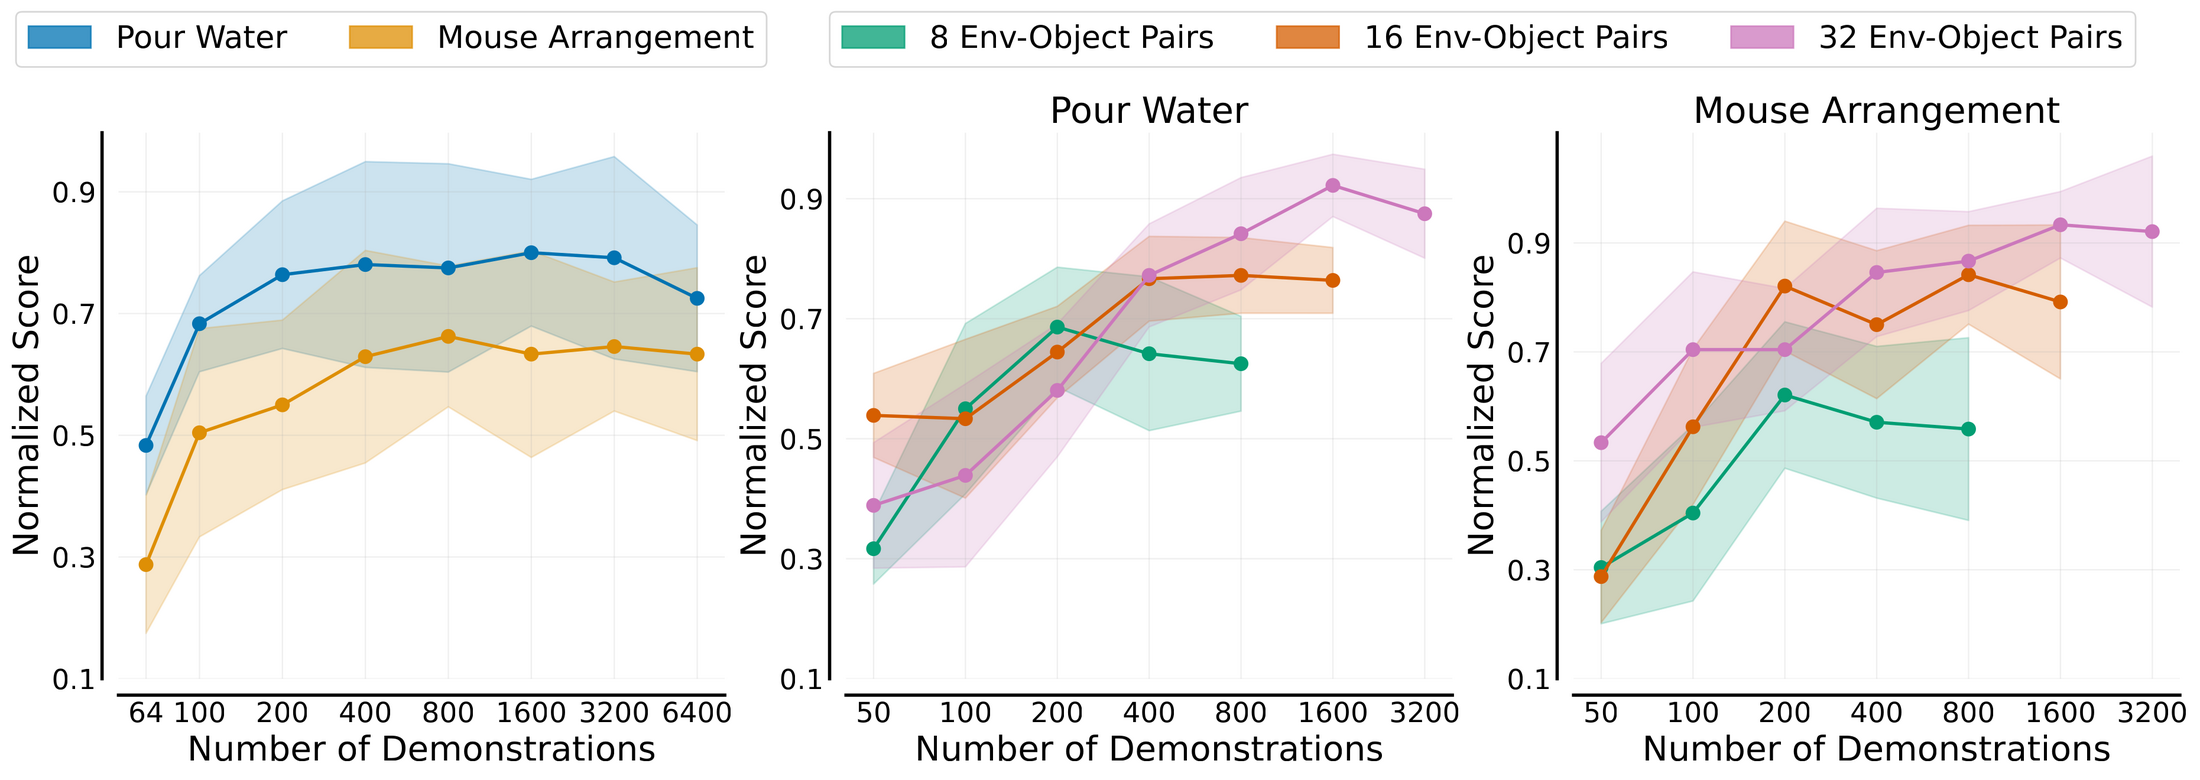
\includegraphics[keepaspectratio]{../../assets/figures/lecture09/ref/figures/fig91-data-scaling-law.png}}

}

\caption{模仿学习的数据规模律，归一化得分随示教数上升，覆盖更多环境---物体组合的策略整体更高}

\end{figure}%

\subsection{1.3
加什么数据最有用：跨本体数据的正迁移}\label{ux52a0ux4ec0ux4e48ux6570ux636eux6700ux6709ux7528ux8de8ux672cux4f53ux6570ux636eux7684ux6b63ux8fc1ux79fb}

第二个证据更有冲击力，来自 \textbf{Open X-Embodiment（OXE）}
这项联合多家机构的工作：把二十多种不同机器人、几百种技能的数据汇聚成一个大池子，用同一个模型（RT-X
系列）一起训，会发生什么？下面两张图都出自该工作。

\begin{figure}[H]

{\centering \pandocbounded{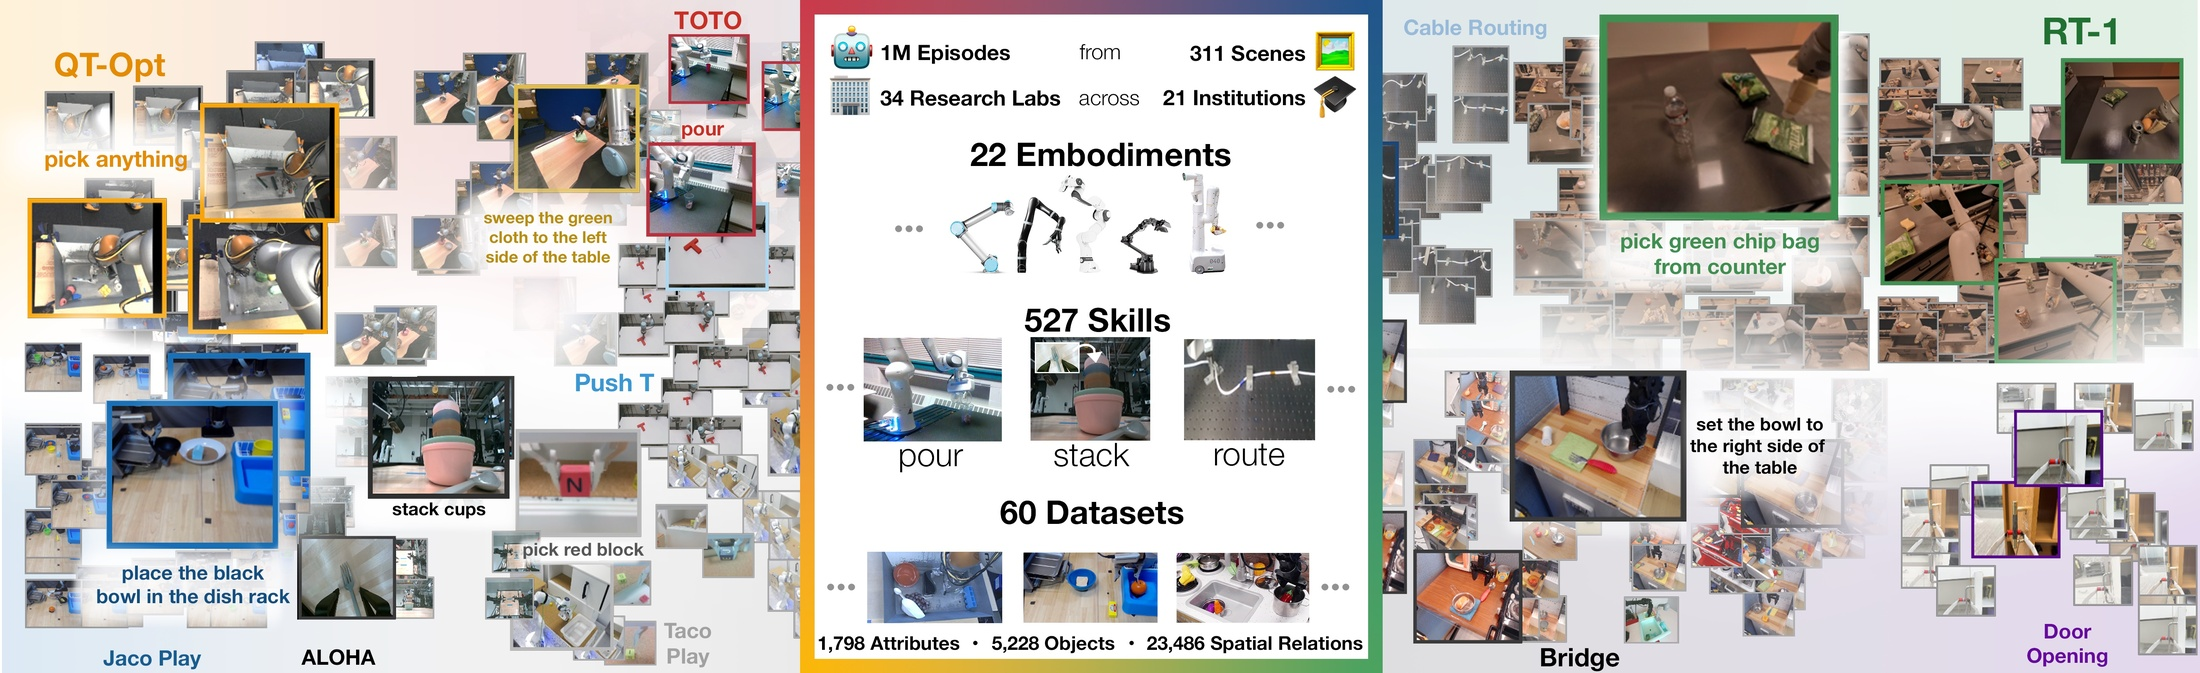
\includegraphics[keepaspectratio]{../../assets/figures/lecture09/ref/figures/fig91-oxe-dataset-montage.jpg}}

}

\caption{把二十多种机器人本体、上百万条轨迹、数百种技能汇聚成一个统一数据池}

\end{figure}%

OXE 在它那 22 种本体、RT-X
那套设置下报告的结果是\textbf{总体正迁移}：一个机器人能从其它机器人的经验里获益。在同样的网络结构下，用这个混合大池子训练，比只用单机自己的数据训练，成功率有明显抬升；更大容量的模型甚至能在分布外技能上把泛化能力提升约三倍，并涌现出原本训练集里根本没有的新行为。

\begin{figure}[H]

{\centering \pandocbounded{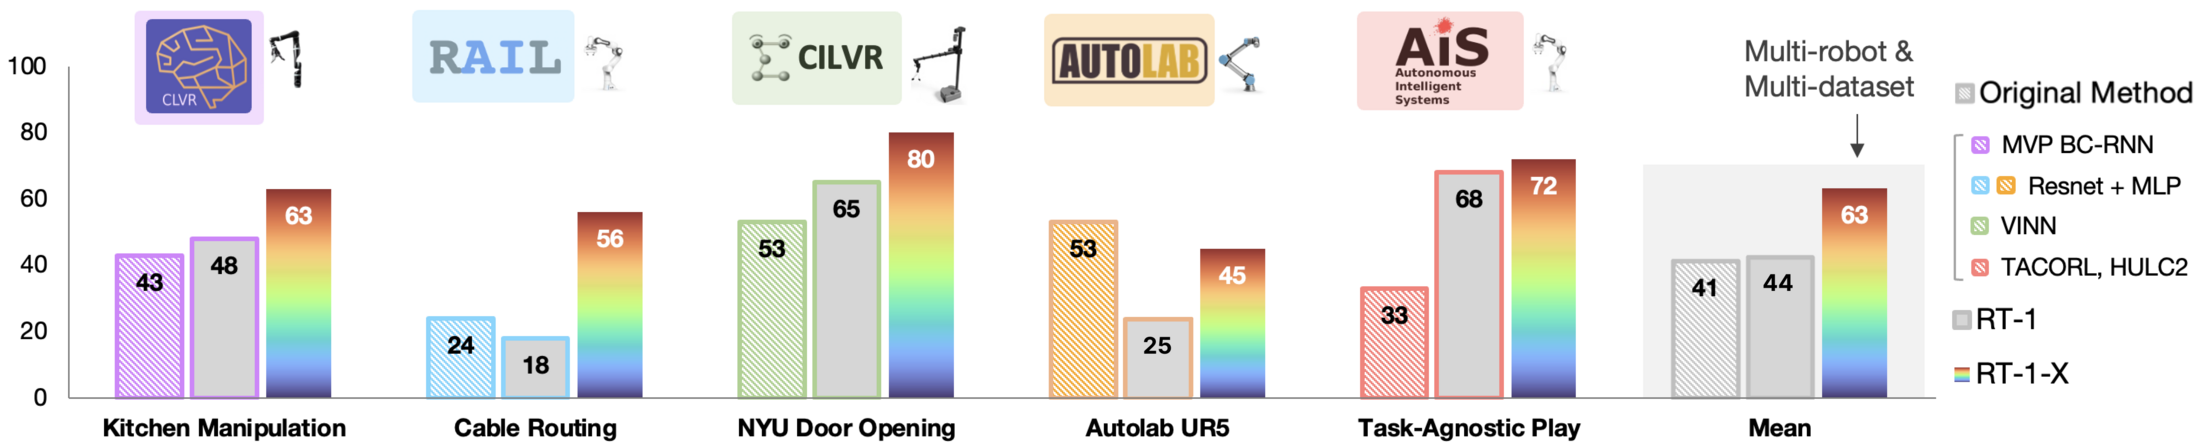
\includegraphics[keepaspectratio]{../../assets/figures/lecture09/ref/figures/fig91-rtx-positive-transfer.png}}

}

\caption{跨本体共训对比单机训练，多个数据域上成功率显著抬升，均值由 41 /
44 提升到 63}

\end{figure}%

这张图是本节最值得记住的一张：\textbf{在合适的模型与配比下，加更多、更杂的数据能把能力上限往上顶}。它把''数据决定上限''从一句口号变成了可量化的对照实验。但''总体正迁移''不等于''任意混任意数据都受益''：跨本体的收益取决于模型容量、动作表示、各数据源的采样权重和你关心的目标域------容量不够或配比失衡时，负迁移是真实存在的。所以混数据之后不能只看一个总平均分，要\textbf{把每个数据来源（每个''域''）的成绩分开报}------本体
A 的任务、本体 B
的任务、仿真的、真机的，各自算各自的成功率，再摆在一起看。总分涨了、某一个域却掉了，是混数据最常见的翻车方式；只报总分会把它盖住。

\subsection{1.4
好坏怎么界定：质量比数量更关键}\label{ux597dux574fux600eux4e48ux754cux5b9aux8d28ux91cfux6bd4ux6570ux91cfux66f4ux5173ux952e}

数据不是越多越好，\textbf{质量}同样决定上限。一项对六种离线学习算法、八个任务的系统消融发现：策略性能强烈依赖示教的质量；当数据由多人采集、质量参差不齐时，同一个算法的成功率会明显下降。也就是说，算法选择固然重要，但喂进去的数据干不干净，往往是更靠前的决定因素。

\begin{center}
\begin{tabular}{@{}>{\raggedright\arraybackslash}p{\dimexpr 0.3608\linewidth - 2\tabcolsep\relax} >{\raggedright\arraybackslash}p{\dimexpr 0.3333\linewidth - 2\tabcolsep\relax} >{\raggedright\arraybackslash}p{\dimexpr 0.3059\linewidth - 2\tabcolsep\relax}@{}}
\toprule\noalign{}
数据情形 & 现象 & 启示 \\
\midrule\noalign{}
单一熟练操作者、动作干净 & 同一算法成功率高 & 质量先于数量 \\
多人混采、质量参差 & 同一算法成功率明显下降 & 采集要控质量、要会筛 \\
盲目加量但不控质量 & 收益递减甚至变差 & ``采得多''不等于''采得好'' \\
\bottomrule\noalign{}
\end{tabular}
\end{center}

正因为如此，近年出现了把''质量''做成可度量、可筛选的方法：用影响函数去估计单条示教对策略闭环表现的因果贡献，再据此挑出真正有用的数据、剔除拖后腿的轨迹。这把''好数据''从一种感觉，变成了可以打分排序的工程量。

\subsection{1.5
多样性的''轴''：往哪个方向多样，就往哪个方向泛化}\label{ux591aux6837ux6027ux7684ux8f74ux5f80ux54eaux4e2aux65b9ux5411ux591aux6837ux5c31ux5f80ux54eaux4e2aux65b9ux5411ux6cdbux5316}

既然多样性比数量更重要，那''多样''又该往哪些方向铺？两份大规模真实数据集给了很直接的答案。

第一份是
\textbf{DROID}------一份跨七万多条轨迹、五百多个场景、几十个真实地点采了一年的数据集（下图出自该工作）。

\begin{figure}[H]

{\centering \pandocbounded{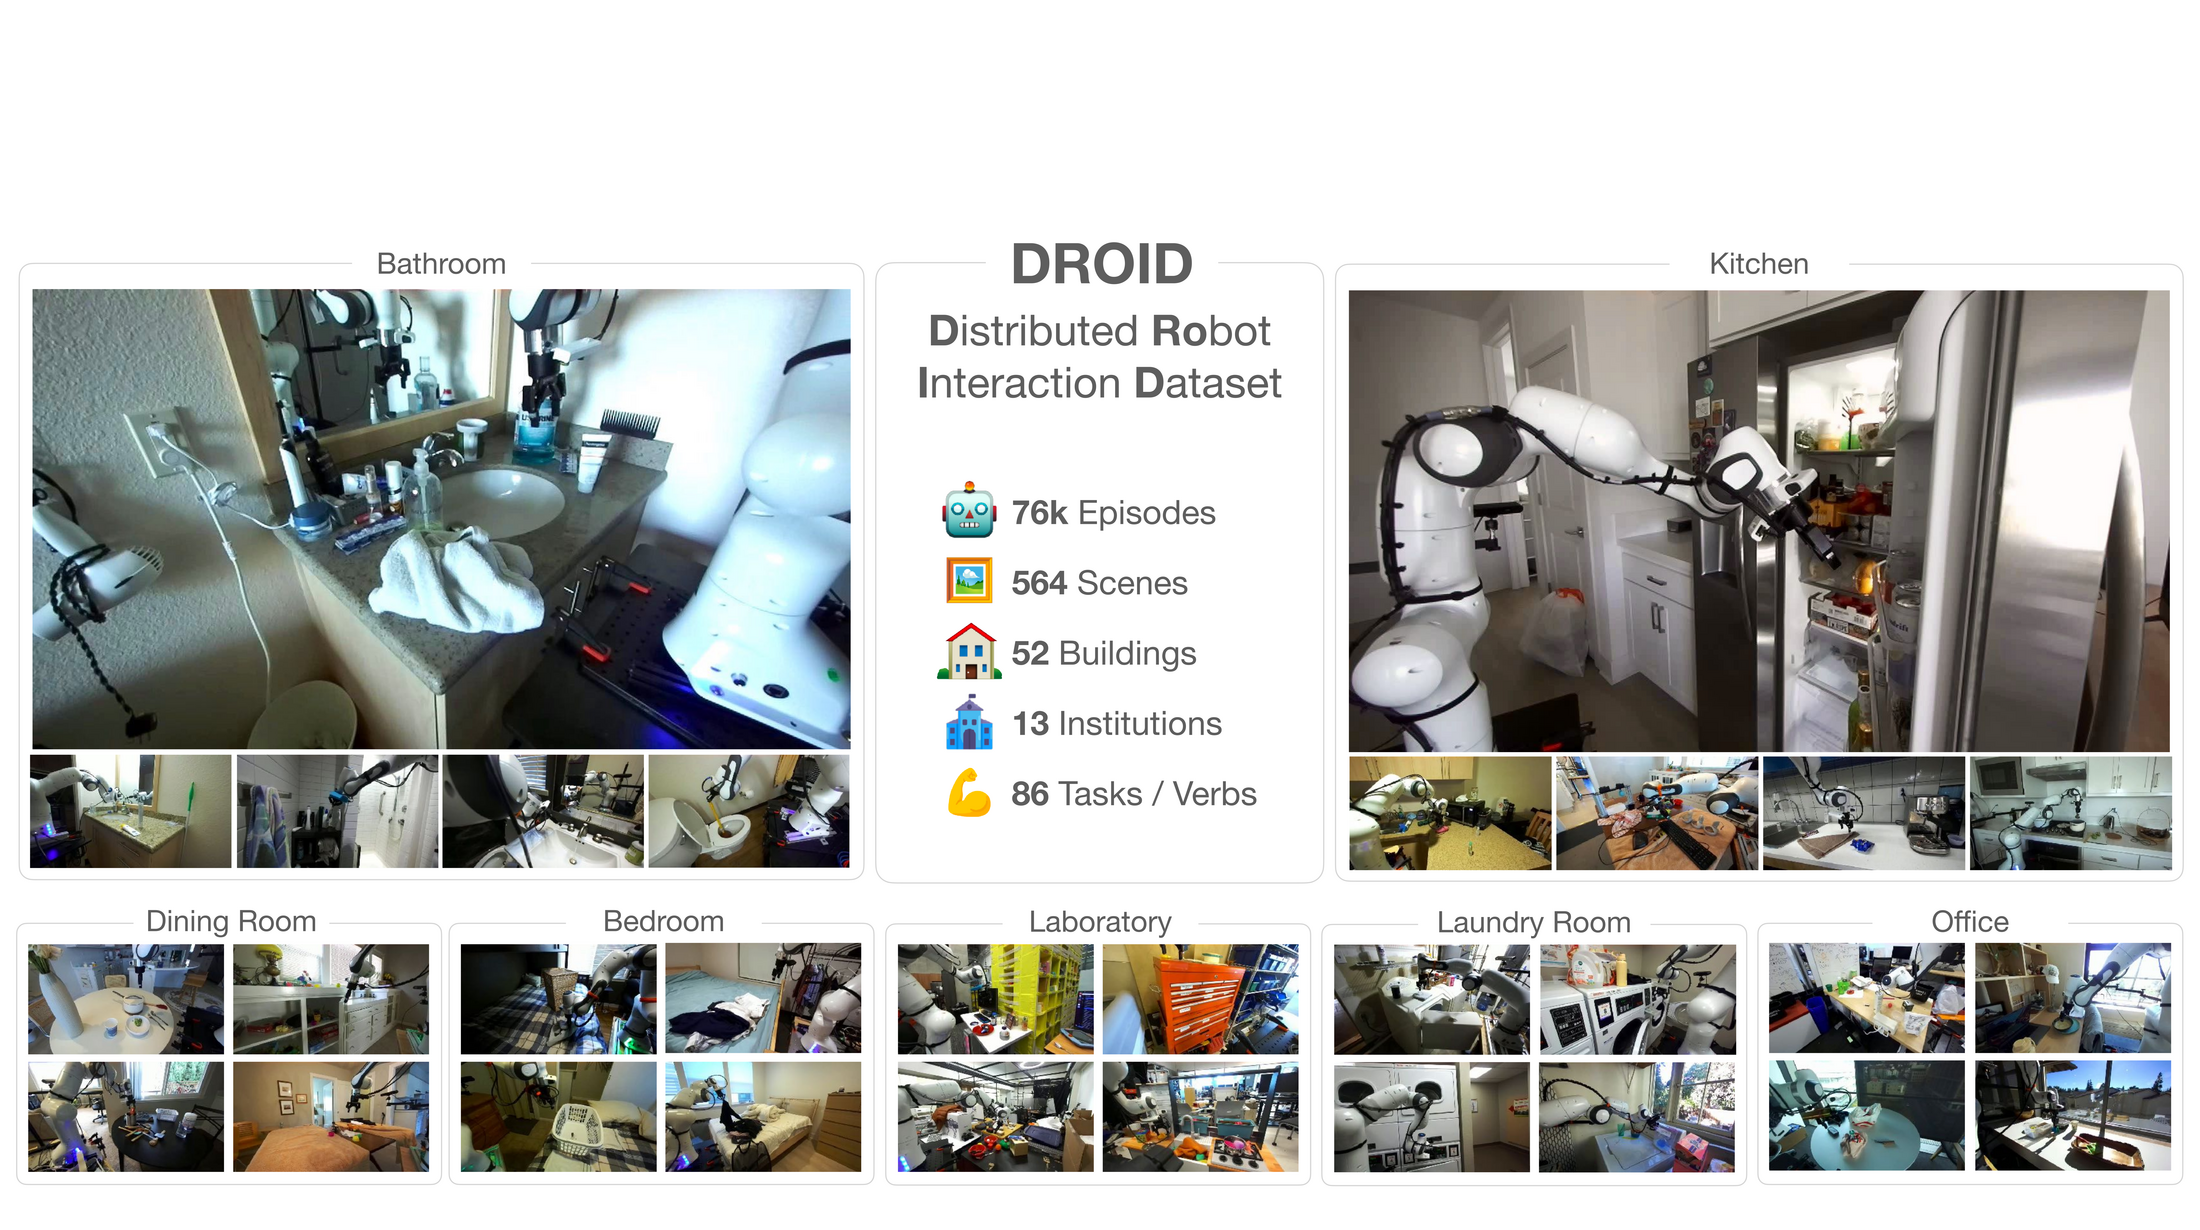
\includegraphics[keepaspectratio]{../../assets/figures/lecture09/ref/figures/fig91-droid-diversity.png}}

}

\caption{跨大量真实场景、视角与任务采集的大规模操作数据}

\end{figure}%

它显示：不同的多样性轴各自驱动\textbf{不同方向}的泛化------场景多样带来换场景的泛化，视角多样带来换相机的泛化，物体与任务多样带来换物体、换指令的泛化。这意味着采数据前要先想清楚''我要它在什么维度上泛化''，再决定在哪个轴上铺开。

第二份是 \textbf{BridgeData
V2}------一份在低成本机器人上采集的大规模多任务、多环境数据集（下图出自该工作）。

\begin{figure}[H]

{\centering \pandocbounded{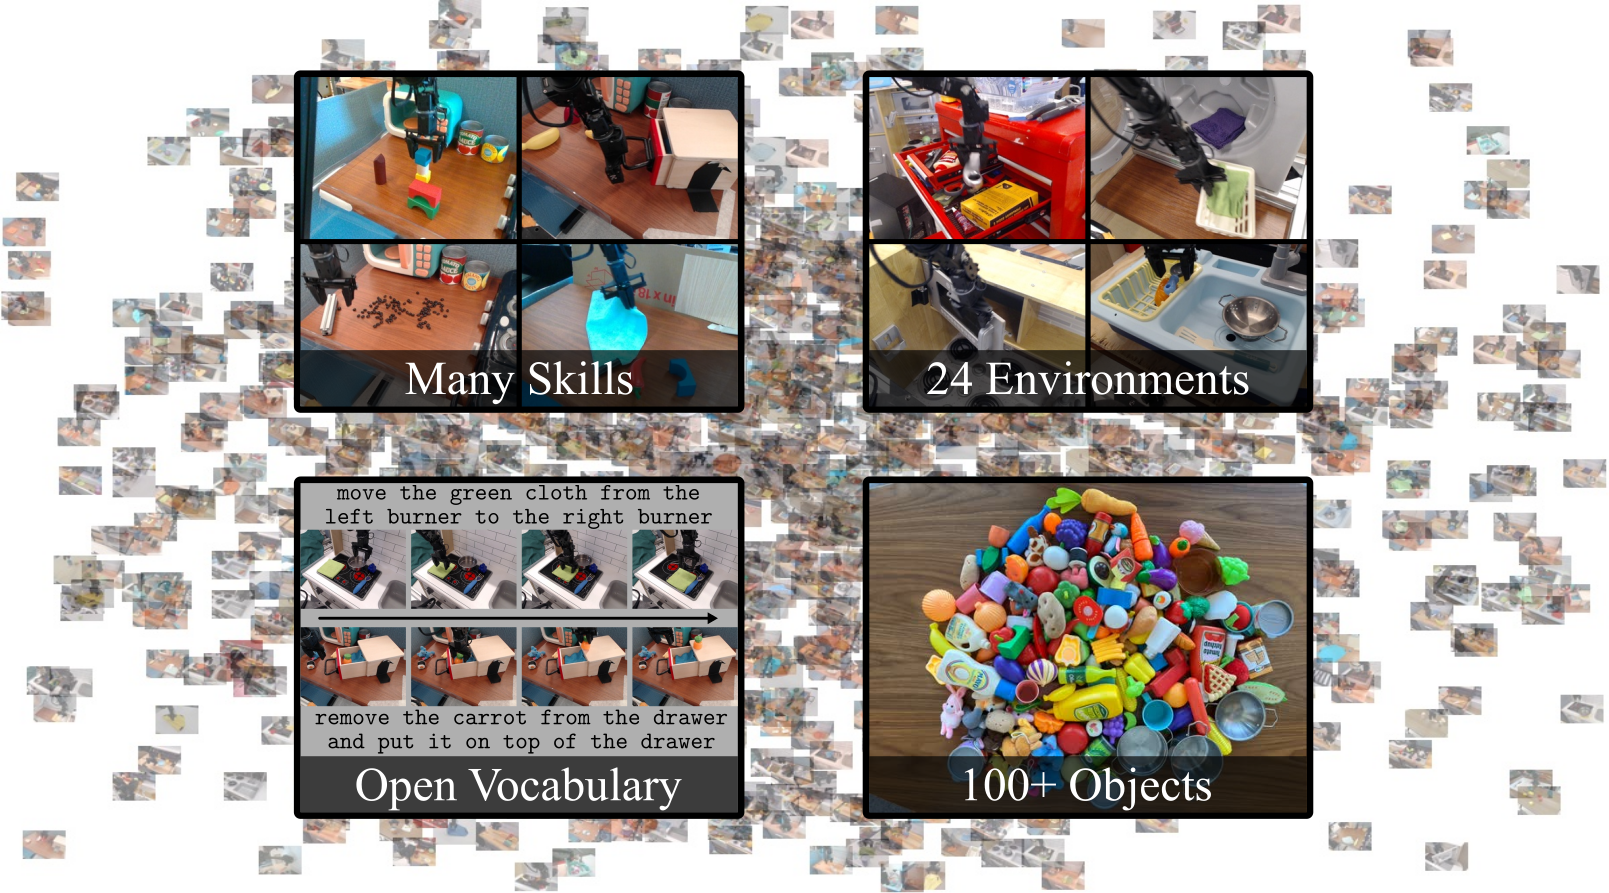
\includegraphics[keepaspectratio]{../../assets/figures/lecture09/ref/figures/fig91-bridgedata-v2.png}}

}

\caption{在低成本机器人上采集的大规模多任务、多环境数据集}

\end{figure}%

它印证了同一点：足够宽的任务与环境覆盖，能让学到的技能跨环境、甚至跨实验室迁移。

需要留一句边界：以上都是\textbf{在这些论文覆盖的任务、物体类别与采集协议范围内}观察到的经验趋势，不是保证。跨实验室还要受硬件型号、相机配置、控制接口和操作员习惯的影响；一旦超出原本的本体、任务或传感器分布，多样性带来的泛化就得重新验证，不能直接外推。

\subsection{1.6
小结：数据决定上限}\label{ux5c0fux7ed3ux6570ux636eux51b3ux5b9aux4e0aux9650}

把这一节收一下，``数据决定上限''不是口号，而是一串互相印证的证据：

\begin{center}
\begin{tabular}{@{}>{\raggedright\arraybackslash}p{\dimexpr 0.2188\linewidth - 2\tabcolsep\relax} >{\raggedright\arraybackslash}p{\dimexpr 0.7500\linewidth - 2\tabcolsep\relax}@{}}
\toprule\noalign{}
证据 & 一句话结论 \\
\midrule\noalign{}
数据规模律 & 加数据，泛化大致按幂律上升 \\
跨本体正迁移 & 加更杂的数据，能力直接抬升、涌现新技能 \\
质量消融 & 同一算法，好数据远胜坏数据 \\
多样性轴 & 在覆盖范围内，往哪个方向多样，就往哪个方向泛化 \\
\bottomrule\noalign{}
\end{tabular}
\end{center}

当然，数据也不是万能钥匙------光有数据和大模型仍不够，怎么把海量无结构的人类行为高效转成机器人能用的监督信号，本身就是一个开放问题。但这恰恰把话题自然带到下一节：既然好数据这么关键，\textbf{到底怎么把它采出来}。

\section{2
遥操作采集方法概述}\label{ux9065ux64cdux4f5cux91c7ux96c6ux65b9ux6cd5ux6982ux8ff0}

要采到能训练的操作数据，核心动作是\textbf{遥操作}：让人去''驱动''机器人完成任务，同时把每一帧的观测和动作记录下来。问题是，``让人驱动机器人''有非常多种做法，成本、便携性、数据质量各不相同。这一节先把它们铺成一张分类地图。

\subsection{2.1
一张分类地图：四大类与一条权衡轴}\label{ux4e00ux5f20ux5206ux7c7bux5730ux56feux56dbux5927ux7c7bux4e0eux4e00ux6761ux6743ux8861ux8f74}

按''机器人和人体在数据回路里占多少''，可以把采集方法从重到轻分成四大类：真机数据、人类代理数据、通用接口遥操作、无机器人数据。

一条权衡贯穿整张地图：

\begin{center}
\begin{tabular}{@{}>{\raggedright\arraybackslash}p{\dimexpr 0.1356\linewidth - 2\tabcolsep\relax} >{\raggedright\arraybackslash}p{\dimexpr 0.1952\linewidth - 2\tabcolsep\relax} >{\raggedright\arraybackslash}p{\dimexpr 0.1207\linewidth - 2\tabcolsep\relax} >{\raggedright\arraybackslash}p{\dimexpr 0.1431\linewidth - 2\tabcolsep\relax} >{\raggedright\arraybackslash}p{\dimexpr 0.1803\linewidth - 2\tabcolsep\relax} >{\raggedright\arraybackslash}p{\dimexpr 0.2251\linewidth - 2\tabcolsep\relax}@{}}
\toprule\noalign{}
大类 & 机器人是否在回路 & 轨迹可执行性 & 便携 / 可规模化 & 是否需重定向或后处理 & 典型代表 \\
\midrule\noalign{}
真机数据 & 在回路 & 高，物理可行 & 低 & 否 & 主从臂、原机示教 \\
人类代理数据 & 不在回路，人戴或持设备 & 中 & 高 & 是 & 手持夹爪、数据手套 \\
通用接口遥操作 & 在回路，靠接口驱动 & 中高 & 中 & 部分 & 手柄、VR/AR \\
无机器人数据 & 完全不在回路 & 低，需转化 & 极高 & 是，强转化 & 第一视角视频、世界模型生成 \\
\bottomrule\noalign{}
\end{tabular}
\end{center}

简单说：\textbf{机器人越在回路里，采到的轨迹越能直接执行，但越贵越不便携；机器人越不在回路，采集越轻便越能规模化，但越需要后处理或重定向才能变成机器人能用的动作}。下面逐类展开。

\subsection{2.2
真机数据：机器人在回路}\label{ux771fux673aux6570ux636eux673aux5668ux4ebaux5728ux56deux8def}

\subsubsection{2.2.1 原机示教}\label{ux539fux673aux793aux6559}

最直接的做法是人手把手地拖动真机或灵巧手完成任务，让传感器把轨迹记录下来。它的天然优势是采集时就带上了真实的接触与触觉信息。下图来自
\textbf{KineDex} 这项工作。

\begin{figure}[H]

{\centering \pandocbounded{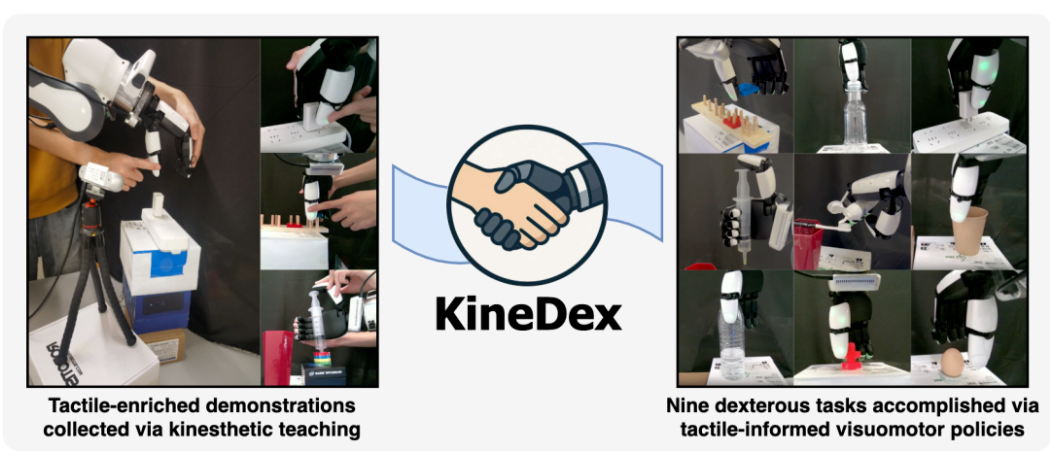
\includegraphics[keepaspectratio]{../../assets/figures/lecture09/ref/figures/fig92-kinedex.png}}

}

\caption{人手把手带动灵巧手做示教，采集带触觉与接触信息的高保真示教}

\end{figure}%

面向柔顺的软体手时，这种拖动示教更显自然，柔顺性本身反而成了示教的便利------下图来自
\textbf{KineSoft}。

\begin{figure}[H]

{\centering \pandocbounded{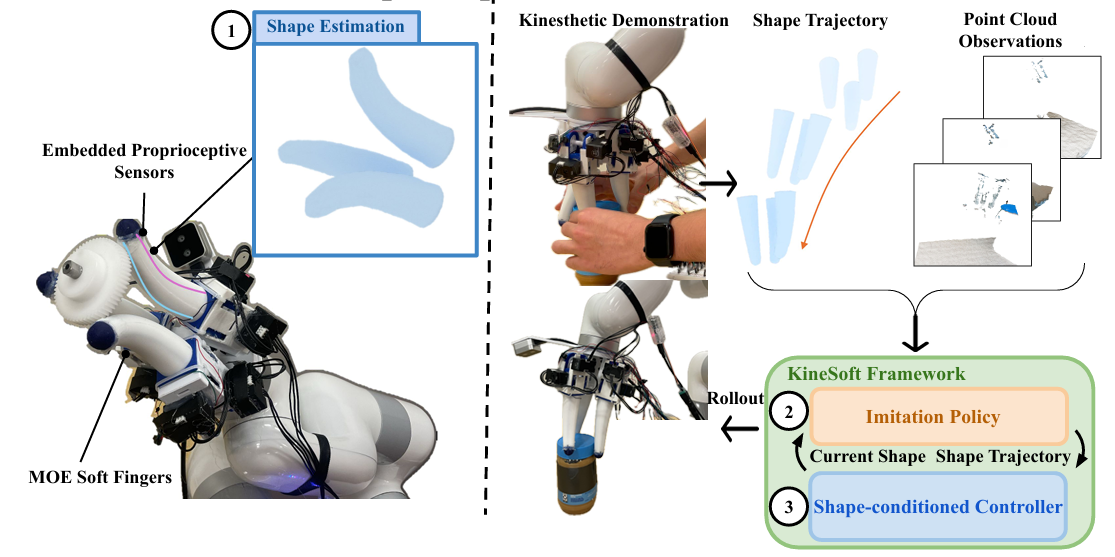
\includegraphics[keepaspectratio]{../../assets/figures/lecture09/ref/figures/fig92-kinesoft.png}}

}

\caption{面向软体手的拖动示教，把柔顺性当作示教的便利}

\end{figure}%

\subsubsection{2.2.2
主从臂（同构）}\label{ux4e3bux4eceux81c2ux540cux6784}

更常见的是主从臂：操作者驱动一只''主臂''，机器人''从臂''实时跟随。当主臂与从臂机械结构相同（同构）时，关节映射变得很简单------省掉了跨本体重定向那一层，采到的轨迹落在从臂自己的可达空间里，对模仿学习最友好。但''结构相同''不等于''数值可以直接搬''：关节顺序、正方向、零位、量程、减速比、限位、安装姿态都得先对齐，标定没做准，映射就是错的；从臂还有跟踪误差、碰撞和接触约束，主臂摆到的姿态它未必真到得了。下面两张分别是松灵
\textbf{PIKA} 方案与本课实物实验要用的低成本代表 \textbf{SO-101}。

\begin{figure}[H]

{\centering \pandocbounded{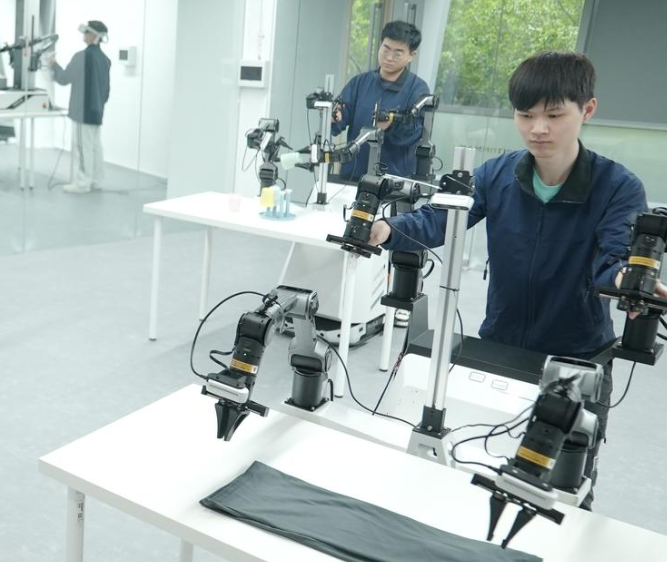
\includegraphics[keepaspectratio]{../../assets/figures/lecture09/ref/figures/fig92-pika.png}}

}

\caption{松灵 PIKA 主从采集方案}

\end{figure}%

\begin{figure}[H]

{\centering \pandocbounded{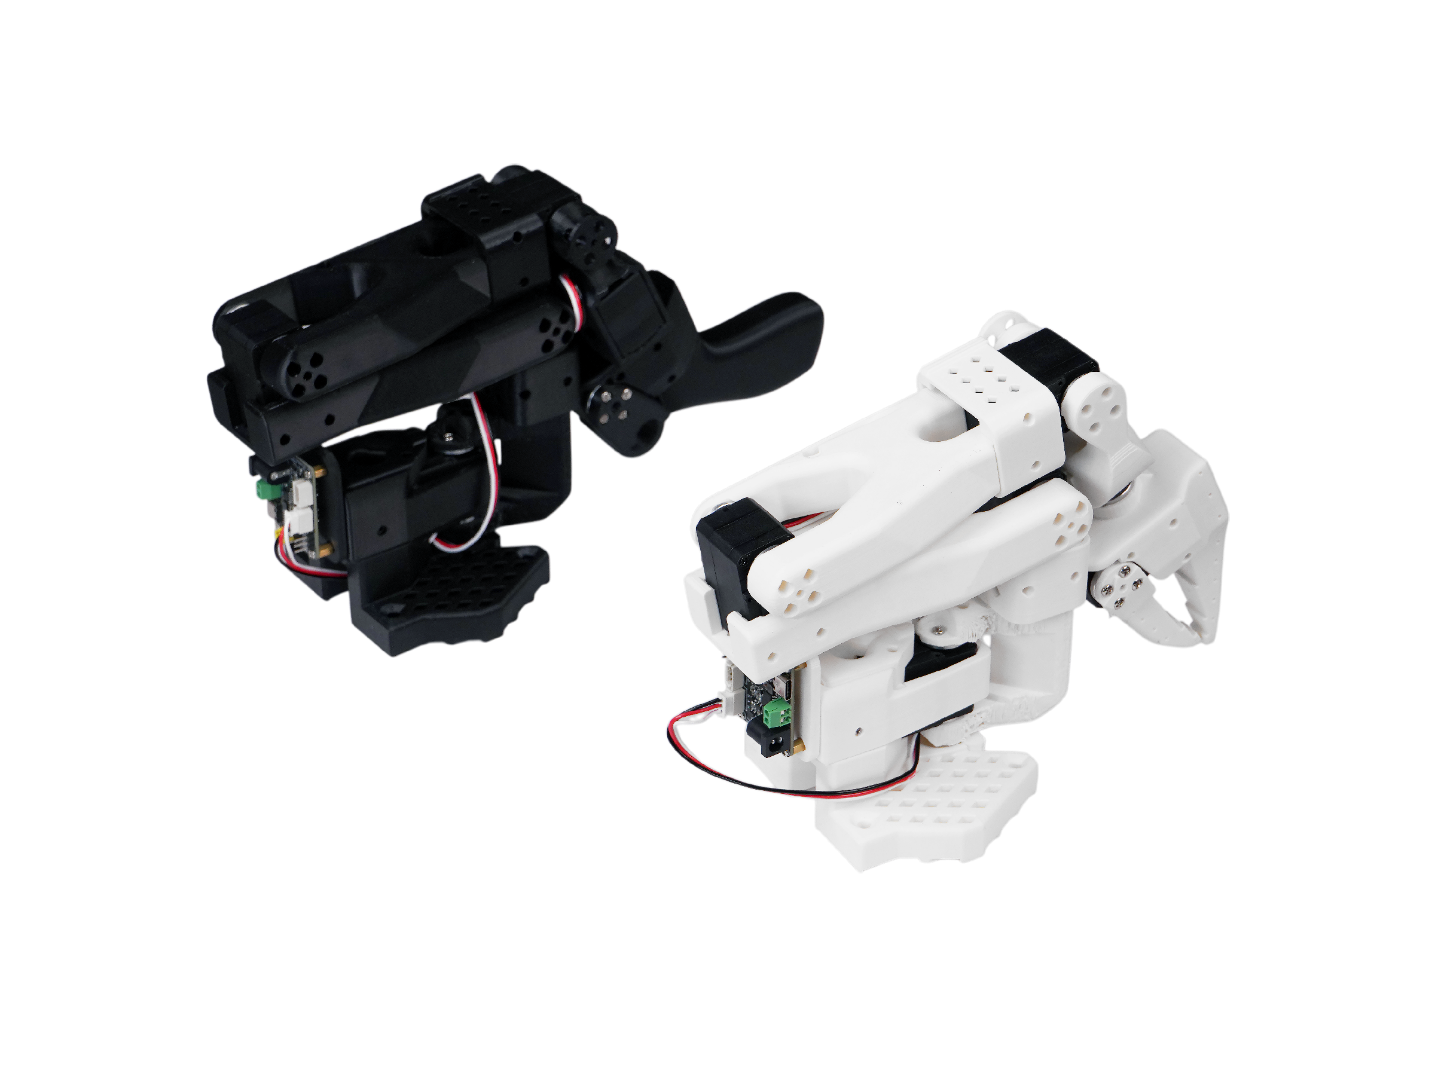
\includegraphics[keepaspectratio]{../../assets/figures/lecture09/ref/figures/fig92-so101-leader-follower.png}}

}

\caption{SO-101 主从臂，本课实物实验采集平台}

\end{figure}%

把主从臂装上移动底座，就能采''边走边操作''的全身数据；这一路线（\textbf{Mobile
ALOHA}）只用几十条示教就能学会相当长的家务任务，下图即出自该工作。

\begin{figure}[H]

{\centering \pandocbounded{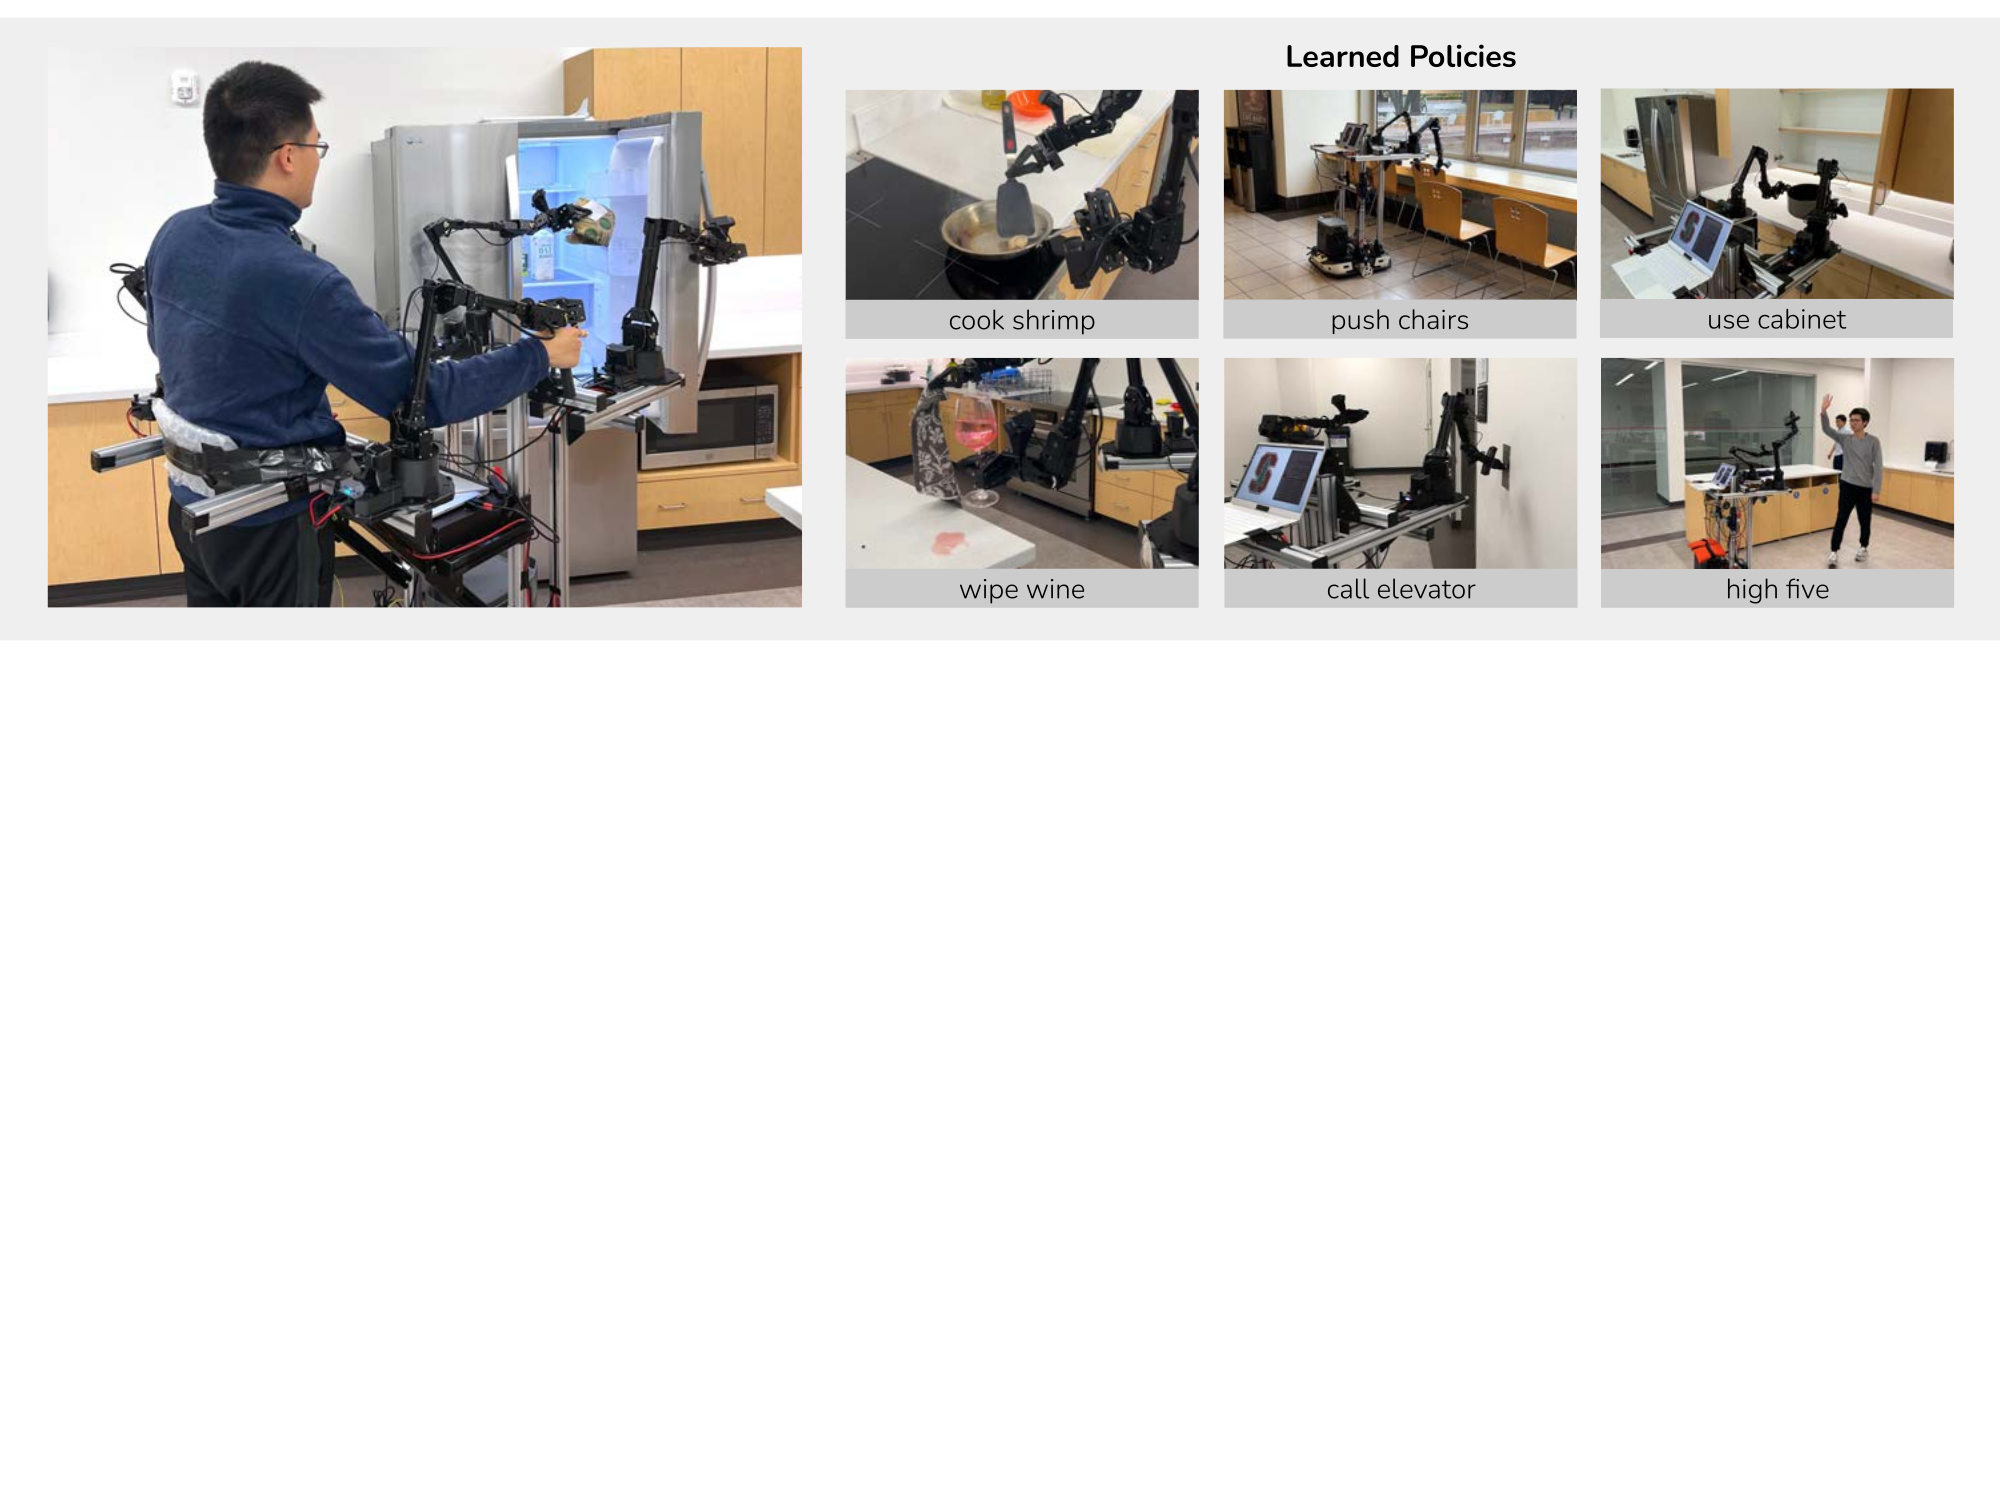
\includegraphics[keepaspectratio]{../../assets/figures/lecture09/ref/figures/fig92-mobile-aloha.png}}

}

\caption{在双臂主从基础上加移动底座，采集全身移动操作数据}

\end{figure}%

主从跟随还有一个容易被忽略的约定：从臂\textbf{怎么}跟随主臂。一种是\textbf{绝对跟踪}------从臂直接去主臂当前的绝对姿态，主臂摆成什么姿势、从臂就到达同一个姿势，跟从臂开机时停在哪无关，前提是主从标定的零点对齐。另一种是\textbf{相对（锚定）跟踪}------接通的第一帧记下''从臂当前姿态减主臂姿态''这个差，之后每帧的从臂目标就是''主臂姿态加上这个差''，相当于从臂从自己此刻的位置出发，复现主臂的\textbf{位移}。

两种口径都能用，锚定跟踪本身不是错------它不要求零点严格对齐、接通瞬间从臂也不会突然跳过去，用起来省事。真正会出问题的是\textbf{口径没被固定、偏置没被记下来}：锚定量每次开机都不同，如果不存下来，同一份数据集里不同
episode
的动作标签其实对应着不同的偏置，训练出的模型部署时就容易和环境''说的不是同一种话''（上一讲
3.3 的口径坑）。所以规矩是：口径（absolute 还是
anchored）写死在采集配置里、标定与锚点一起存进数据集、训练端和部署端用同一套解释。

还有一个概念要分清：\textbf{主臂读数、下发给从臂的目标，都是''命令''（动作标签）；从臂真实到达的姿态得从它自己的编码器读}。跟踪误差、负载、接触都会让两者不等。所以采集时最好三样分开记：\texttt{leader\ command}（主臂读数）、\texttt{follower\ target}（下发目标）、\texttt{follower\ measured\ state}（从臂实测状态）。把命令当成实际轨迹，是数据侧一个很隐蔽的错。

\subsubsection{2.2.3
主从臂（异构）}\label{ux4e3bux4eceux81c2ux5f02ux6784}

如果主臂和从臂结构不同（异构），就不能直接映射，需要标定、滤波、插值这一串处理把主臂指令对齐到目标机械臂。它的价值在于通用------一套低成本主端可以适配各种商用机械臂，下图来自
\textbf{U-Arm} 这套超低成本通用遥操接口。

\begin{figure}[H]

{\centering \pandocbounded{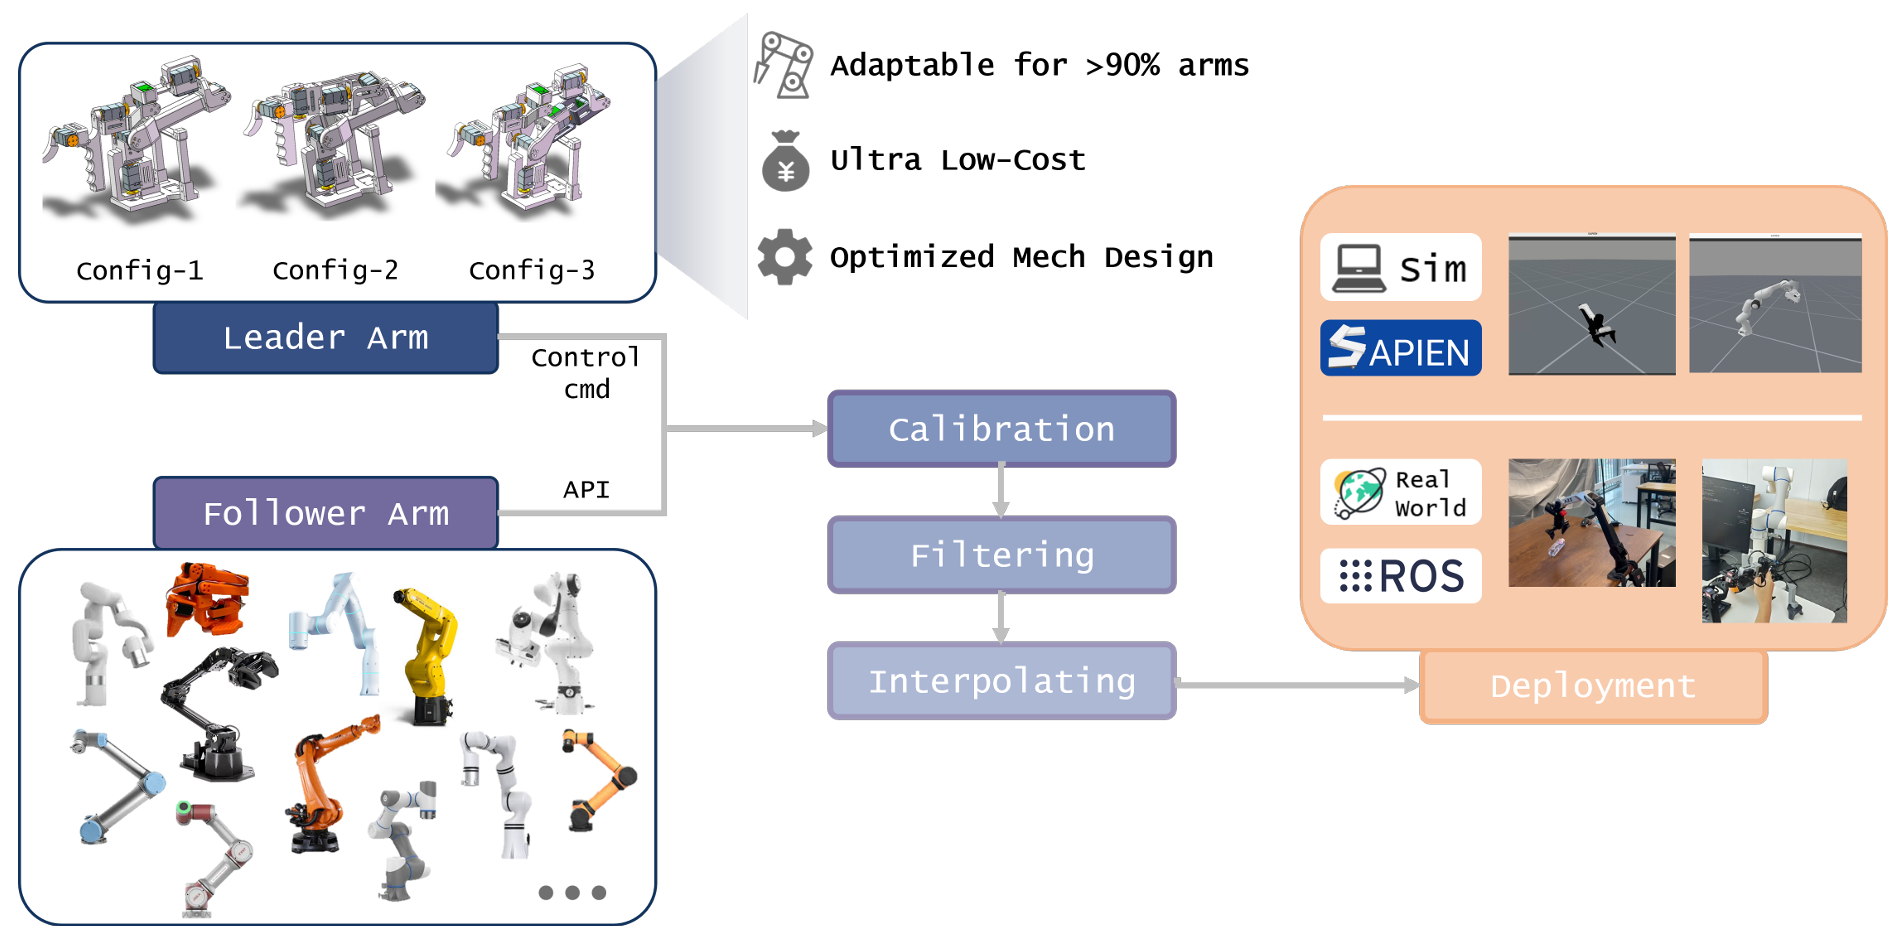
\includegraphics[keepaspectratio]{../../assets/figures/lecture09/ref/figures/fig92-uarm-hetero.png}}

}

\caption{异构主从采集，经标定、滤波、插值适配各种商用机械臂}

\end{figure}%

\subsubsection{2.2.4
移动操作整机遥操}\label{ux79fbux52a8ux64cdux4f5cux6574ux673aux9065ux64cd}

当目标是一台带底盘、带双臂的移动操作整机时，往往需要一个能统一多种输入的遥操作接口，把相机、VR、键鼠、手柄等任意组合起来同时驱动底盘和手臂。下图来自模块化遥操系统
\textbf{TeleMoMa}。

\begin{figure}[H]

{\centering \pandocbounded{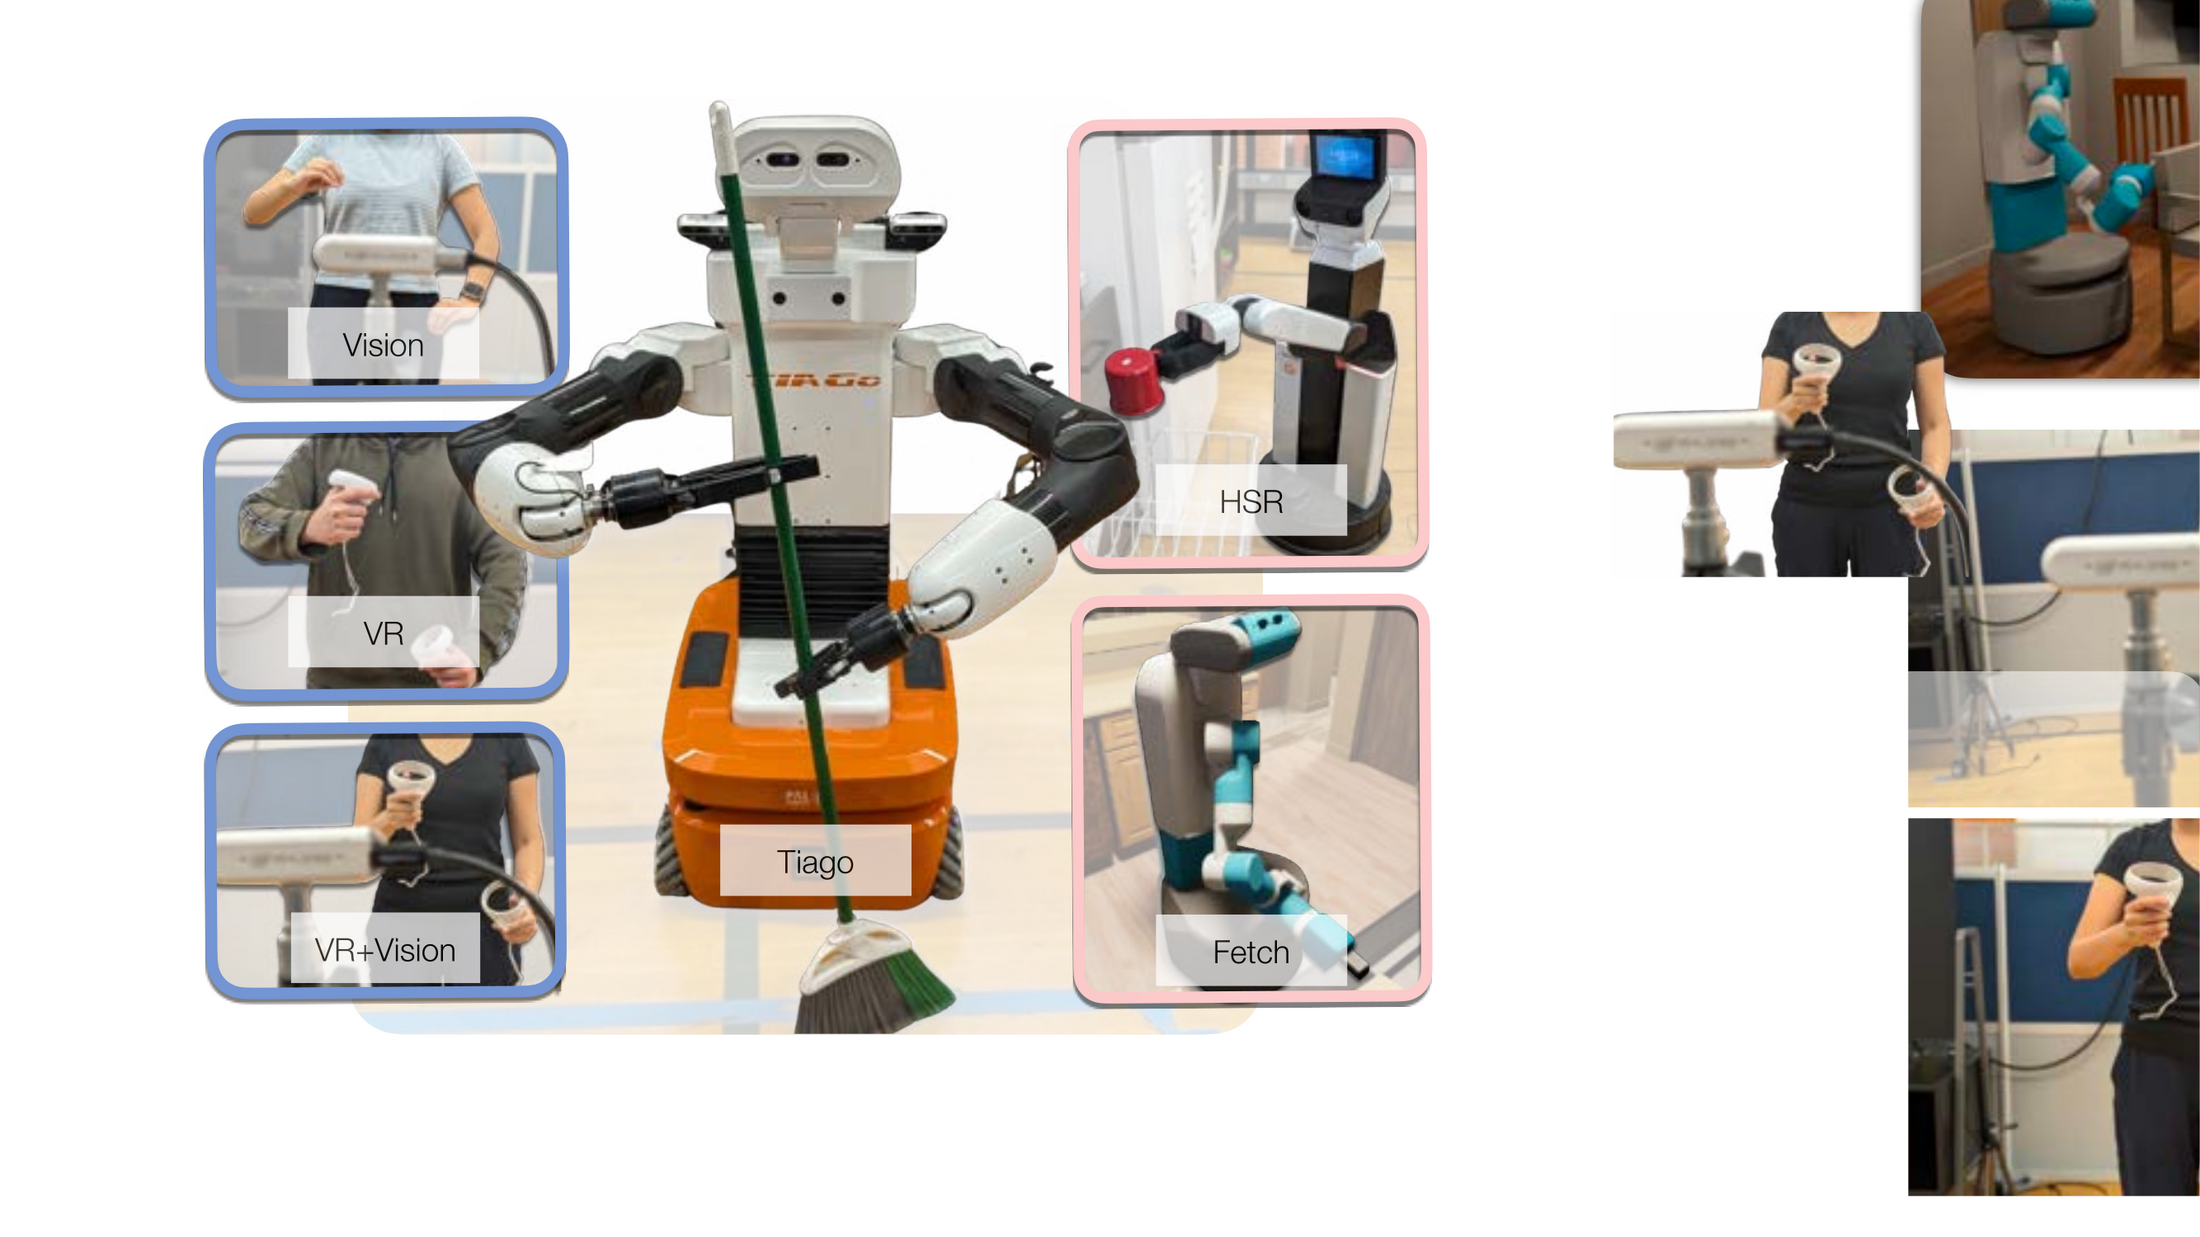
\includegraphics[keepaspectratio]{../../assets/figures/lecture09/ref/figures/fig92-telemoma.png}}

}

\caption{模块化的移动操作整机遥操，统一多种人机输入}

\end{figure}%

\subsection{2.3
人类代理数据：人戴或持设备}\label{ux4ebaux7c7bux4ee3ux7406ux6570ux636eux4ebaux6234ux6216ux6301ux8bbeux5907}

这一类不让机器人进回路，而是让人戴上或拿起一个''代理设备''去做任务，事后再把人的动作重定向到机器人。好处是轻、快、能在真实场景里大规模采，代价是采到的轨迹可能撞上机器人的运动学奇异、超出工作空间或精度不足，需要后处理。

\subsubsection{2.3.1
末端执行器代理（手持）}\label{ux672bux7aefux6267ux884cux5668ux4ee3ux7406ux624bux6301}

最典型的是
\textbf{UMI}------手持一个夹爪加广角相机，直接记录末端执行器的运动轨迹，整套装置与机器人解耦、可以带到任何场景里采，下图出自该工作。

\begin{figure}[H]

{\centering \pandocbounded{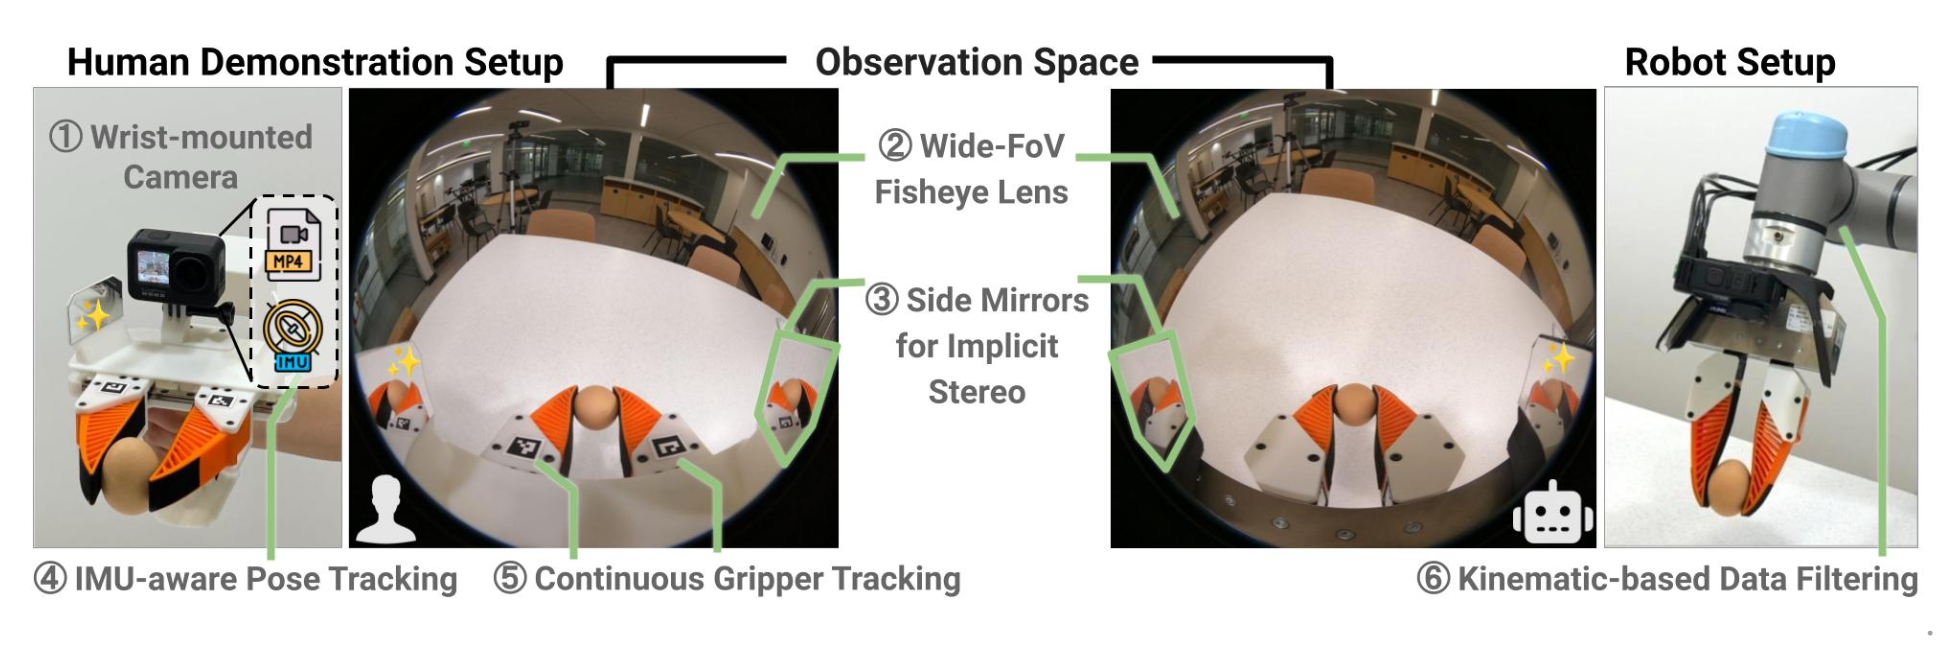
\includegraphics[keepaspectratio]{../../assets/figures/lecture09/ref/figures/fig92-umi.png}}

}

\caption{手持平行夹爪加广角相机，记录末端轨迹并做运动学过滤}

\end{figure}%

把其中复杂的视觉惯性里程计换成现成的跟踪模块，可以在保住精度的同时大幅降低部署复杂度------这是
\textbf{FastUMI} 的思路。

\begin{figure}[H]

{\centering \pandocbounded{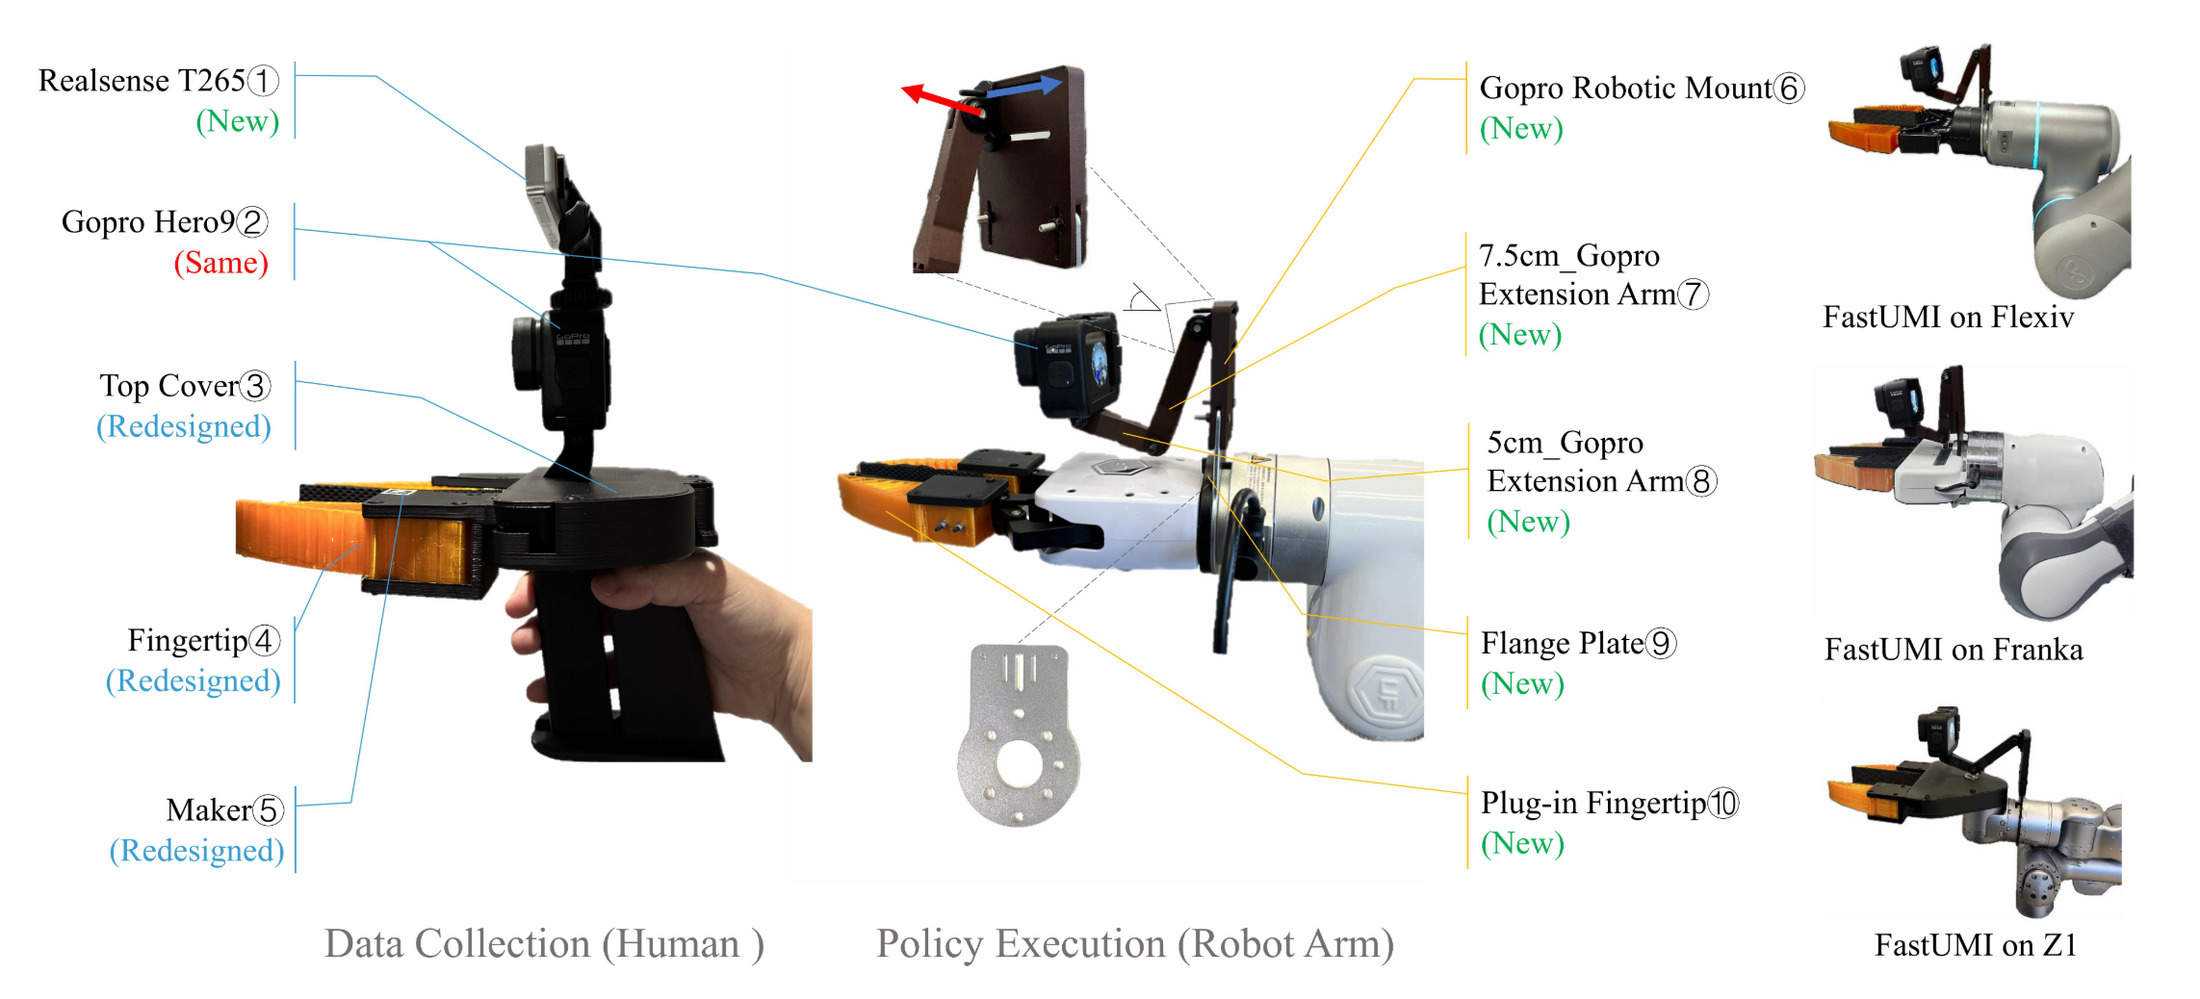
\includegraphics[keepaspectratio]{../../assets/figures/lecture09/ref/figures/fig92-fastumi.png}}

}

\caption{用现成跟踪模块替换复杂视觉惯性里程计，降低部署门槛}

\end{figure}%

视觉式的方案还能进一步做到跨机械臂、跨灵巧手、跨相机配置的通用遥操，下图来自
\textbf{AnyTeleop}。

\begin{figure}[H]

{\centering \pandocbounded{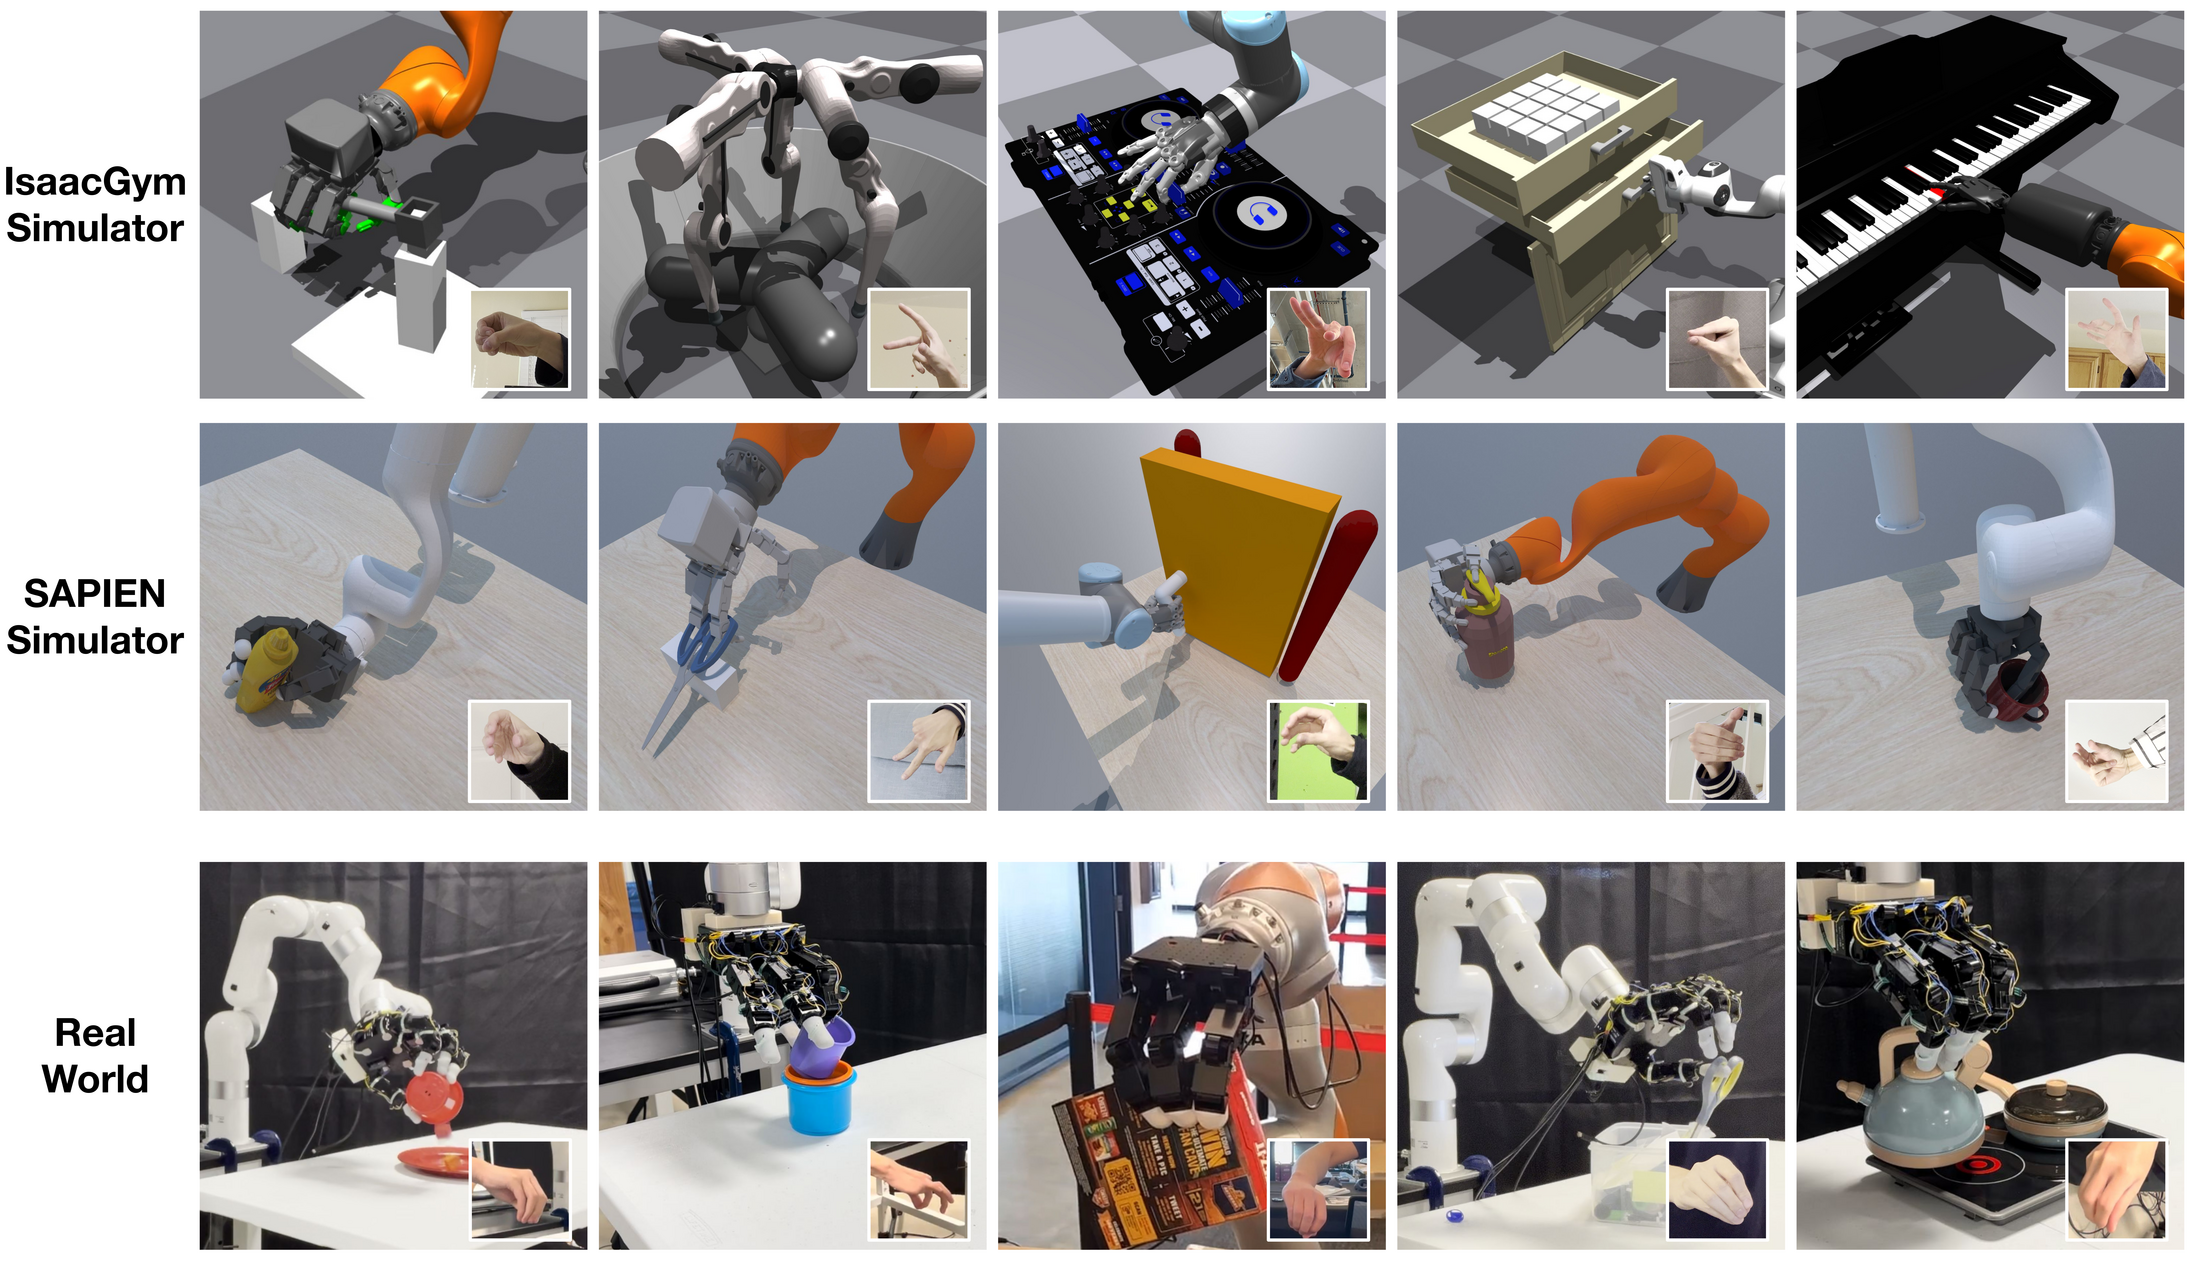
\includegraphics[keepaspectratio]{../../assets/figures/lecture09/ref/figures/fig92-anyteleop.png}}

}

\caption{跨臂、跨手、跨相机配置的通用视觉式灵巧遥操}

\end{figure}%

\subsubsection{2.3.2
增强现实反馈采集}\label{ux589eux5f3aux73b0ux5b9eux53cdux9988ux91c7ux96c6}

手持代理的一个痛点是：人采得很顺，机器人却未必执行得了。一个改进思路（\textbf{ARCap}）是在采集时给操作者叠加实时的增强现实提示------把机器人的可达范围、工作空间、虚拟手臂预览实时显示出来，引导人把示教约束在机器人能执行的范围内，从源头提高数据可用率，下图出自该工作。

\begin{figure}[H]

{\centering \pandocbounded{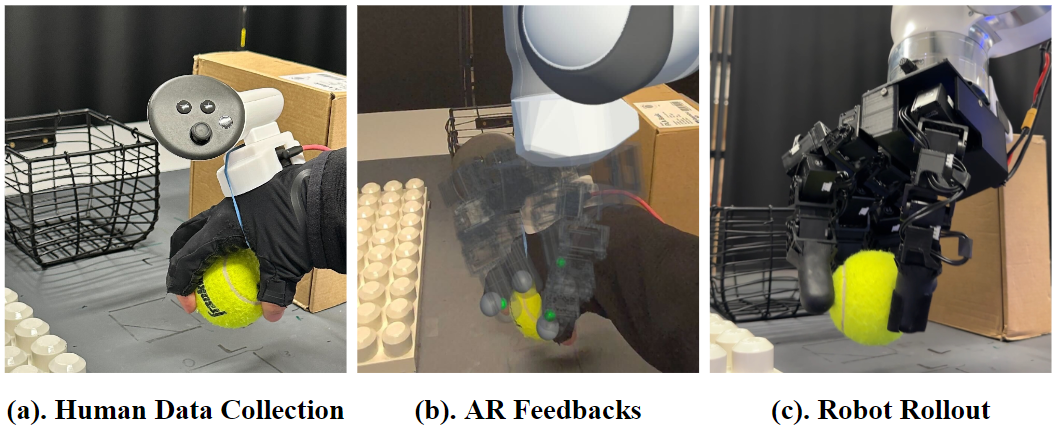
\includegraphics[keepaspectratio]{../../assets/figures/lecture09/ref/figures/fig92-arcap.png}}

}

\caption{在增强现实反馈下采集高质量、可被机器人执行的人类示教}

\end{figure}%

\subsubsection{2.3.3
穿戴设备代理}\label{ux7a7fux6234ux8bbeux5907ux4ee3ux7406}

把代理设备做成可穿戴的数据手套、外骨骼或背负式装置，就能在采动作的同时采到力与触觉反馈。下面两张分别来自低成本开源数据手套
\textbf{DOGlove} 与背负式人形双臂遥操设备 \textbf{U-Arm Humanoid}。

\begin{figure}[H]

{\centering \pandocbounded{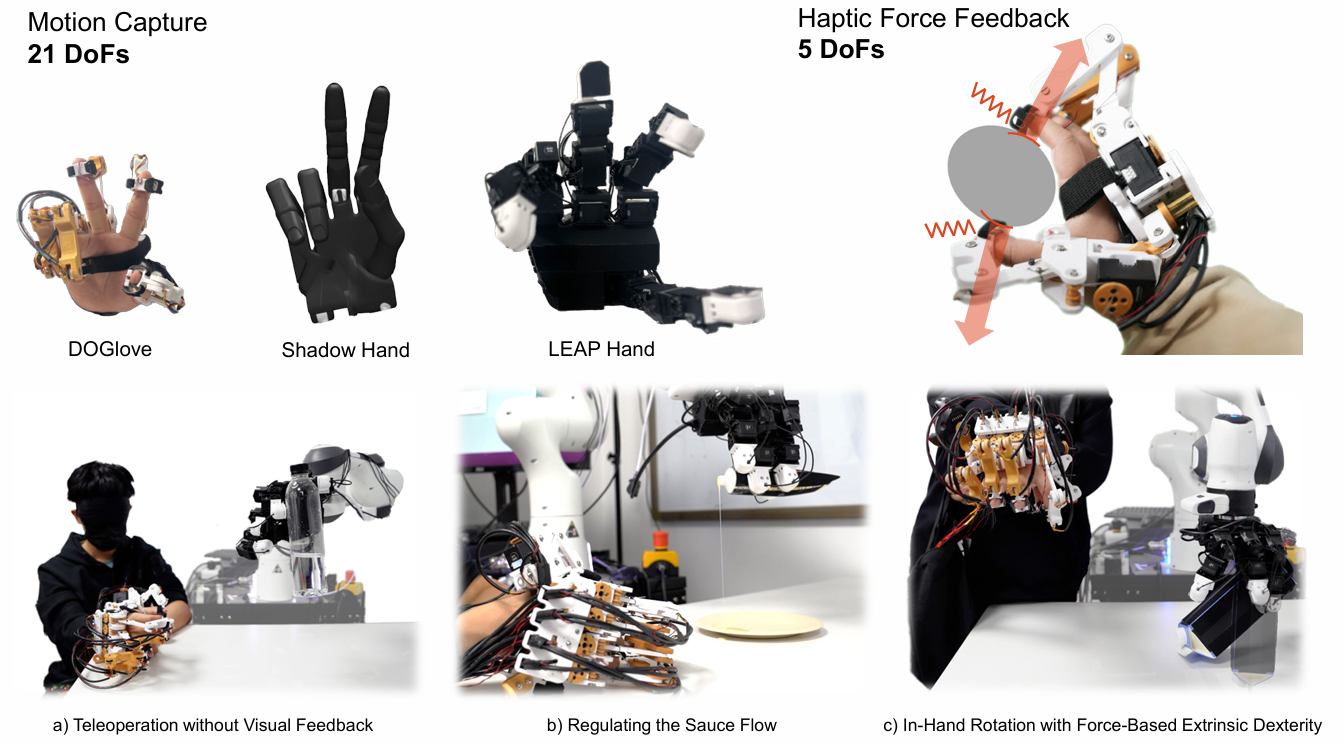
\includegraphics[keepaspectratio]{../../assets/figures/lecture09/ref/figures/fig92-doglove.png}}

}

\caption{低成本开源数据手套，同时采集多自由度动作与力 / 触觉反馈}

\end{figure}%

\begin{figure}[H]

{\centering \pandocbounded{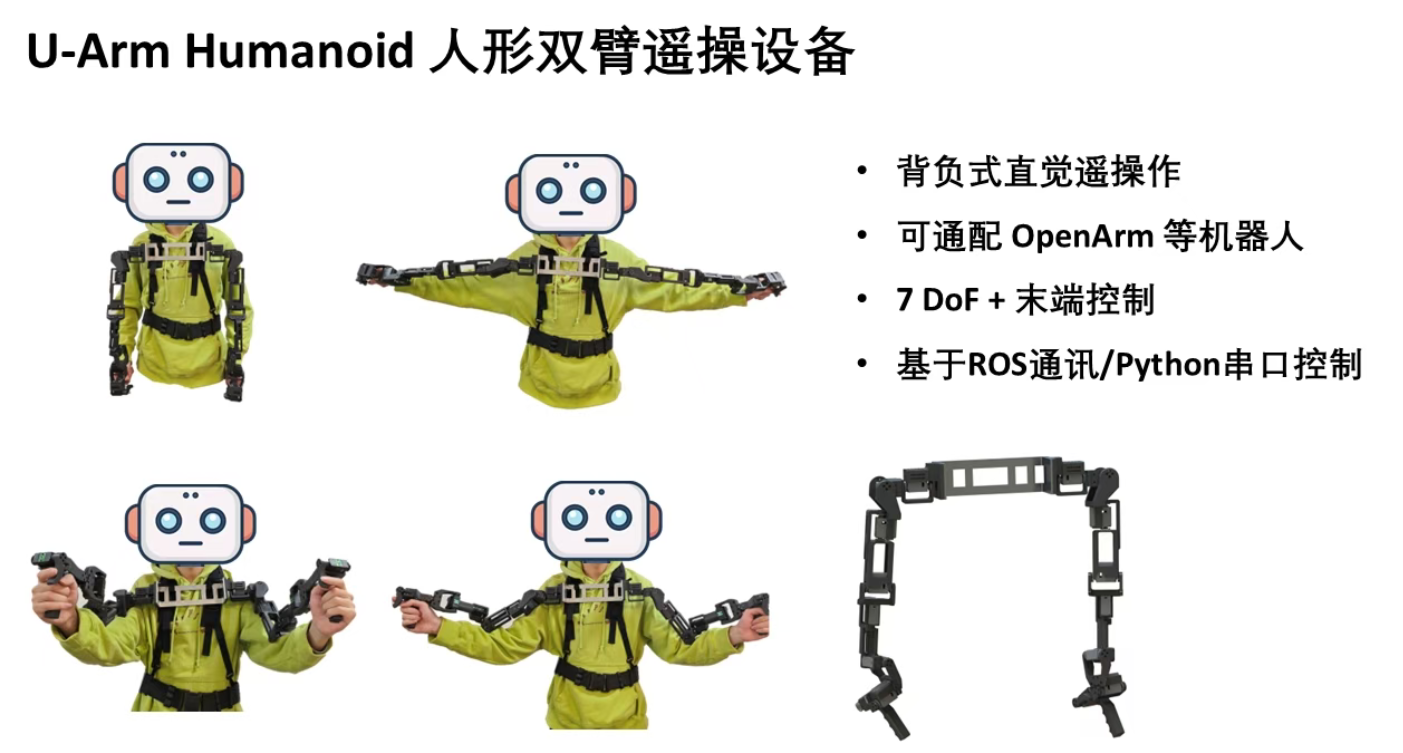
\includegraphics[keepaspectratio]{../../assets/figures/lecture09/ref/figures/fig92-uarm-humanoid.png}}

}

\caption{背负式人形双臂遥操设备}

\end{figure}%

更进一步，让人形机器人实时''影随''人的全身动作，就能在做任务的同时把全身的示教数据录下来------这是
\textbf{HumanPlus} 的做法，下图出自该工作。

\begin{figure}[H]

{\centering \pandocbounded{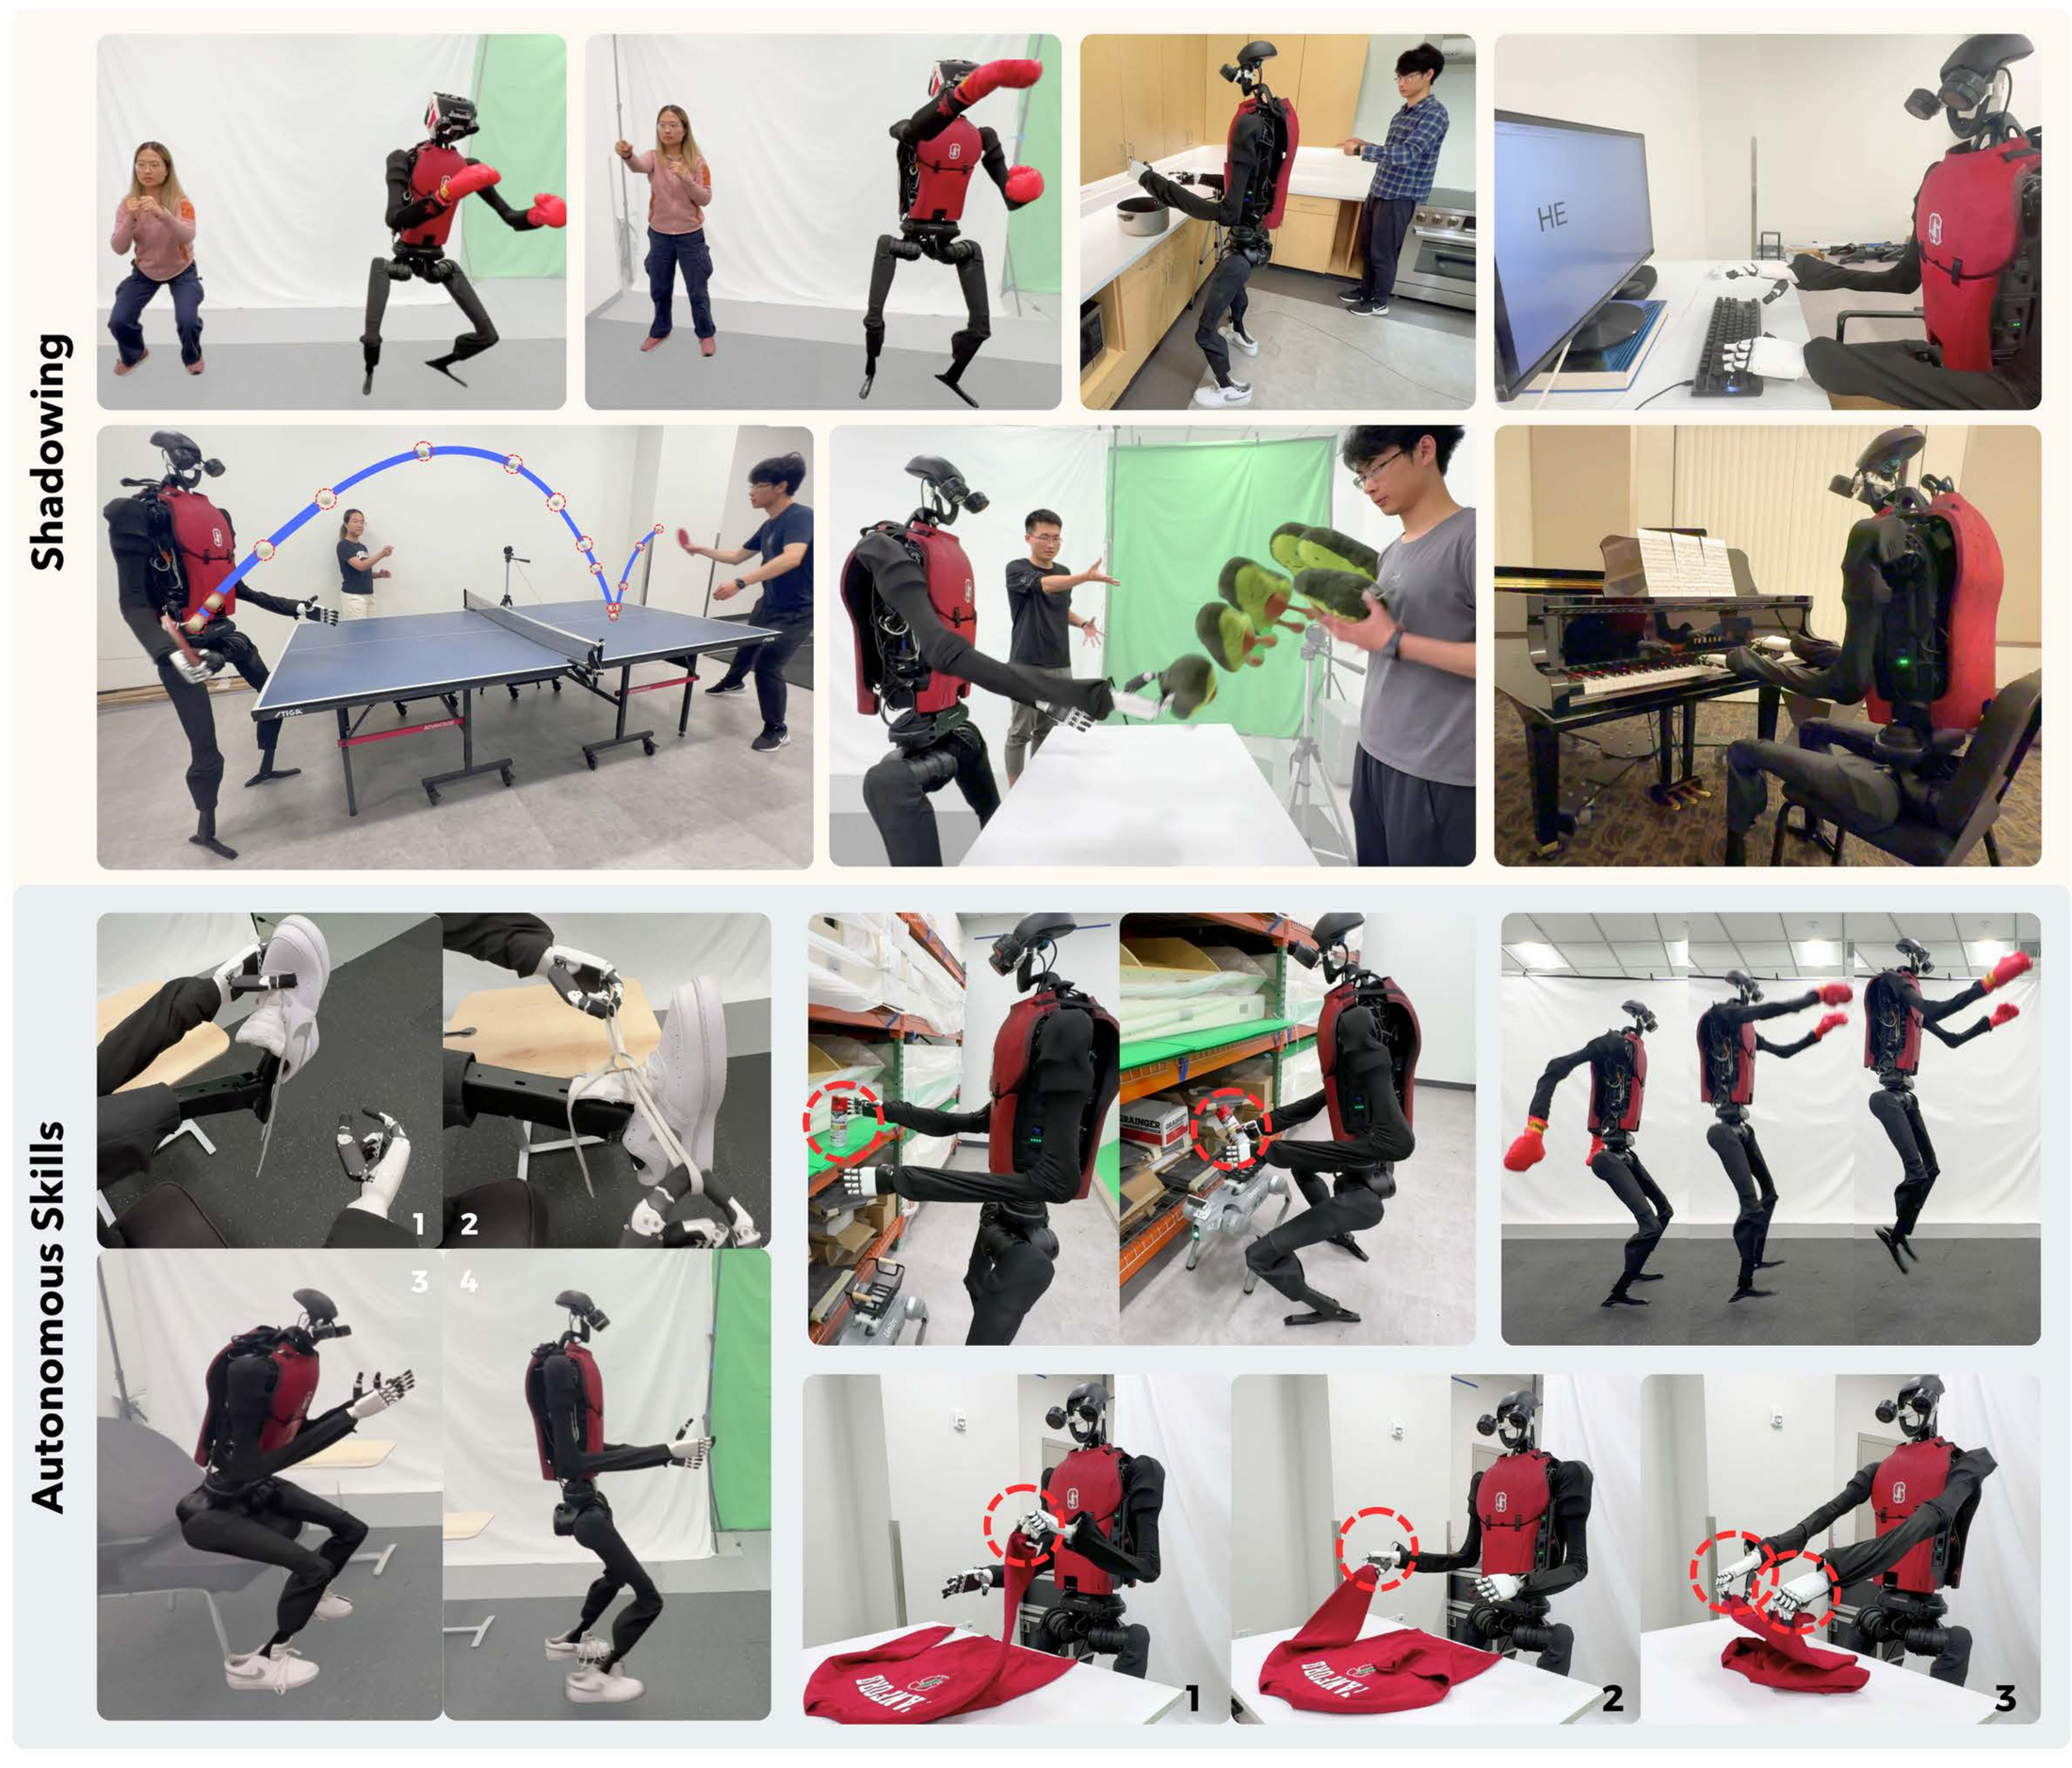
\includegraphics[keepaspectratio]{../../assets/figures/lecture09/ref/figures/fig92-humanplus.png}}

}

\caption{人形机器人实时影随人的动作，边做任务边录全身示教}

\end{figure}%

\subsection{2.4
通用接口遥操作}\label{ux901aux7528ux63a5ux53e3ux9065ux64cdux4f5c}

这一类直接复用现成的、人人都有的输入设备来驱动机器人，门槛极低、易规模化。

\subsubsection{2.4.1 手柄}\label{ux624bux67c4}

最朴素的是用通用游戏手柄驱动机器人采集，下图来自开源项目
\textbf{joycon-robotics}（用任天堂 Joy-Con 手柄遥操）。

\begin{figure}[H]

{\centering \pandocbounded{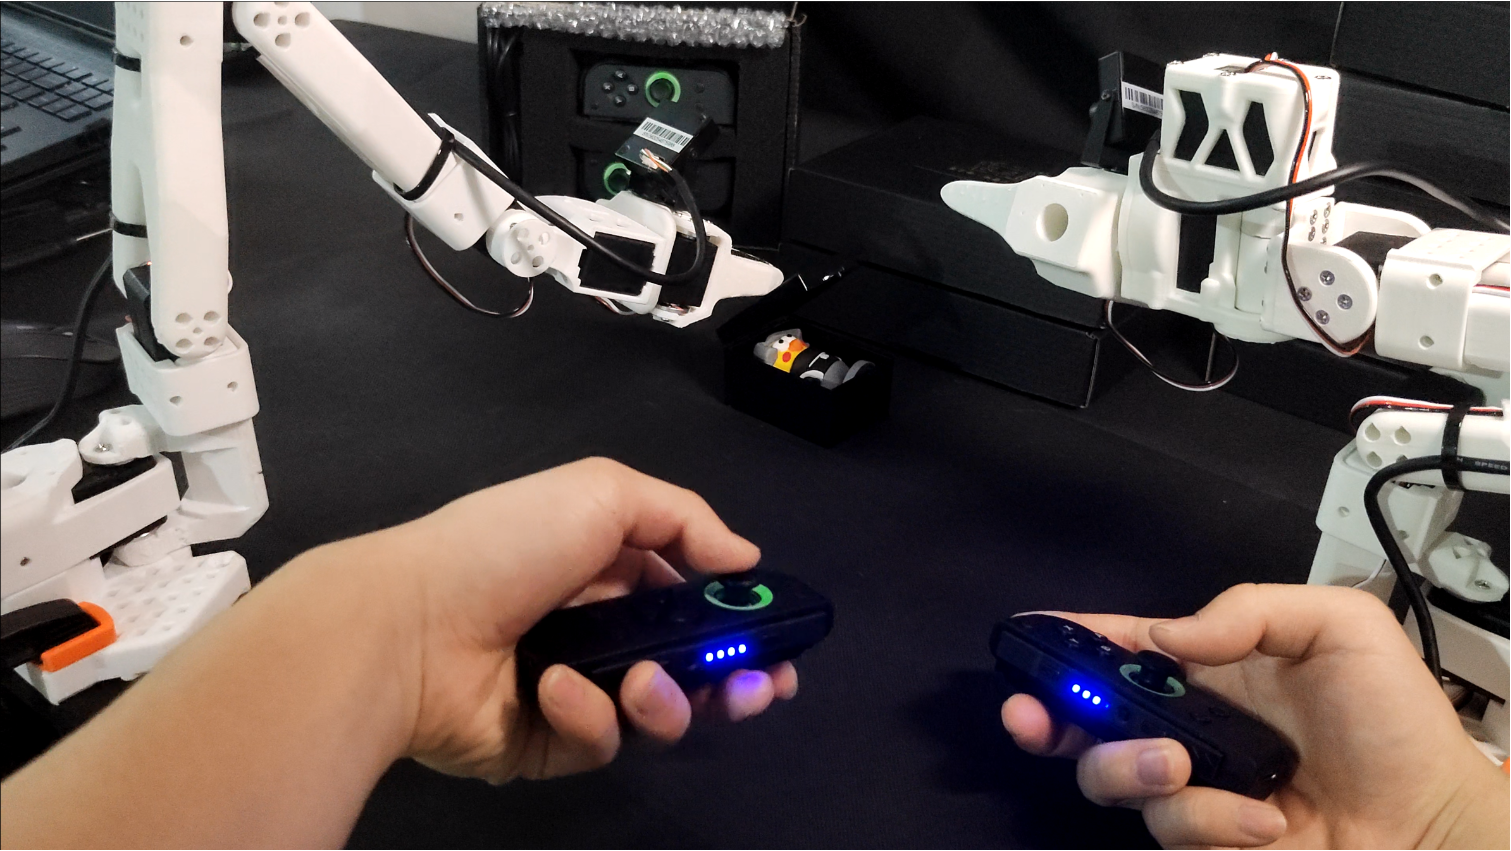
\includegraphics[keepaspectratio]{../../assets/figures/lecture09/ref/figures/fig92-joycon.png}}

}

\caption{用通用手柄驱动主从臂采集}

\end{figure}%

\subsubsection{2.4.2 手机众包}\label{ux624bux673aux4f17ux5305}

\textbf{RoboTurk}
把手机当成六自由度的控制器，再放到云端做众包，远端工人无需培训就能登录网页采集，单个项目就曾众包出上百小时的数据------这说明\textbf{接口越通用，越能把采集规模化}。下图出自该工作。

\begin{figure}[H]

{\centering \pandocbounded{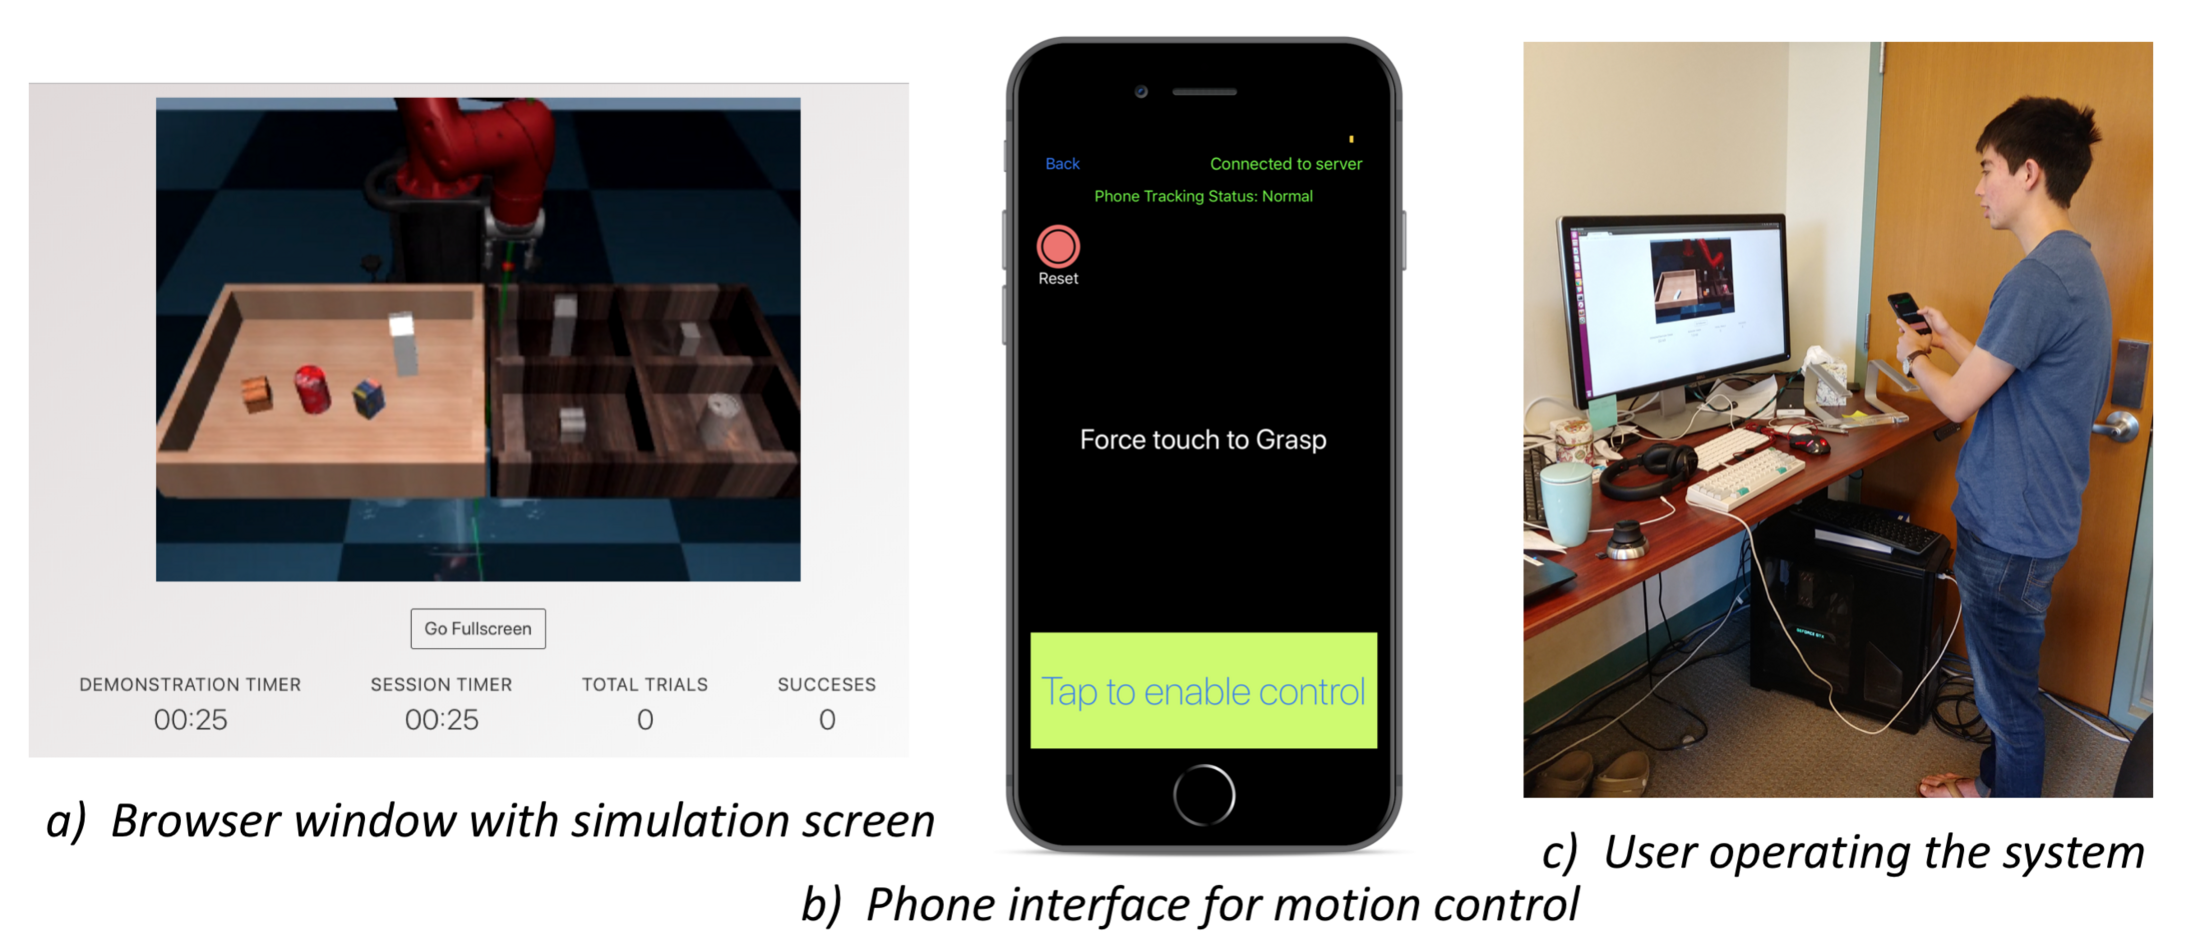
\includegraphics[keepaspectratio]{../../assets/figures/lecture09/ref/figures/fig92-roboturk.png}}

}

\caption{用手机当控制器、在云端众包采集机器人示教}

\end{figure}%

\subsubsection{2.4.3
虚拟现实与增强现实}\label{ux865aux62dfux73b0ux5b9eux4e0eux589eux5f3aux73b0ux5b9e}

戴上头显做沉浸式遥操，可以同时获得立体视觉反馈和手臂、手部的动作映射，操作者像''附身''在机器人上------下图来自
\textbf{Open-TeleVision}。

\begin{figure}[H]

{\centering \pandocbounded{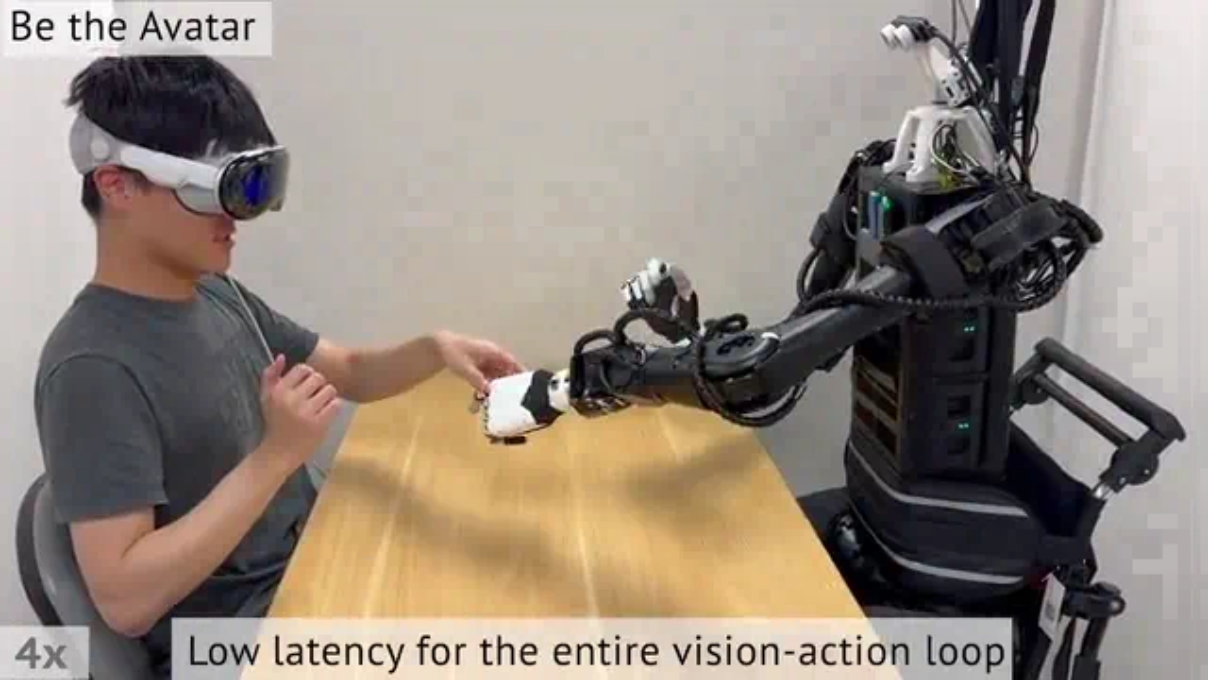
\includegraphics[keepaspectratio]{../../assets/figures/lecture09/ref/figures/fig92-open-television.png}}

}

\caption{沉浸式头显遥操，立体视觉反馈加手臂手部动作映射}

\end{figure}%

基于通用消费级头显的方案（\textbf{OpenTeach}），可以用自然手势驱动机器人，并在很多任务上验证。

\begin{figure}[H]

{\centering \pandocbounded{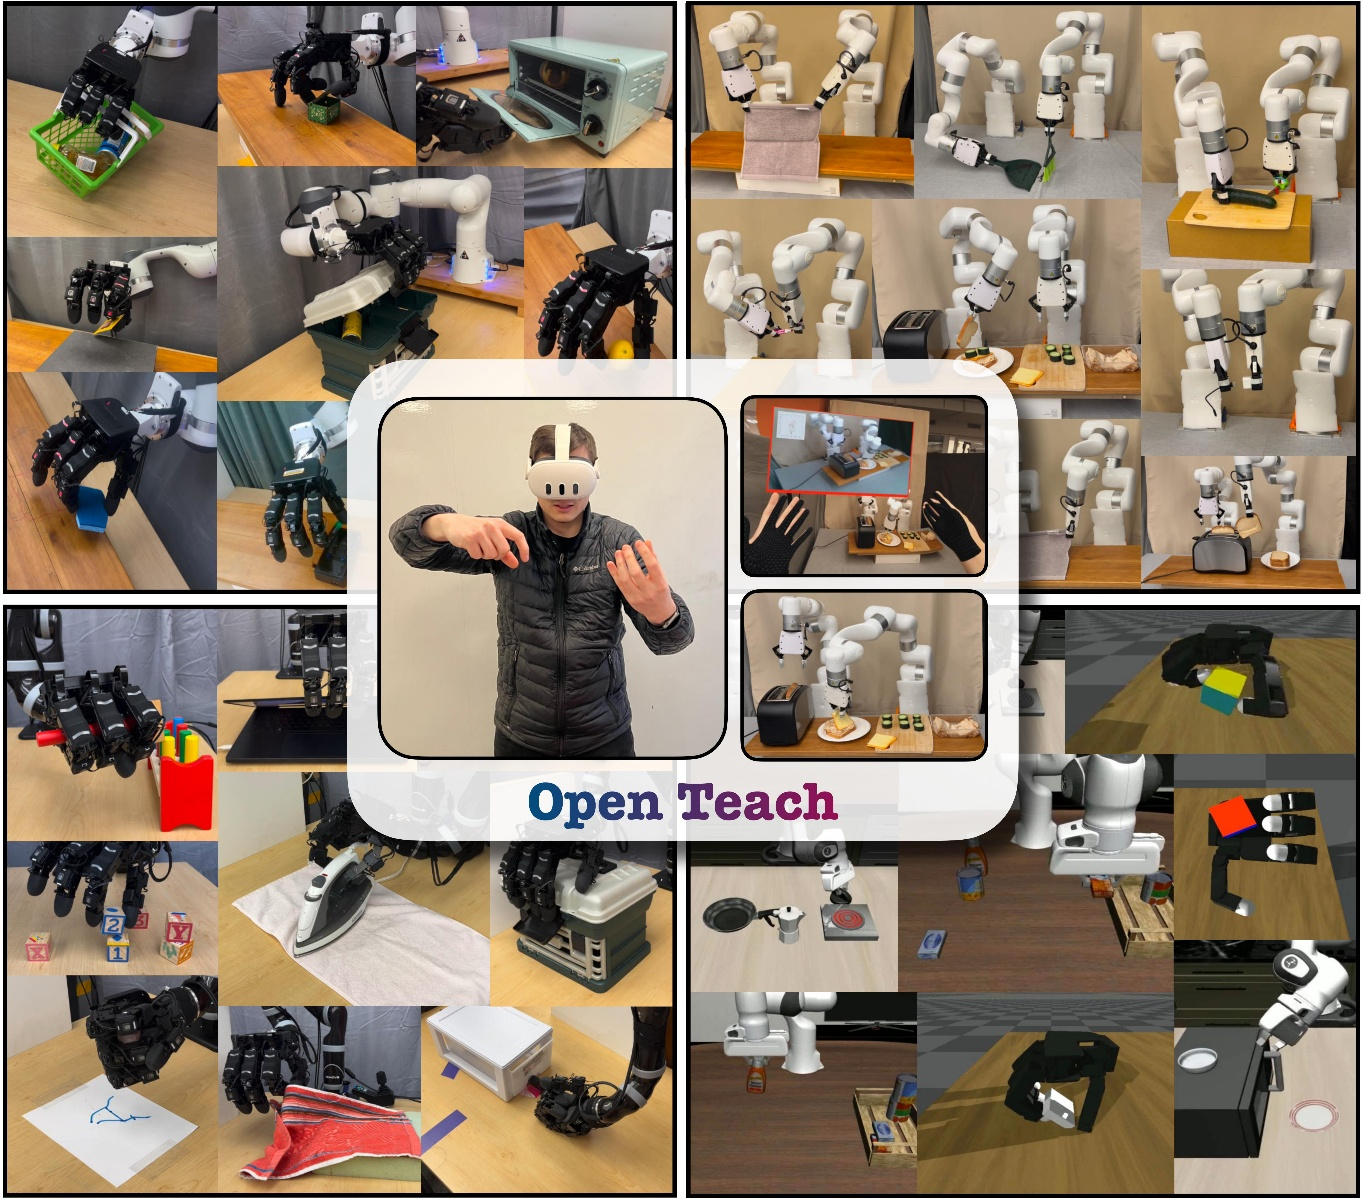
\includegraphics[keepaspectratio]{../../assets/figures/lecture09/ref/figures/fig92-openteach.jpeg}}

}

\caption{基于通用消费级头显的自然手势遥操}

\end{figure}%

借助高端头显，还能做到实时的双臂灵巧遥操，下图来自
\textbf{Bunny-VisionPro}。

\begin{figure}[H]

{\centering \pandocbounded{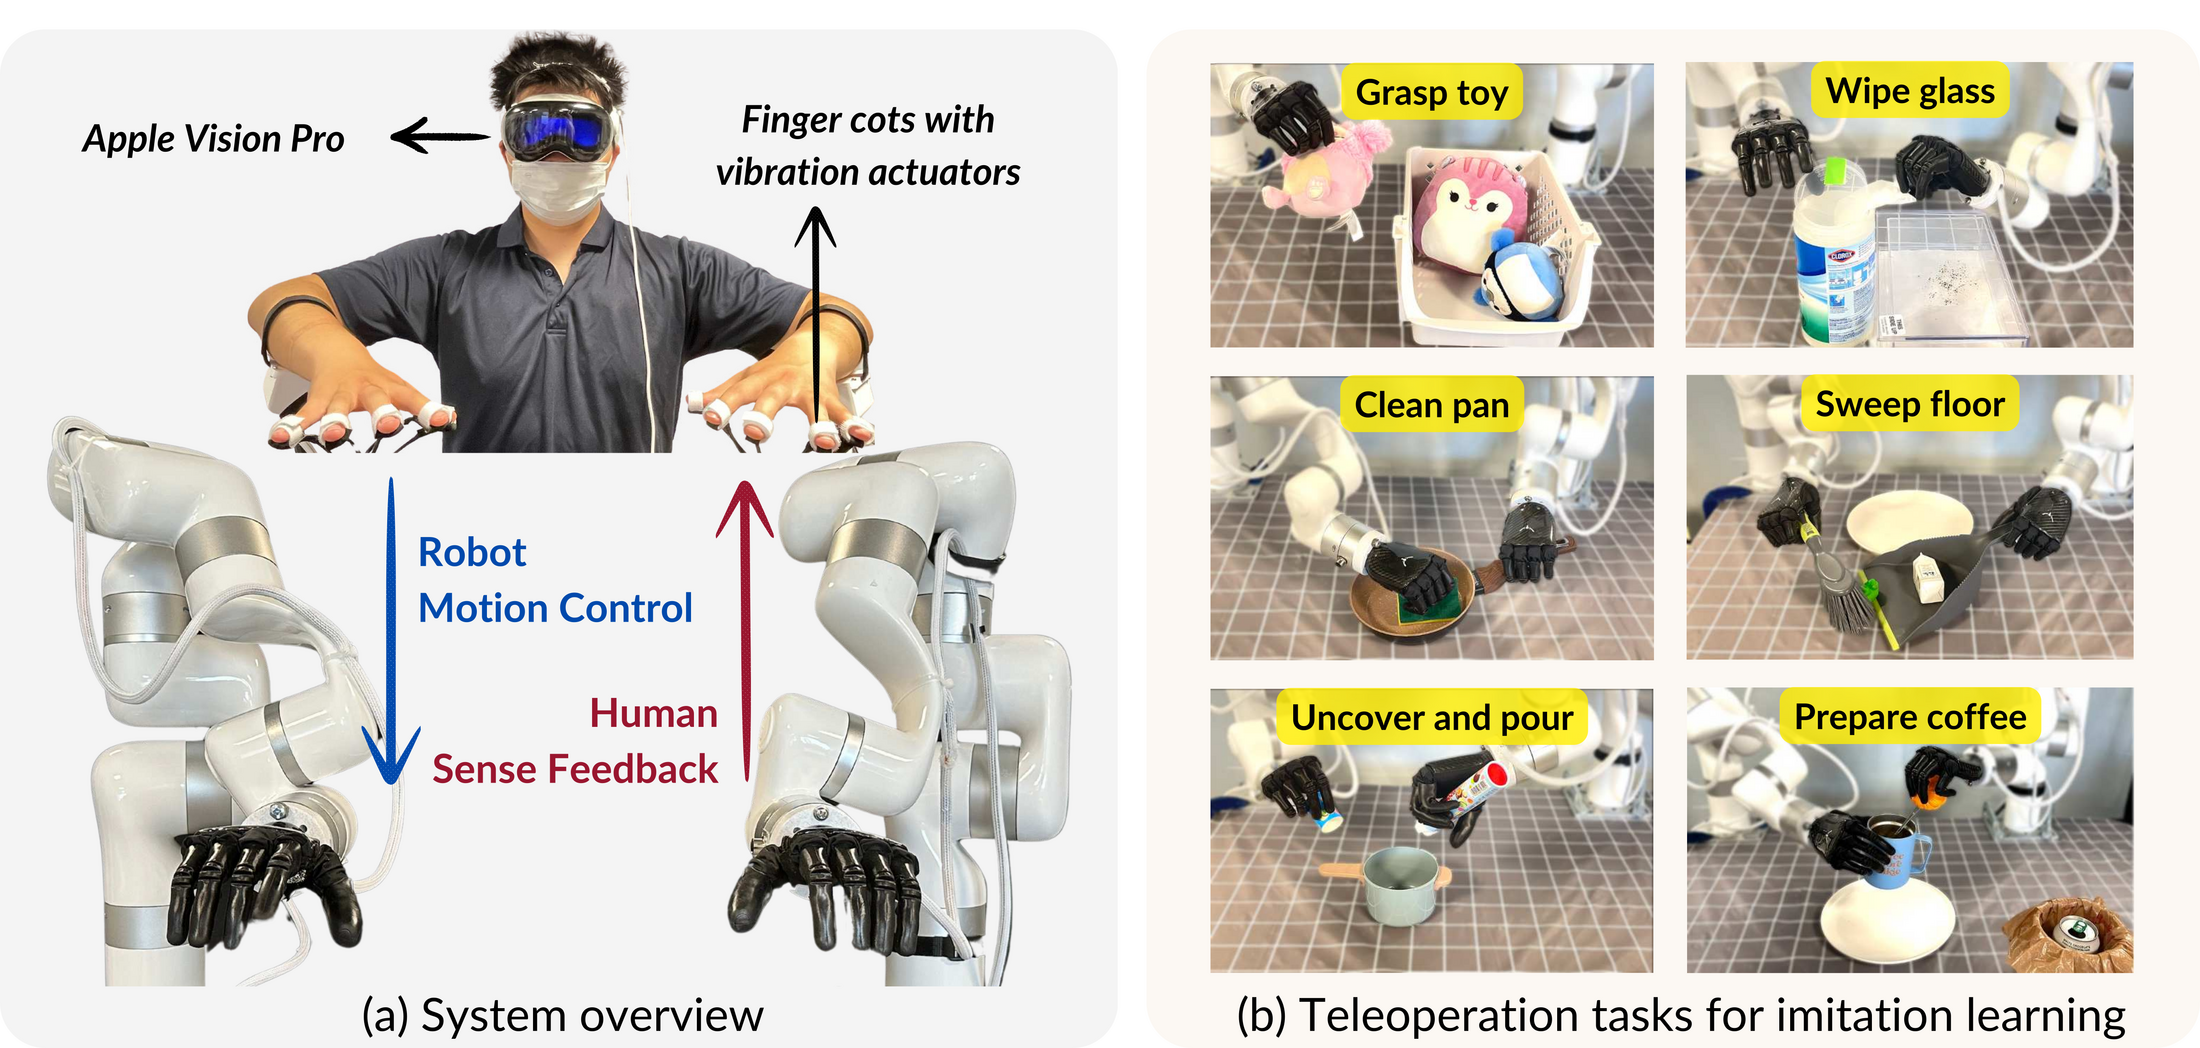
\includegraphics[keepaspectratio]{../../assets/figures/lecture09/ref/figures/fig92-bunny-visionpro.png}}

}

\caption{基于高端头显的实时双臂灵巧遥操}

\end{figure}%

\subsection{2.5
无机器人数据}\label{ux65e0ux673aux5668ux4ebaux6570ux636e}

最轻的一类连人体代理硬件都不必绑定机器人，直接采人做日常操作的数据，再想办法转成机器人能用的监督。它的可规模化程度最高，但''转化''这一步也最重。

\subsubsection{2.5.1
第一视角人类操作数据}\label{ux7b2cux4e00ux89c6ux89d2ux4ebaux7c7bux64cdux4f5cux6570ux636e}

\textbf{In-N-On}
用智能眼镜或头显直接采人做日常操作的第一视角视频，把数据分成''野外随手采''和''贴着目标任务采''两类，先用海量野外数据预训练、再用少量贴任务数据微调，下图出自该工作。

\begin{figure}[H]

{\centering \pandocbounded{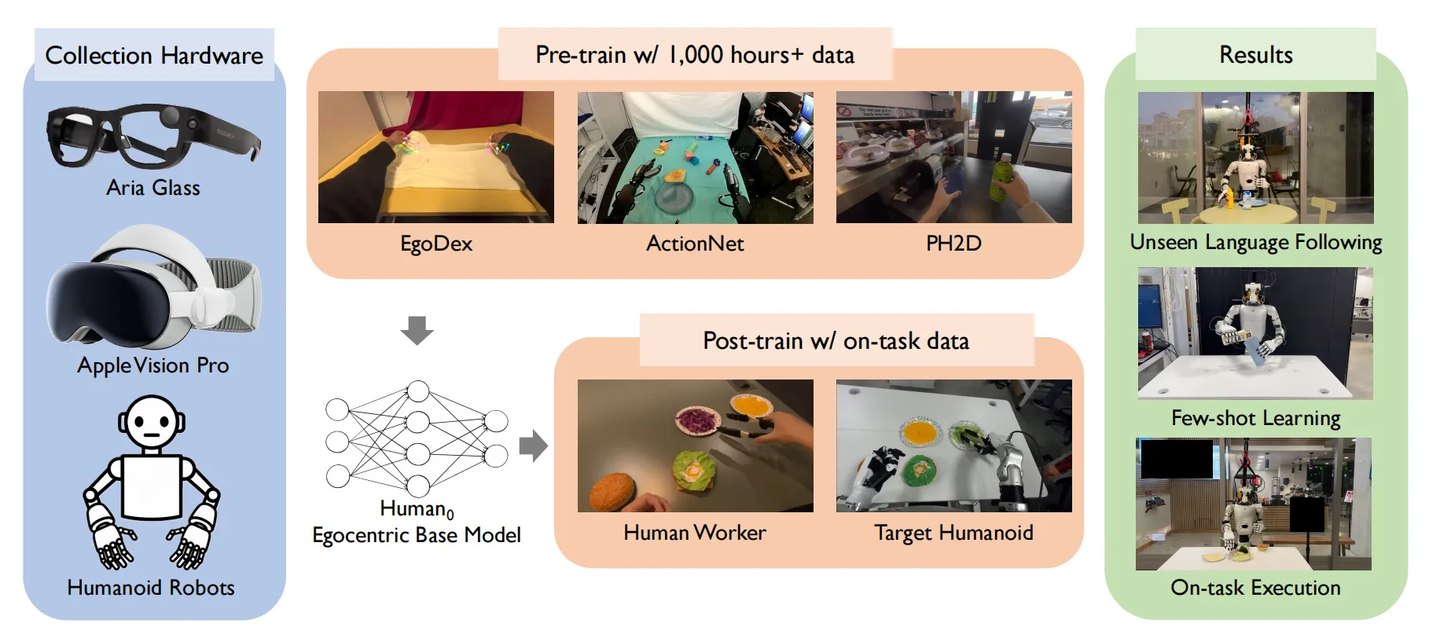
\includegraphics[keepaspectratio]{../../assets/figures/lecture09/ref/figures/fig92-innon.png}}

}

\caption{用第一视角采集人类操作数据，分野外与贴任务两类使用}

\end{figure}%

\subsubsection{2.5.2
世界模型生成数据}\label{ux4e16ux754cux6a21ux578bux751fux6210ux6570ux636e}

更激进的一步（\textbf{Ctrl-World}）是让世界模型在策略的闭环里
rollout，直接合成轨迹来扩充数据，用生成的数据进一步提升策略表现，下图出自该工作。

\begin{figure}[H]

{\centering \pandocbounded{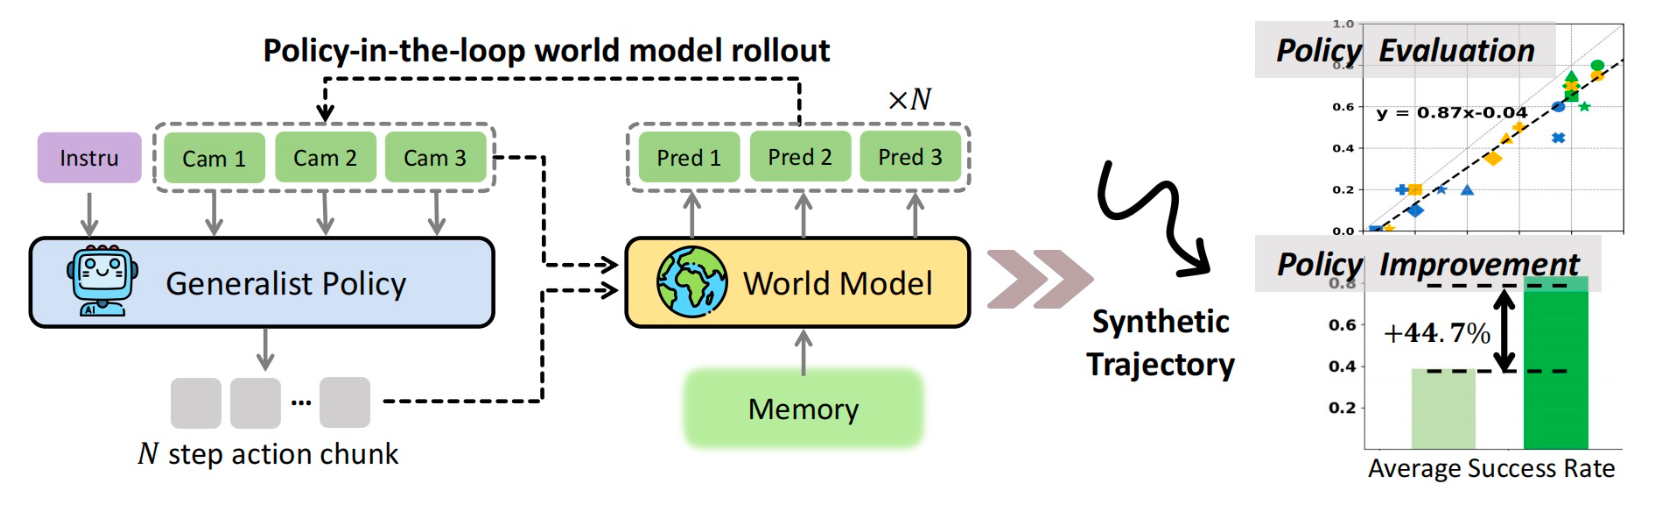
\includegraphics[keepaspectratio]{../../assets/figures/lecture09/ref/figures/fig92-ctrlworld.png}}

}

\caption{让世界模型在策略闭环中 rollout，合成轨迹用于扩充数据}

\end{figure}%

\subsection{2.6
方法对比与落到本课}\label{ux65b9ux6cd5ux5bf9ux6bd4ux4e0eux843dux5230ux672cux8bfe}

把四大类里的代表方法放在一张表里横向看，就能按手上的预算、场地、是否需要力触觉来选型：

\begin{center}
\begin{tabular}{@{}>{\raggedright\arraybackslash}p{\dimexpr 0.2676\linewidth - 2\tabcolsep\relax} >{\raggedright\arraybackslash}p{\dimexpr 0.1494\linewidth - 2\tabcolsep\relax} >{\raggedright\arraybackslash}p{\dimexpr 0.2085\linewidth - 2\tabcolsep\relax} >{\raggedright\arraybackslash}p{\dimexpr 0.1642\linewidth - 2\tabcolsep\relax} >{\raggedright\arraybackslash}p{\dimexpr 0.1199\linewidth - 2\tabcolsep\relax} >{\raggedright\arraybackslash}p{\dimexpr 0.0903\linewidth - 2\tabcolsep\relax}@{}}
\toprule\noalign{}
方法 & 所属大类 & 机器人在回路 & 力 / 触觉 & 成本 & 便携 \\
\midrule\noalign{}
原机示教 & 真机 & 是 & 有 & 中 & 低 \\
主从臂（同构） & 真机 & 是 & 多无 & 低到中 & 低 \\
主从臂（异构） & 真机 & 是 & 无 & 低 & 低 \\
移动整机遥操 & 真机 & 是 & 无 & 中 & 中 \\
手持末端代理 & 人类代理 & 否 & 多无 & 低 & 高 \\
增强现实反馈采集 & 人类代理 & 否 & 视觉提示 & 低 & 高 \\
穿戴代理 & 人类代理 & 否 & 有 & 中 & 中 \\
手柄 & 通用接口 & 是 & 无 & 极低 & 高 \\
手机众包 & 通用接口 & 是 & 无 & 极低 & 高 \\
头显遥操 & 通用接口 & 是 & 部分 & 中 & 中 \\
第一视角 & 无机器人 & 否 & 无 & 低 & 极高 \\
世界模型生成 & 无机器人 & 否 & 无 & 算力 & 高 \\
\bottomrule\noalign{}
\end{tabular}
\end{center}

落到本课：实物实验用 SO-101
主从臂（真机、同构），它是这张地图里成本最低的入口；没有真机时，就用
SO-101
仿真器配手柄或键盘（对应通用接口那一类），落成同一种容器格式的数据。仿真里还有一条\textbf{完全不靠人遥操}的路：让一个视觉强化学习策略在仿真里从零学会任务、自动跑出成功轨迹充当训练数据------本课后面用来微调
VLA 的那批 SO-101 仿真数据，正是这么来的，第16讲会把这套''视觉 RL
生成数据''的做法从头讲透。但在动手采之前，得先认清一件事：不管用哪种方法，采到的数据最终都要以\textbf{同一种标准格式}落盘、被训练代码直接读。下一节就把承载这一切的
\textbf{LeRobot 框架与数据集格式}讲清楚，再回头动手采。

\section{3 LeRobot
框架与数据集}\label{lerobot-ux6846ux67b6ux4e0eux6570ux636eux96c6}

上一节铺完了各种采集方法。但不管用哪种方法，采到的数据最终都要以\textbf{同一种标准格式}落盘、被训练代码直接读------否则每换一种机器人、每换一种算法都要重写一遍工具链。这套把数采、数据、训练串起来的框架，就是
HuggingFace 推出的 \textbf{LeRobot}。这一节先认清它，下一节再动手采。

\subsection{3.1 LeRobot
是什么：一条端到端的闭环}\label{lerobot-ux662fux4ec0ux4e48ux4e00ux6761ux7aefux5230ux7aefux7684ux95edux73af}

LeRobot 是 HuggingFace 推出的\textbf{端到端具身智能开源框架}（Apache-2.0
许可、PyTorch
实现），目标是降低机器人学习的门槛。它把从硬件接口、数据采集、数据格式、策略训练到推理部署的整条栈，串成一个\textbf{闭环}：

\begin{figure}[H]

{\centering 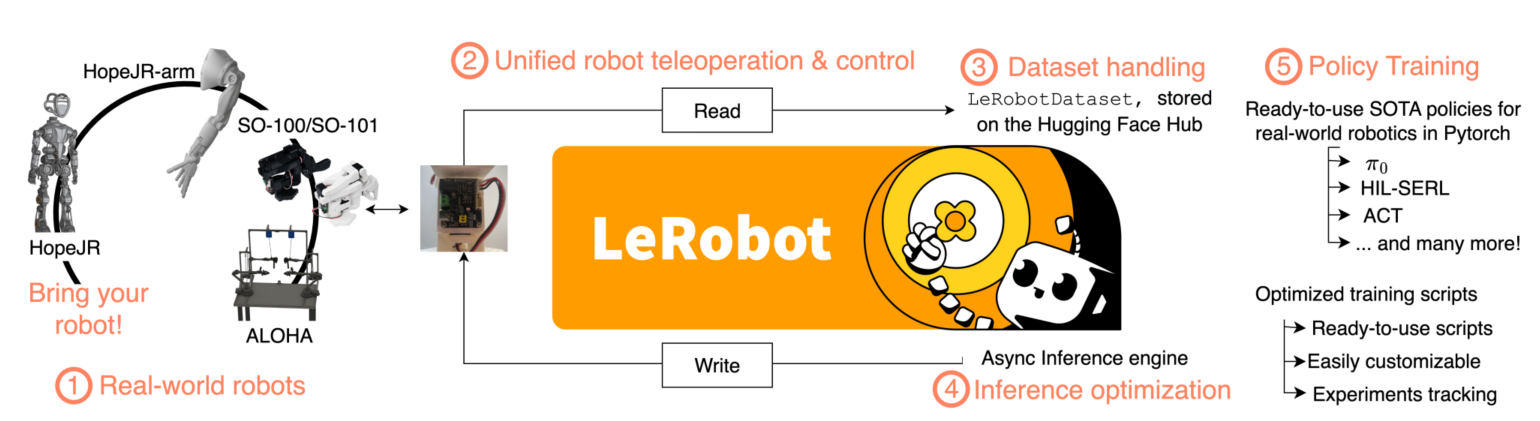
\includegraphics[width=0.98\linewidth,height=\textheight,keepaspectratio]{../../assets/figures/lecture09/ref/figures/fig93-lerobot-overview.png}

}

\caption{LeRobot 串起的闭环，真实机器人到遥操作采集到数据集（托管在
HuggingFace Hub）到策略训练（\(\pi_0\) / HIL-SERL / ACT）再到推理部署}

\end{figure}%

顺着图上的五块走一圈：\textbf{Real-world
robots}（带上你自己的机器人，SO-100/SO-101、ALOHA、HopeJR\ldots\ldots）→
\textbf{Unified teleoperation \& control}（用统一接口遥操作驱动它）→
\textbf{Dataset handling}（把过程录成 LeRobotDataset 并存到 HuggingFace
Hub）→ \textbf{Policy training}（用 Hub 上现成的 SOTA 策略训练 / 微调）→
\textbf{Inference
optimization}（经异步推理引擎部署回机器人）。本讲走的就是中间「采集 →
数据集」这一段，下一讲接「策略训练」。

把这个闭环落到代码里，LeRobot
是一套\textbf{自上而下的分层架构}------每一层只管自己的事，上层调用下层的抽象，所以换机器人只动底层、换算法只动策略层：

\begin{figure}[H]

{\centering 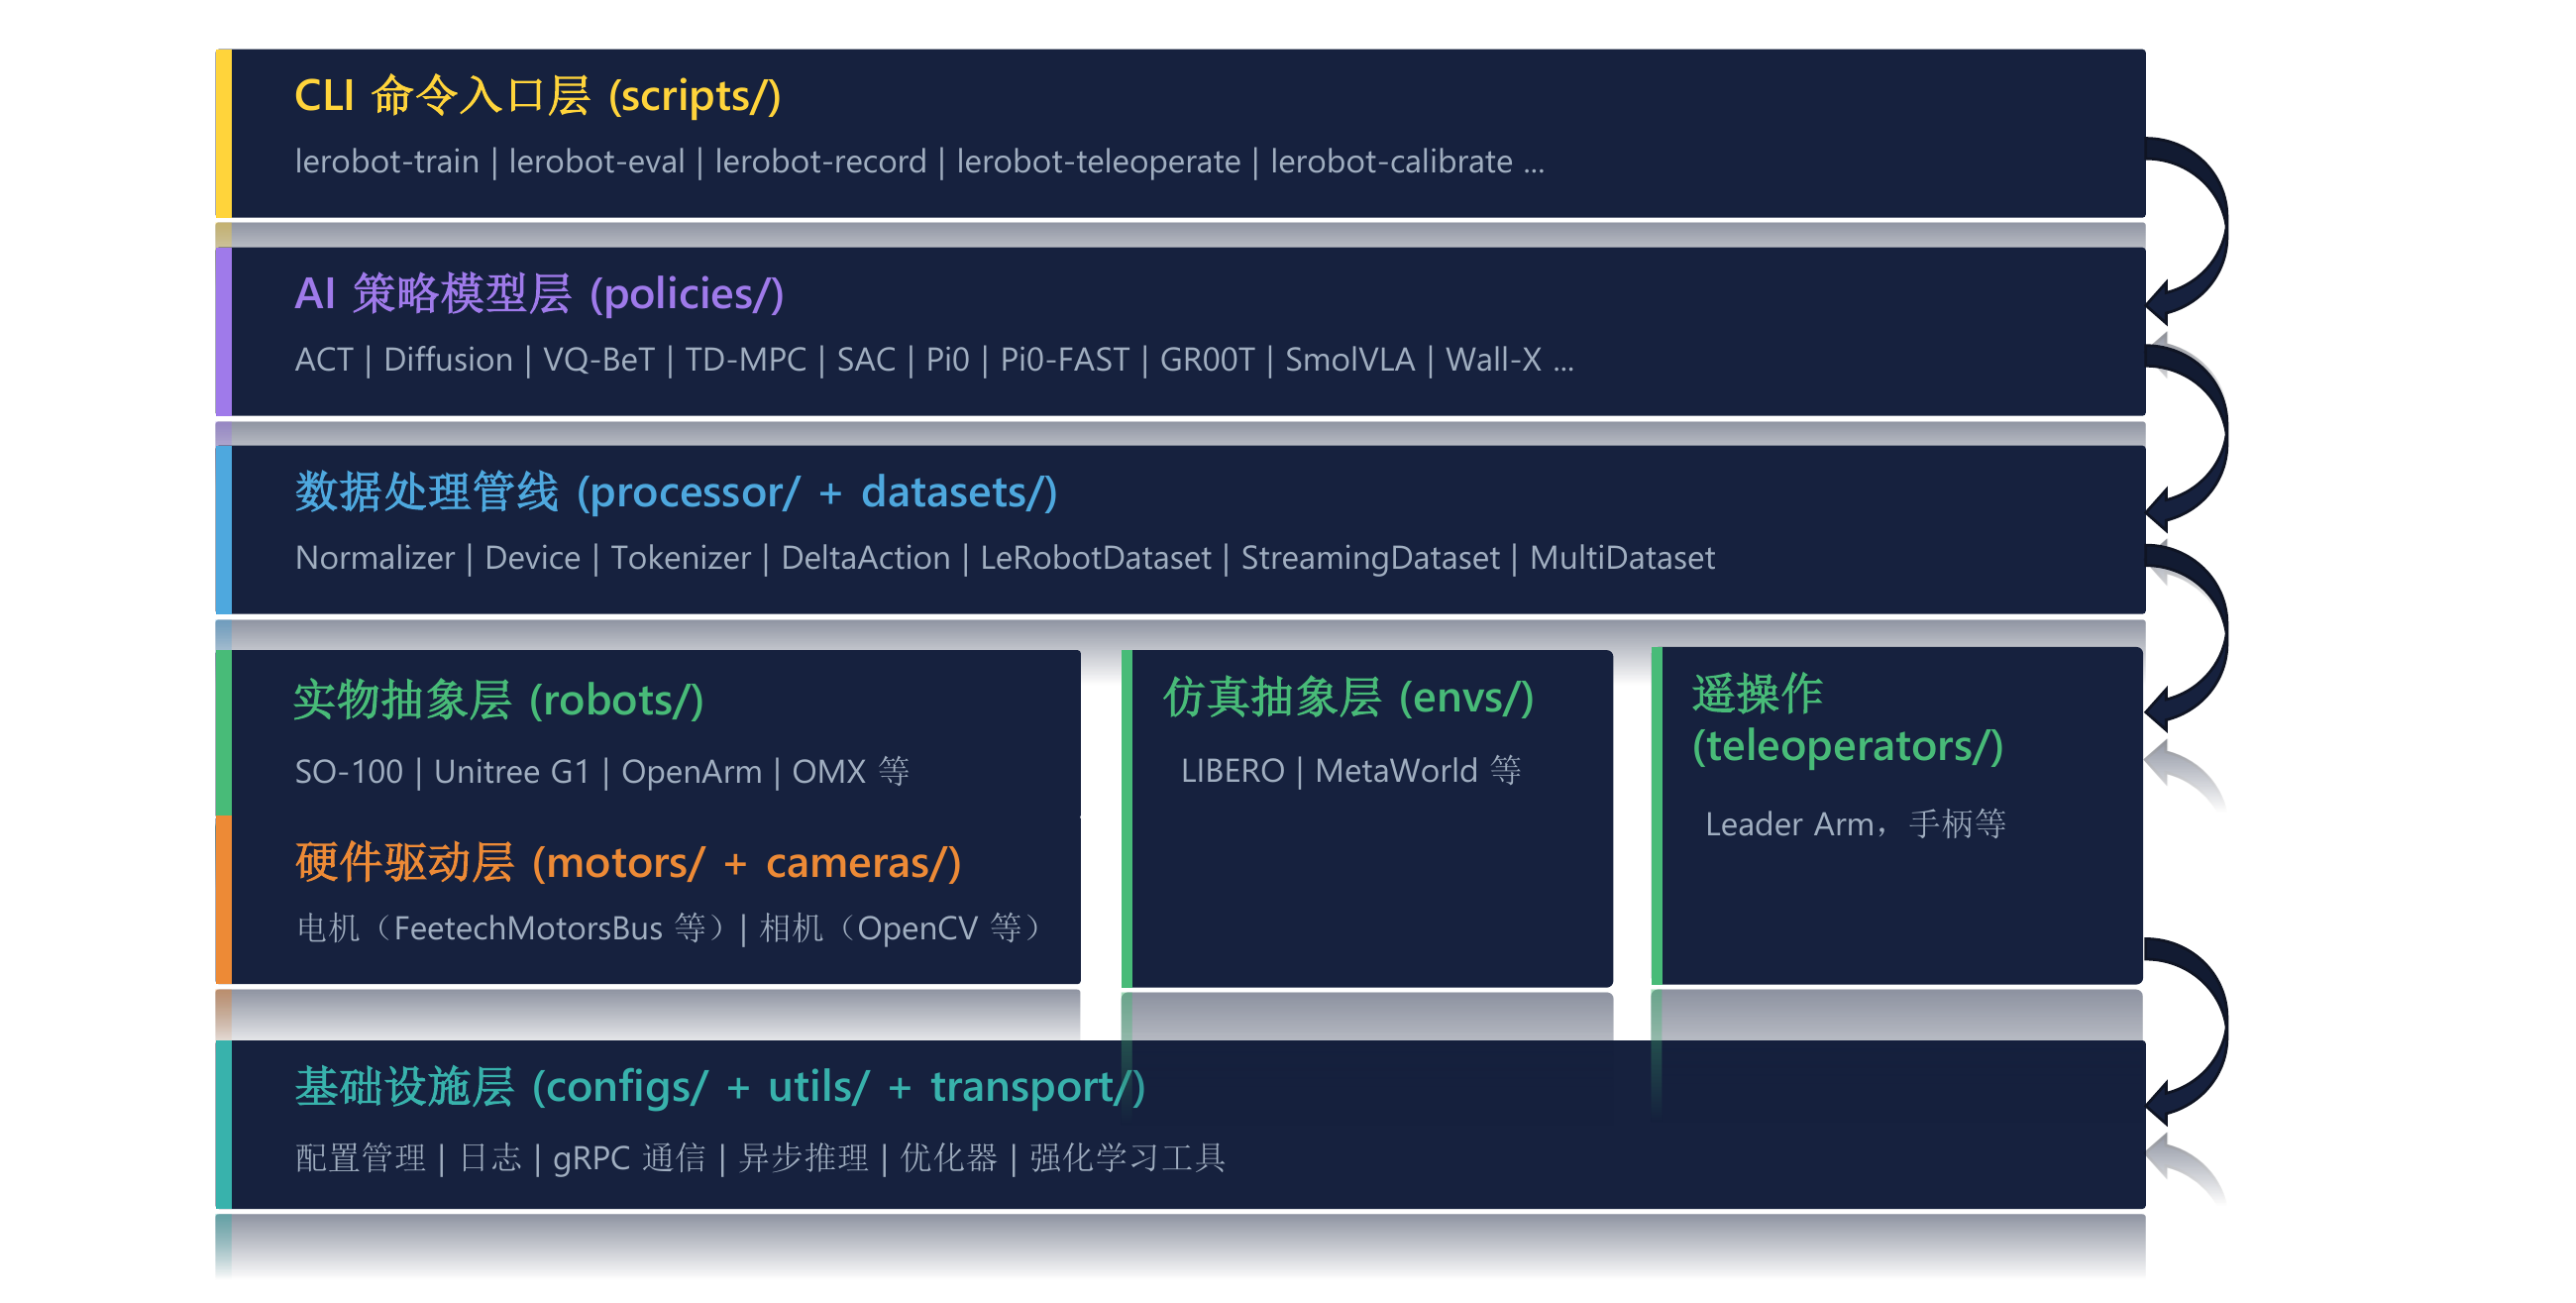
\includegraphics[width=0.98\linewidth,height=\textheight,keepaspectratio]{../../assets/figures/lecture09/ref/figures/fig93-lerobot-arch.png}

}

\caption{LeRobot 自上而下的分层代码架构总览：CLI 命令入口层 / AI
策略模型层 / 数据处理管线 / 实物与仿真抽象层 / 遥操作器 / 基础设施层}

\end{figure}%

从上往下看：\textbf{CLI 命令入口层（scripts/）} 提供
\texttt{lerobot-record}/\texttt{lerobot-train} 等命令，\textbf{AI
策略模型层（policies/）} 放 ACT / Diffusion / \(\pi_0\) / SmolVLA
等算法，\textbf{数据处理管线（processor/ + datasets/）}
管统一数据格式，\textbf{实物抽象层（robots/）}
与\textbf{仿真抽象层（envs/）} 分别接真机（SO-100、Unitree
G1\ldots\ldots）和仿真（LIBERO、MetaWorld\ldots\ldots），\textbf{遥操作器（teleoperators/）}
提供主臂 / 手柄等输入，最底下是\textbf{基础设施层（configs/ + utils/ +
transport/）}。换机器人只动 \texttt{robots/}、换算法只动
\texttt{policies/}，彼此不牵连。

\subsection{3.2
数据采集落在哪一层}\label{ux6570ux636eux91c7ux96c6ux843dux5728ux54eaux4e00ux5c42}

在这套分层里，与「采数据」直接相关的只有两层------把它们在同一张图上用红框高亮出来：

\begin{figure}[H]

{\centering 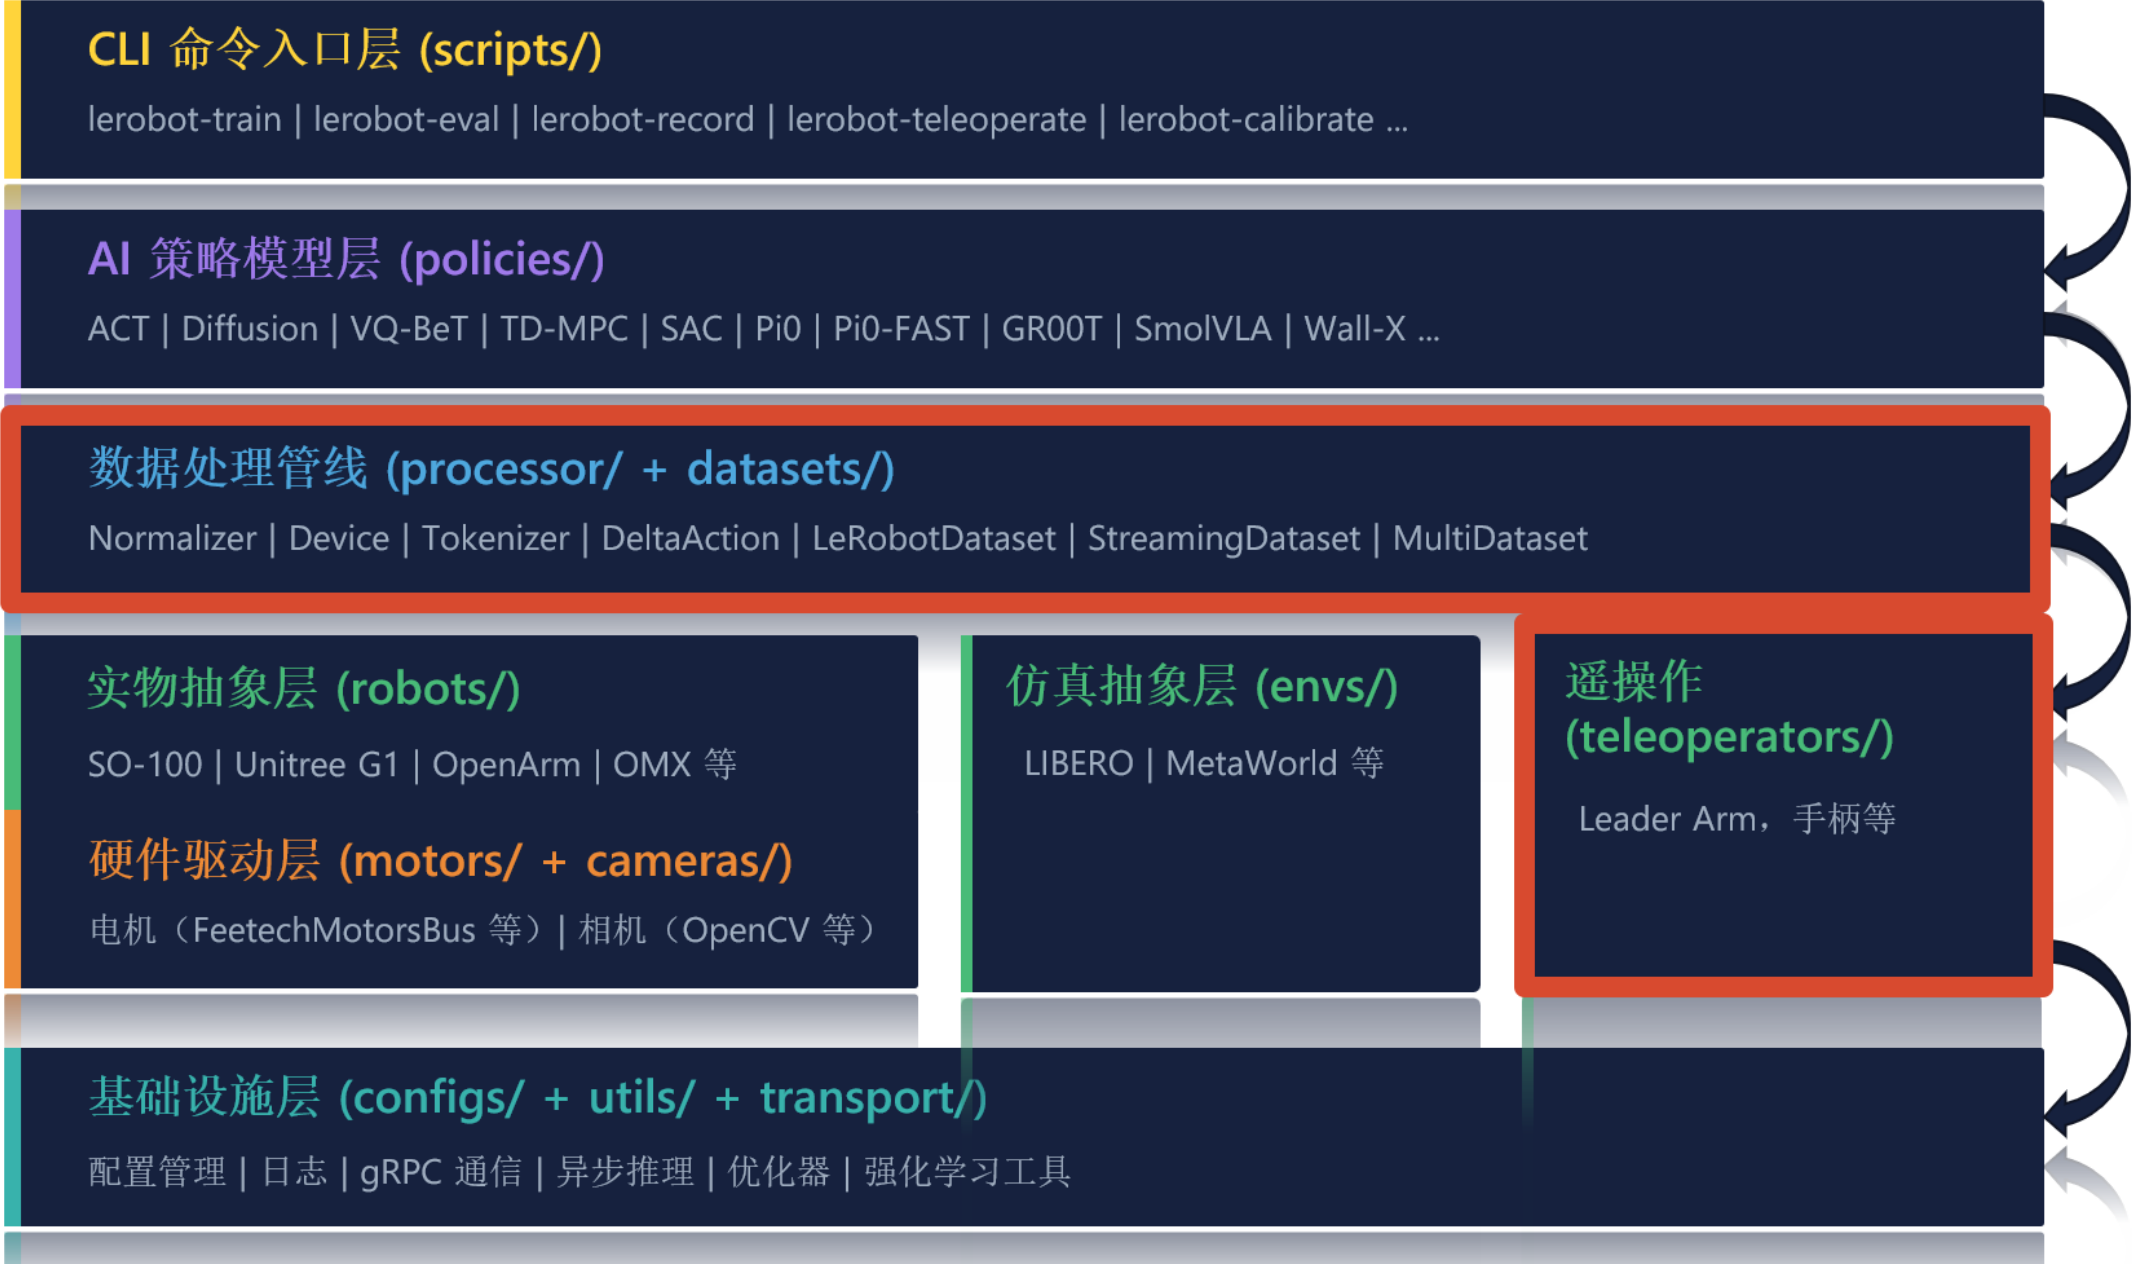
\includegraphics[width=0.98\linewidth,height=\textheight,keepaspectratio]{../../assets/figures/lecture09/ref/figures/fig93-lerobot-arch-highlight.png}

}

\caption{数据采集在 LeRobot
框架中的位置：红框标出的数据处理管线（datasets/）负责落盘、遥操作器（teleoperators/）负责驱动}

\end{figure}%

红框圈出的两块就是本讲焦点：\textbf{数据处理层（datasets/）}
负责把采到的东西落成统一格式，\textbf{遥操作器（teleoperators/）}
负责驱动机器人产生动作。我们用 \textbf{CLI 入口层}的
\texttt{lerobot-record} 采数据（第 4
节），它向下调用\textbf{实物抽象层}的
SO-101（机器人本体）和\textbf{遥操作器}的主臂；采出来的，就是\textbf{数据处理层}里的一份
LeRobotDataset。下面先把这个格式认全。

\subsection{3.3
LeRobotDataset：采集到训练的统一格式}\label{lerobotdatasetux91c7ux96c6ux5230ux8badux7ec3ux7684ux7edfux4e00ux683cux5f0f}

LeRobotDataset 是 HuggingFace
为机器人学习设计的\textbf{统一数据格式}，专门存储和共享多模态时序数据（传感器信号
+ 多相机视频）。它有三条核心设计：\textbf{存储与 API
解耦}（底层是少量大文件、上层提供直观的 episode 级访问）、\textbf{Hub
原生}（直接在 HuggingFace Hub
上托管、搜索、可视化）、\textbf{流式支持}（无需下载即可消费数据）。

\begin{quote}
备注（版本口径）：本节及后文的目录结构、\texttt{meta/}
字段、类名与源码文件位置，都基于 \textbf{LeRobot \textgreater=
0.4.0、LeRobotDataset v3.0，核验日期 2026-07-21}。LeRobot
是一个迭代很快的库，目录布局、CLI
参数名和源码文件名都可能随版本变动。照着跑之前先确认自己装的版本；对不上时以官方文档与当前源码为准。
\end{quote}

先记住一个最小单位------\textbf{episode（回合）}：就是机器人把某个任务从头到尾做一遍的完整记录，从初始状态开始、到任务结束为止，期间每一帧的图像、关节状态、动作都按时间顺序记下来。一个数据集，就是许许多多
episode 的集合（行为克隆里常见 50\textasciitilde100 个起步）。

落到磁盘上，LeRobotDataset
把一份采集拆成\textbf{三大支柱}分开存：\textbf{低维数据进 Parquet
表格、相机画面进 MP4 视频、说明书进 meta}。

\dirtree{%
.1 \texttt{<dataset>/} {\color{TreeNoteColor}（一份采集，HF 缓存目录下）}.
.2 \texttt{data/} {\color{TreeNoteColor}（表格：状态 / 动作 / 时间戳 / 索引，列式 parquet）}.
.3 \texttt{chunk-000/}.
.4 \texttt{file-000.parquet} {\color{TreeNoteColor}（多个 episode 的行合并到同一文件）}.
.2 \texttt{videos/} {\color{TreeNoteColor}（视频：每路相机一个子目录）}.
.3 \texttt{observation.images.front/} {\color{TreeNoteColor}（前视相机）}.
.4 \texttt{chunk-000/file-000.mp4} {\color{TreeNoteColor}（多个 episode 的帧合并到同一视频）}.
.3 \texttt{observation.images.side/} {\color{TreeNoteColor}（侧视相机）}.
.2 \texttt{meta/} {\color{TreeNoteColor}（数据集说明书）}.
.3 \texttt{info.json} {\color{TreeNoteColor}（schema：字段、维度、帧率、路径模板）}.
.3 \texttt{stats.json} {\color{TreeNoteColor}（全局统计 mean/std/min/max，训练归一化）}.
.3 \texttt{tasks.parquet} {\color{TreeNoteColor}（任务描述到整数 ID 的映射）}.
.3 \texttt{episodes/} {\color{TreeNoteColor}（每 episode 的长度、任务、文件偏移量）}.
}

三大支柱各管一摊：

\begin{center}
\begin{tabular}{@{}>{\raggedright\arraybackslash}p{\dimexpr 0.1429\linewidth - 2\tabcolsep\relax} >{\raggedright\arraybackslash}p{\dimexpr 0.2612\linewidth - 2\tabcolsep\relax} >{\raggedright\arraybackslash}p{\dimexpr 0.5959\linewidth - 2\tabcolsep\relax}@{}}
\toprule\noalign{}
支柱 & 存什么 & 怎么存 \\
\midrule\noalign{}
表格 \texttt{data/} & 低维、高频信号：关节状态、动作、时间戳、各种索引 & 列式 Apache Parquet，多 episode 行级拼接到大文件，支持内存映射与流式读取 \\
视频 \texttt{videos/} & 相机画面这类高维数据 & 每路相机编码成 MP4（默认 AV1 高压缩，可选 H.264/H.265），多 episode 帧拼接 \\
元数据 \texttt{meta/} & 整份数据集的结构与口径 & \texttt{info.json}（schema）+ \texttt{stats.json}（归一化统计）+ \texttt{tasks.parquet}（任务表）+ \texttt{episodes/}（每条边界） \\
\bottomrule\noalign{}
\end{tabular}
\end{center}

\begin{quote}
备注：新版（v3.0）把许多 episode 的行\textbf{合并}进同一个
\texttt{file-000.parquet}、帧合并进同一个 \texttt{file-000.mp4}，某条
episode 的边界靠 \texttt{meta/episodes/}
里记录的偏移量定位。这样做是为了减少文件数、降低文件系统压力、让 Hub
大文件下载更高效。\textbf{这套结构与采集方式无关}------不管是 SO-101
真机遥操还是仿真器键盘采，最后都长成这个样子。
\end{quote}

这种''把许多 episode 合并进大文件''的组织方式，正是 v3.0 相比老版 v2.0
最关键的改动。两版差别一表看清：

\begin{center}
\begin{tabular}{@{}>{\raggedright\arraybackslash}p{\dimexpr 0.1823\linewidth - 2\tabcolsep\relax} >{\raggedright\arraybackslash}p{\dimexpr 0.3438\linewidth - 2\tabcolsep\relax} >{\raggedright\arraybackslash}p{\dimexpr 0.4740\linewidth - 2\tabcolsep\relax}@{}}
\toprule\noalign{}
特性 & v2.0 & v3.0（本课所用） \\
\midrule\noalign{}
文件组织 & 每个 episode 一个文件 & 多个 episode 合并到大文件 \\
文件命名 & \texttt{episode-0000.parquet} & \texttt{file-000.parquet} \\
episode 边界 & 直接靠文件名区分 & 靠 \texttt{meta/episodes/} 里的偏移量定位 \\
流式读取 & 不支持 & 支持 \texttt{StreamingLeRobotDataset} \\
文件系统压力 & 高（大量小文件） & 低（少量大文件） \\
Hub 流式下载 & 不支持 & 原生支持 \\
\bottomrule\noalign{}
\end{tabular}
\end{center}

\subsection{3.4
打开一个真实的公开数据集：lerobot/libero}\label{ux6253ux5f00ux4e00ux4e2aux771fux5b9eux7684ux516cux5f00ux6570ux636eux96c6lerobotlibero}

上面把格式讲抽象了，不如直接打开一个别人已经传到 HuggingFace
上的真实数据集，对着实物看一遍。这里用官方的
\textbf{lerobot/libero}------由 Franka Panda 机械臂在 LIBERO
仿真环境里采集的一份标准数据集：

\begin{center}
\begin{tabular}{@{}>{\raggedright\arraybackslash}p{\dimexpr 0.2310\linewidth - 2\tabcolsep\relax} >{\raggedright\arraybackslash}p{\dimexpr 0.7690\linewidth - 2\tabcolsep\relax}@{}}
\toprule\noalign{}
属性 & 值 \\
\midrule\noalign{}
格式版本 & v3.0 \\
机器人 & Franka Panda \\
总 episodes & 1693 \\
总帧数 & 273,465 \\
任务数 & 40（来自 LIBERO 四个套件：空间 / 物体 / 目标 / 长程各 10 个） \\
FPS & 10 \\
相机数 & 2（前视角 + 腕部视角） \\
图像分辨率 & 256×256 \\
状态 / 动作维度 & 8（7 关节 + 夹爪）/ 7（6 DOF + 夹爪） \\
总大小 & 1.94 GB \\
\bottomrule\noalign{}
\end{tabular}
\end{center}

下面不止''读属性表''，而是顺着它在 HuggingFace 上的页面
\url{https://huggingface.co/datasets/lerobot/libero}，从\textbf{页面 →
生态 → 物理文件 → 逐行数据}四个角度把它看穿。

\subsubsection{3.4.1 HuggingFace 页面：四个
tab，四种看法}\label{huggingface-ux9875ux9762ux56dbux4e2a-tabux56dbux79cdux770bux6cd5}

\begin{figure}[H]

{\centering 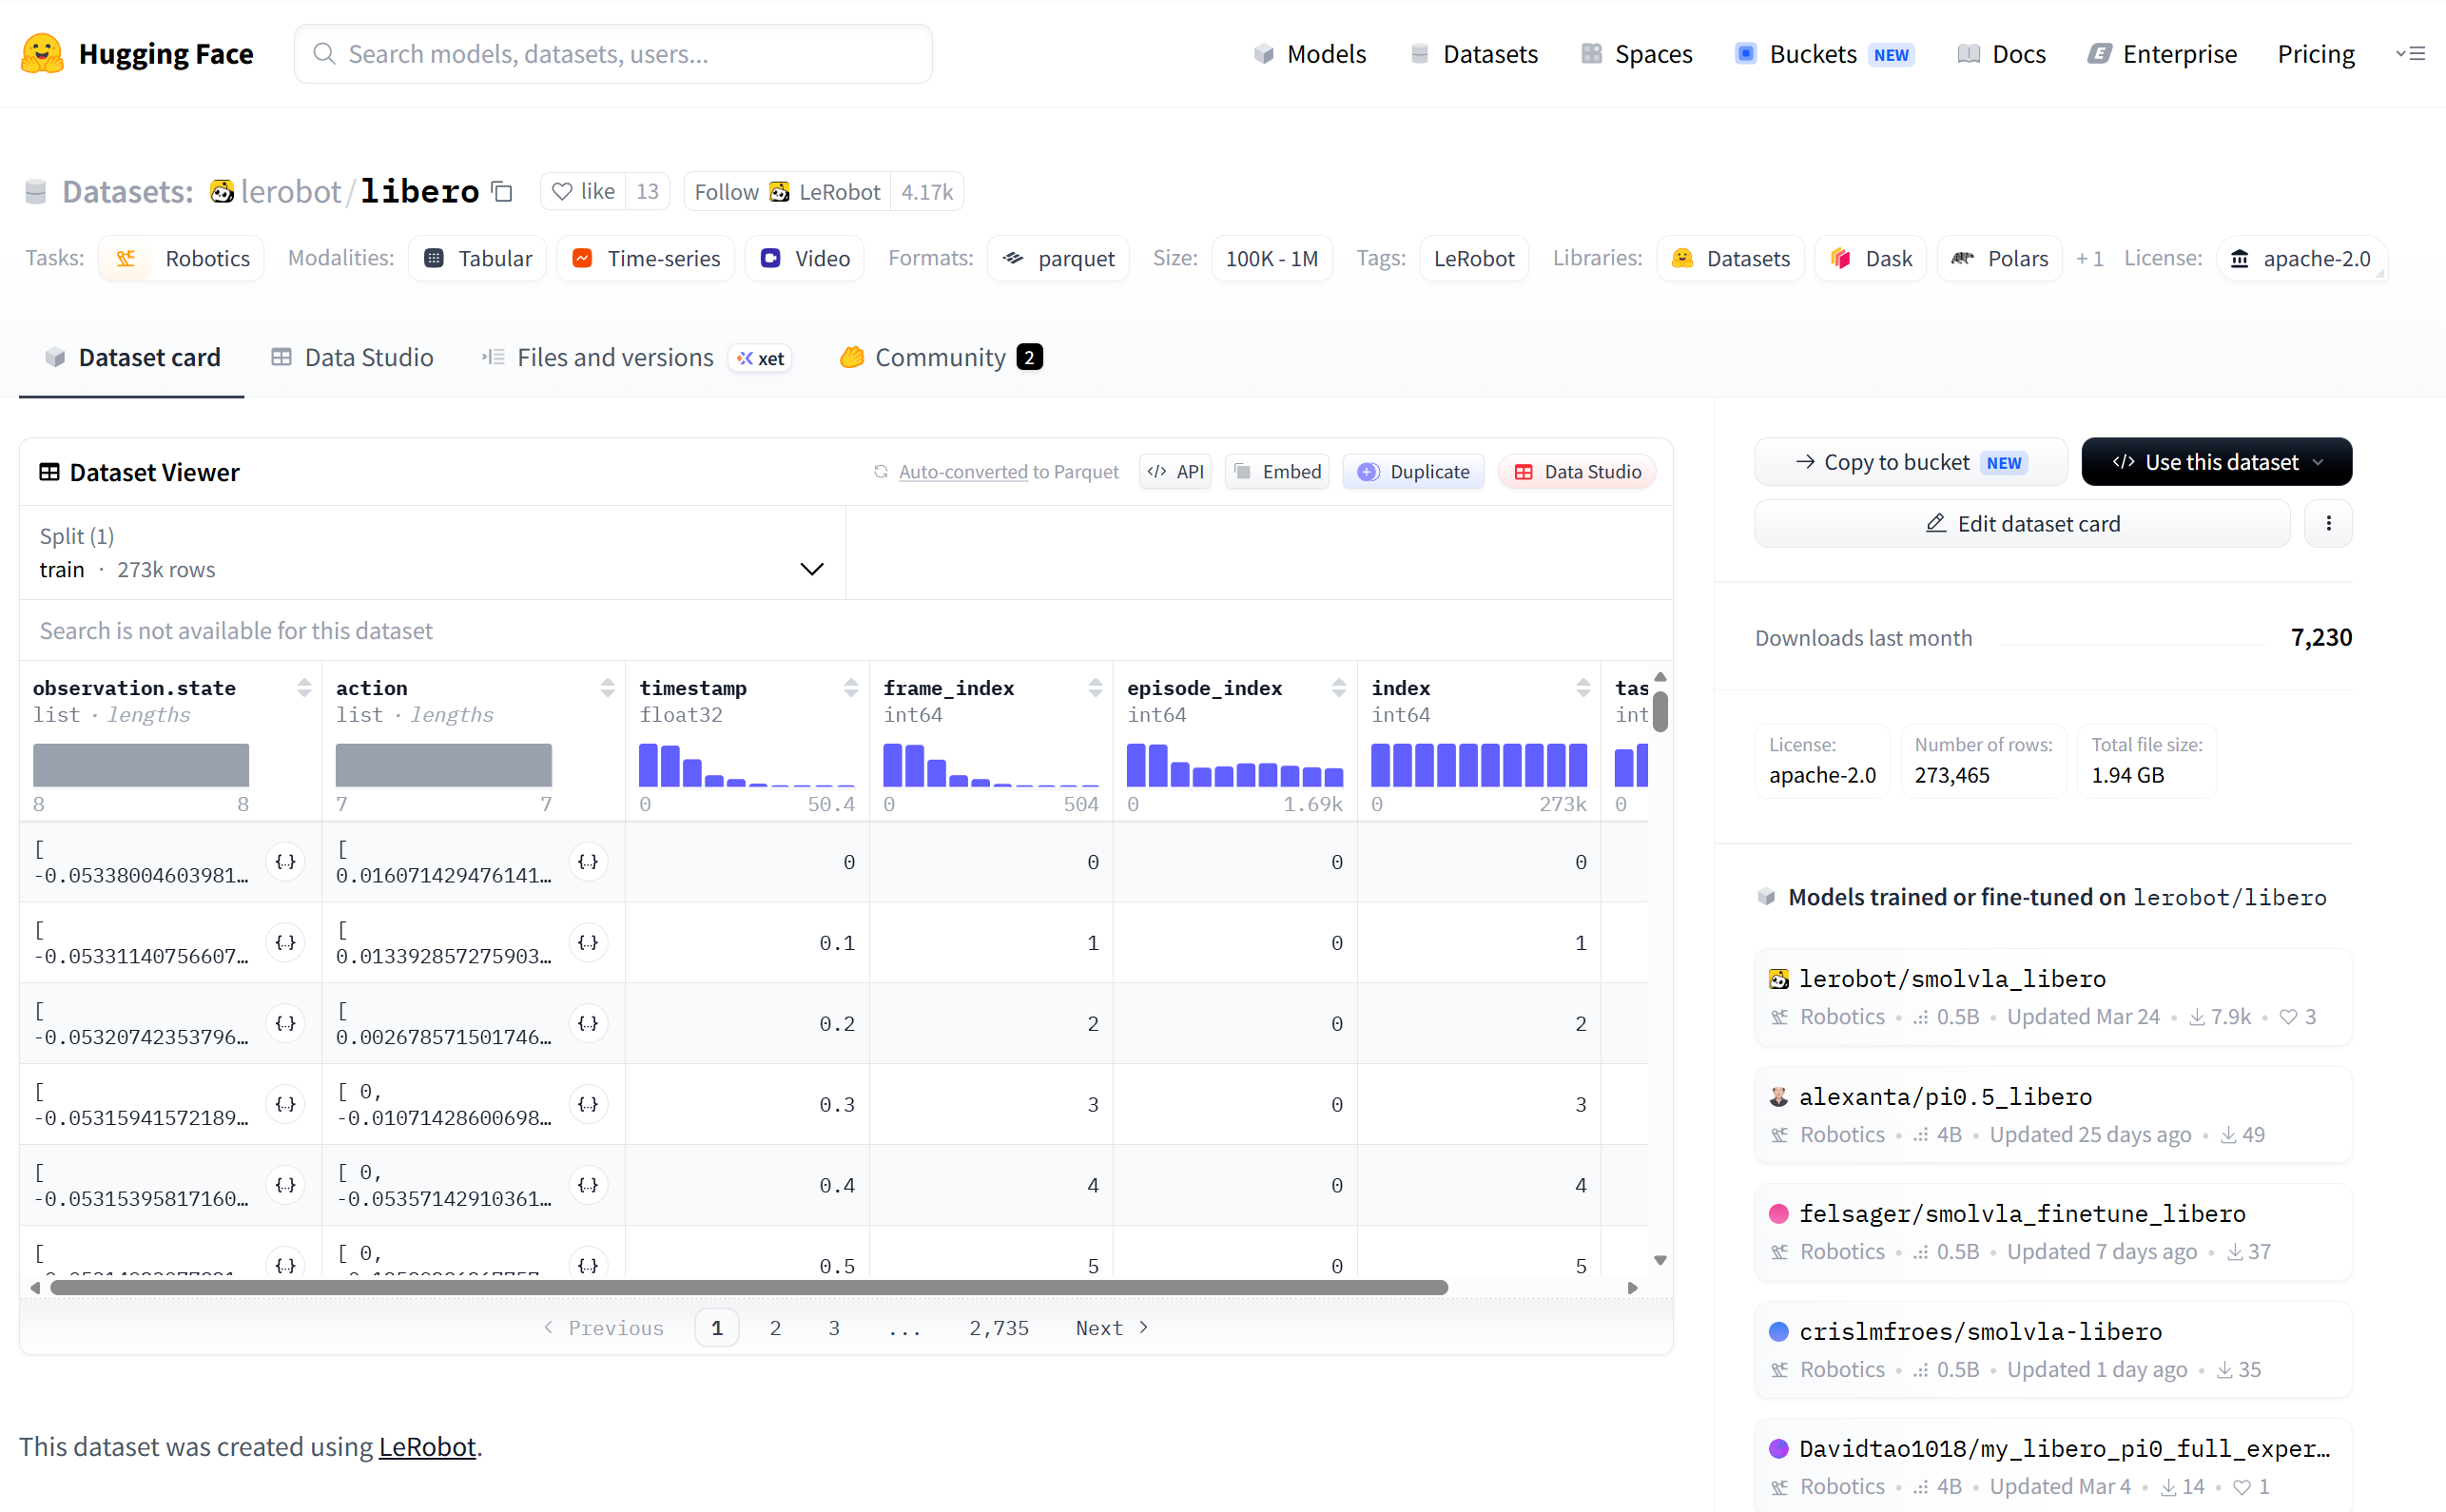
\includegraphics[width=0.98\linewidth,height=\textheight,keepaspectratio]{../../assets/figures/lecture09/ref/figures/fig93-libero-homepage.png}

}

\caption{lerobot/libero 数据集主页，顶部四个 tab
对应四种看法，右侧是行数 / 体积 / 月下载量与''谁在用它''}

\end{figure}%

打开一个 HF 数据集页面，顶部四个 tab 正好对应四种看法：

\begin{itemize}
\tightlist
\item
  \textbf{Dataset
  card}：概览页（标签、统计、自动生成的数据卡、谁在用它）。
\item
  \textbf{Data Studio}：内置表格浏览器，\textbf{无需下载}就能逐行翻看
  parquet（这里 273k 行分 2,735 页）。
\item
  \textbf{Files and versions}：物理文件树 + git 式版本历史（见 3.4.3）。
\item
  \textbf{Community}：讨论区。
\end{itemize}

顶部那排\textbf{标签}本身就是一张''身份证''：

\begin{center}
\begin{tabular}{@{}>{\raggedright\arraybackslash}p{\dimexpr 0.4289\linewidth - 2\tabcolsep\relax} >{\raggedright\arraybackslash}p{\dimexpr 0.5711\linewidth - 2\tabcolsep\relax}@{}}
\toprule\noalign{}
标签 & 含义 \\
\midrule\noalign{}
\texttt{Robotics} & 任务领域 \\
\texttt{Tabular} · \texttt{Time-series} · \texttt{Video} & 三种模态：表格（状态 / 动作）+ 时序 + 视频 \\
\texttt{parquet} & 底层存储格式 \\
\texttt{100K\ -\ 1M} & 行数量级（这里 27 万行） \\
\texttt{Dask} · \texttt{Polars} & 可直接用这些库流式查询 \\
\texttt{apache-2.0} & 许可证 \\
\bottomrule\noalign{}
\end{tabular}
\end{center}

右侧关键数字：\textbf{273,465 行 · 1.94 GB · 月下载约
7,230}------一个被大量真实使用的小型标准数据集。

\subsubsection{3.4.2 谁在用它：数据集 →
模型的生态闭环}\label{ux8c01ux5728ux7528ux5b83ux6570ux636eux96c6-ux6a21ux578bux7684ux751fux6001ux95edux73af}

Dataset card 右侧的 \textbf{``Models trained or fine-tuned on
lerobot/libero''}
列出了一串模型：\texttt{lerobot/smolvla\_libero}、\texttt{alexanta/pi0.5\_libero}、\texttt{felsager/smolvla\_finetune\_libero}、\texttt{crislmfroes/smolvla\_libero}\ldots\ldots{}

这正好呼应 3.1 那张闭环图：\textbf{同一份数据集，喂给
SmolVLA、\(\pi_{0.5}\) 等不同策略，就训出 /
微调出一批模型}。数据在下游沉淀为能力------这就是第 1
节''数据决定上限''最直观的体现。

\subsubsection{3.4.3 物理视角：Files and
versions}\label{ux7269ux7406ux89c6ux89d2files-and-versions}

切到 Files 这个 tab，看到的是\textbf{磁盘上真实的样子}，正好印证 3.3
的目录结构：

\begin{figure}[H]

{\centering 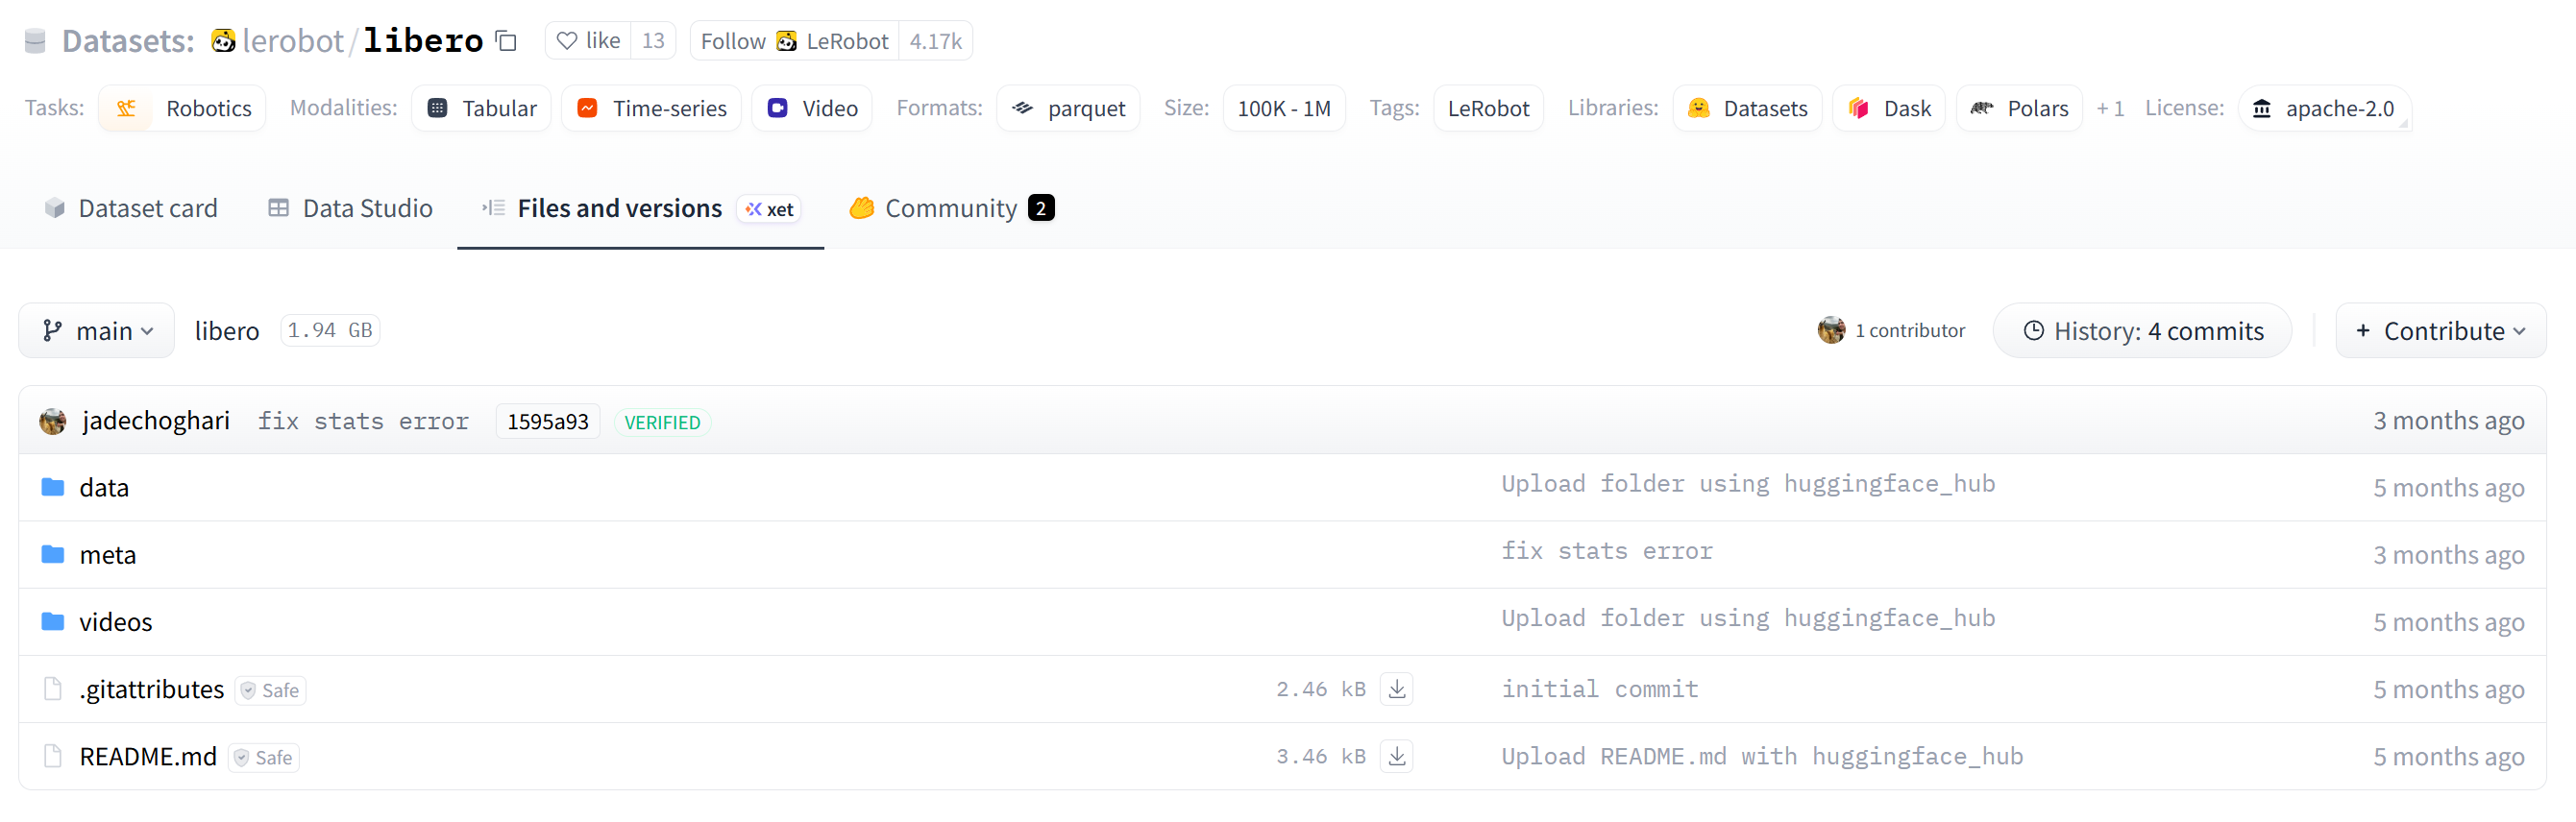
\includegraphics[width=0.98\linewidth,height=\textheight,keepaspectratio]{../../assets/figures/lecture09/ref/figures/fig93-libero-files.png}

}

\caption{Files and versions 文件树，三个顶层目录 data/ meta/ videos/
加上 git 式的 commit 历史}

\end{figure}%

\dirtree{%
.1 \texttt{libero/} {\color{TreeNoteColor}（1.94 GB，main 分支）}.
.2 \texttt{data/} {\color{TreeNoteColor}（表格数据 parquet）}.
.2 \texttt{meta/} {\color{TreeNoteColor}（元数据 info.json / stats / tasks / episodes）}.
.2 \texttt{videos/} {\color{TreeNoteColor}（多相机视频 mp4）}.
.2 \texttt{.gitattributes}.
.2 \texttt{README.md}.
}

三个顶层目录 \texttt{data/\ meta/\ videos/} 就是三大支柱的物理落地。HF
数据集本质是一个\textbf{带版本管理的 git 仓库}：页面记录了完整的 commit
历史（如
\texttt{fix\ stats\ error}），可以像代码一样回溯、追踪每一次改动。

\subsubsection{3.4.4 逻辑视角：Data Studio
逐行看数据}\label{ux903bux8f91ux89c6ux89d2data-studio-ux9010ux884cux770bux6570ux636e}

\begin{figure}[H]

{\centering 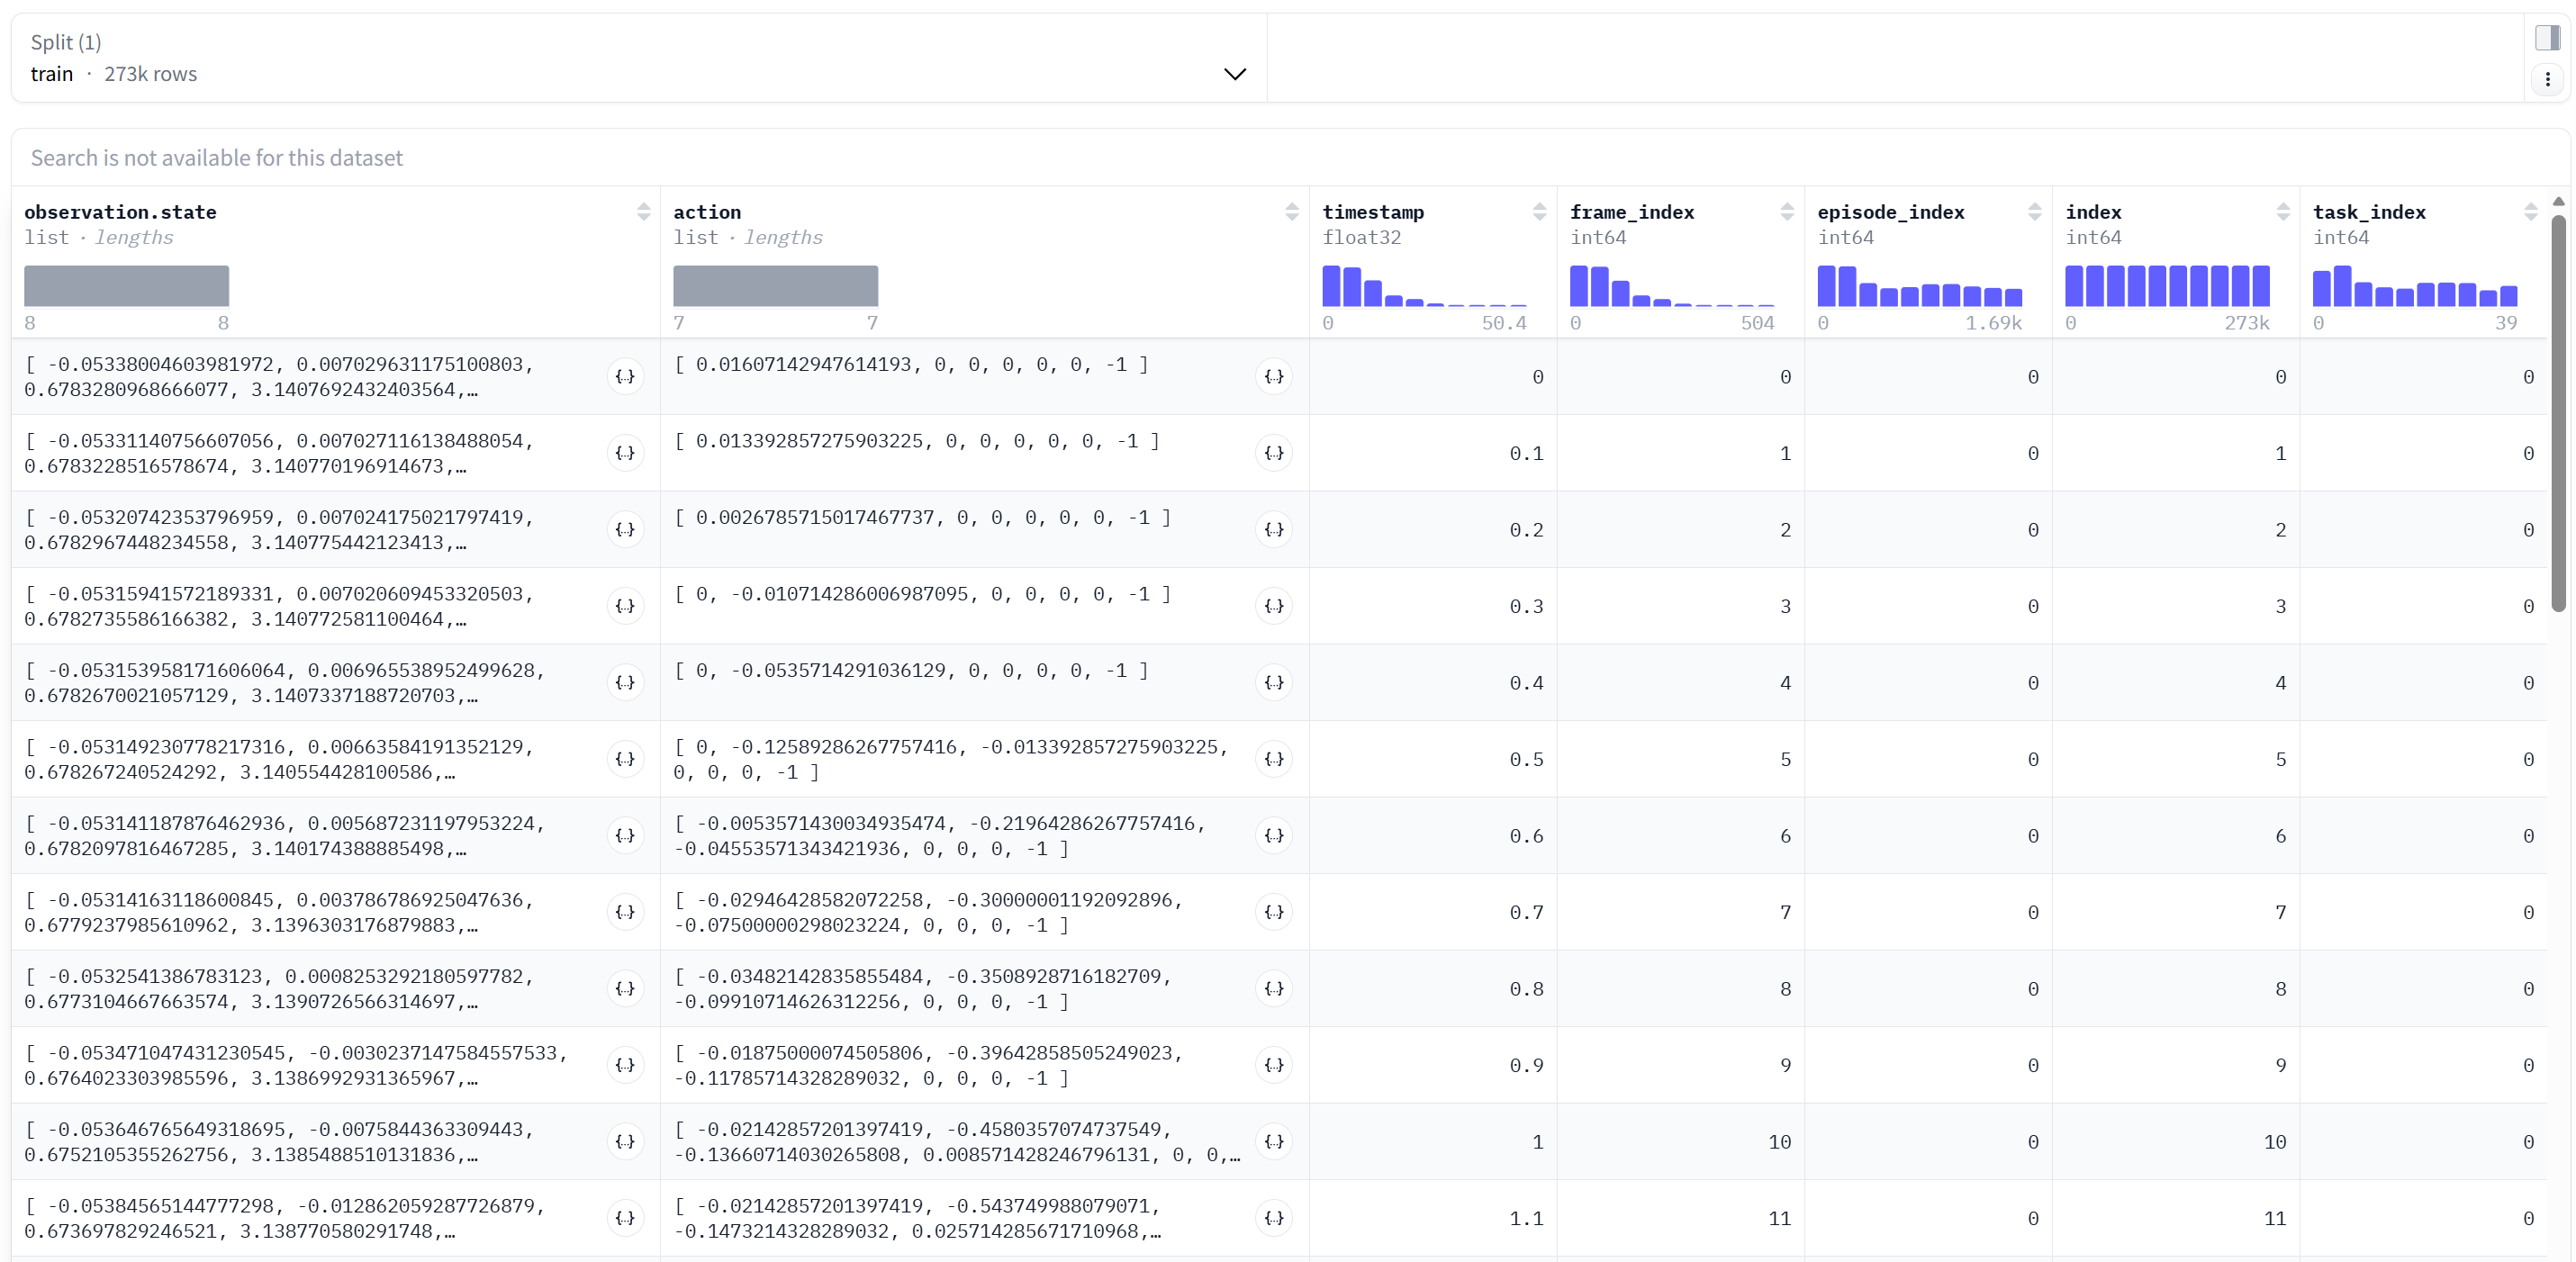
\includegraphics[width=0.98\linewidth,height=\textheight,keepaspectratio]{../../assets/figures/lecture09/ref/figures/fig93-libero-data-studio.png}

}

\caption{Data Studio 逐行浏览，把 parquet 一行一行摊开，每行是某 episode
在某时刻的一帧}

\end{figure}%

Data Studio 把 parquet 一行一行摊开，每一行 = 某个 episode
在某一时刻的一帧，重点看这几列：

\begin{itemize}
\tightlist
\item
  \textbf{\texttt{observation.state}}：长度 8
  的浮点数组------机器人\textbf{自身的本体感知}（关节角度 +
  夹爪），即''机器人感受到的身体状态''。
\item
  \textbf{\texttt{action}}：长度 7
  的浮点数组------该时刻\textbf{要下发执行的目标动作}；策略要学的，就是''看到
  state + 图像 → 输出 action''。
\item
  \textbf{三个 index 列的相对 vs 绝对语义}（看直方图分布最直观）：
\end{itemize}

\begin{center}
\begin{tabular}{@{}>{\raggedright\arraybackslash}p{\dimexpr 0.2071\linewidth - 2\tabcolsep\relax} >{\raggedright\arraybackslash}p{\dimexpr 0.6102\linewidth - 2\tabcolsep\relax} >{\raggedright\arraybackslash}p{\dimexpr 0.1827\linewidth - 2\tabcolsep\relax}@{}}
\toprule\noalign{}
列 & 语义 & 取值范围 \\
\midrule\noalign{}
\texttt{frame\_\allowbreak index} & \textbf{相对}：episode 内第几帧，每个 episode 从 0 重置 & 0 → \textasciitilde504 \\
\texttt{episode\_\allowbreak index} & 第几个 episode & 0 → 1,692 \\
\texttt{index} & \textbf{绝对}：全局第几帧，跨 episode 一直累积 & 0 → 273,464 \\
\texttt{task\_\allowbreak index} & 第几个任务（40 个之一） & 0 → 39 \\
\bottomrule\noalign{}
\end{tabular}
\end{center}

\begin{quote}
备注：\texttt{action} 与 \texttt{state}
的来源随\textbf{采集方式}而不同------本课的 SO-101
是\textbf{真机遥操作}，\texttt{action}
来自\textbf{主臂（leader）}、\texttt{state}
来自\textbf{从臂（follower）}，action 背后其实是人的操作意图；而
lerobot/libero 是\textbf{仿真}采集（Franka Panda in
LIBERO），没有人手主臂，\texttt{action} 是策略 /
脚本下发的目标动作。采集方式不同，落盘格式却完全一样------这正是统一格式的价值。
\end{quote}

认清了一份真实公开数据集长什么样，下面回到本课自己的 SO-101
采集，把一帧、一份说明书逐字段看穿。

\subsection{3.5
一帧数据里有什么}\label{ux4e00ux5e27ux6570ux636eux91ccux6709ux4ec0ux4e48}

把数据集里的一个样本（一帧）展开，返回的就是一个 Python 字典（值为
PyTorch 张量），这正是第8讲讲过的''观测 →
动作''配对，只是现在有了具体字段和形状。以本课 SO-101 双相机采集为例：

\begin{Shaded}
\begin{Highlighting}[]
\NormalTok{sample }\OperatorTok{=}\NormalTok{ dataset[}\DecValTok{100}\NormalTok{]}
\CommentTok{\# \{}
\CommentTok{\#   \textquotesingle{}observation.images.front\textquotesingle{}: tensor([3, 480, 640]),  \# 前视相机，CHW}
\CommentTok{\#   \textquotesingle{}observation.images.side\textquotesingle{}:  tensor([3, 480, 640]),  \# 侧视相机}
\CommentTok{\#   \textquotesingle{}observation.state\textquotesingle{}:        tensor([6]),            \# 本体感知：6 个关节读数}
\CommentTok{\#   \textquotesingle{}action\textquotesingle{}:                   tensor([6]),            \# 动作：6 个关节目标（含夹爪）}
\CommentTok{\#   \textquotesingle{}timestamp\textquotesingle{}:                tensor(3.3),            \# 秒}
\CommentTok{\#   \textquotesingle{}frame\_index\textquotesingle{}:              tensor(99),             \# episode 内帧索引}
\CommentTok{\#   \textquotesingle{}episode\_index\textquotesingle{}:            tensor(0),              \# 第几个 episode}
\CommentTok{\#   \textquotesingle{}index\textquotesingle{}:                    tensor(100),            \# 全局帧索引（跨 episode 累积）}
\CommentTok{\#   \textquotesingle{}task\_index\textquotesingle{}:               tensor(0),              \# 第几个任务}
\CommentTok{\#   \textquotesingle{}task\textquotesingle{}: "Put the cuboid into the basket"            \# 自然语言任务描述}
\CommentTok{\# \}}
\end{Highlighting}
\end{Shaded}

这里有两个细节值得点破：

\begin{quote}
备注：列里看不到「图像」本身------图像存在 \texttt{videos/} 的 mp4
里。取样本时，LeRobotDataset 用这一帧的 \texttt{timestamp}
去对应视频里\textbf{按时间解码出那一帧}，再和表格数据拼成一个完整样本。

备注：\texttt{frame\_index} 是\textbf{相对}索引（每个 episode 从 0
重置），\texttt{index} 是\textbf{绝对}索引（跨 episode
一直累积）；\texttt{observation.state}
是机器人\textbf{自己的关节读数}（部分可观测的观测，不是环境真实状态），\texttt{action}
是该时刻\textbf{要下发执行的目标动作}------策略要学的，就是「看到 state
+ 图像 → 输出 action」。
\end{quote}

\subsection{3.6
info.json：数据集的「说明书」}\label{info.jsonux6570ux636eux96c6ux7684ux8bf4ux660eux4e66}

\texttt{meta/info.json} 是整份数据集的 schema
真相来源，一份采集的所有口径都写在这里。下面是 SO-101 cuboid 采集的
info.json 骨架（\texttt{side} 相机与 \texttt{front} 结构相同，省略）：

\begin{Shaded}
\begin{Highlighting}[]
\FunctionTok{\{}
  \DataTypeTok{"codebase\_version"}\FunctionTok{:} \StringTok{"v3.0"}\FunctionTok{,}
  \DataTypeTok{"robot\_type"}\FunctionTok{:} \StringTok{"so101\_follower"}\FunctionTok{,}
  \DataTypeTok{"total\_episodes"}\FunctionTok{:} \DecValTok{50}\FunctionTok{,}
  \DataTypeTok{"total\_frames"}\FunctionTok{:} \DecValTok{45000}\FunctionTok{,}
  \DataTypeTok{"total\_tasks"}\FunctionTok{:} \DecValTok{1}\FunctionTok{,}
  \DataTypeTok{"fps"}\FunctionTok{:} \DecValTok{30}\FunctionTok{,}
  \DataTypeTok{"data\_path"}\FunctionTok{:}  \StringTok{"data/chunk{-}\{chunk\_index:03d\}/file{-}\{file\_index:03d\}.parquet"}\FunctionTok{,}
  \DataTypeTok{"video\_path"}\FunctionTok{:} \StringTok{"videos/\{video\_key\}/chunk{-}\{chunk\_index:03d\}/file{-}\{file\_index:03d\}.mp4"}\FunctionTok{,}
  \DataTypeTok{"features"}\FunctionTok{:} \FunctionTok{\{}
    \DataTypeTok{"observation.images.front"}\FunctionTok{:} \FunctionTok{\{}
      \DataTypeTok{"dtype"}\FunctionTok{:} \StringTok{"video"}\FunctionTok{,}
      \DataTypeTok{"shape"}\FunctionTok{:} \OtherTok{[}\DecValTok{480}\OtherTok{,} \DecValTok{640}\OtherTok{,} \DecValTok{3}\OtherTok{]}\FunctionTok{,}
      \DataTypeTok{"names"}\FunctionTok{:} \OtherTok{[}\StringTok{"height"}\OtherTok{,} \StringTok{"width"}\OtherTok{,} \StringTok{"channel"}\OtherTok{]}\FunctionTok{,}
      \DataTypeTok{"info"}\FunctionTok{:} \FunctionTok{\{} \DataTypeTok{"video.codec"}\FunctionTok{:} \StringTok{"av1"}\FunctionTok{,} \DataTypeTok{"video.fps"}\FunctionTok{:} \DecValTok{30}\FunctionTok{,} \DataTypeTok{"video.is\_depth\_map"}\FunctionTok{:} \KeywordTok{false} \FunctionTok{\}}
    \FunctionTok{\},}
    \DataTypeTok{"observation.images.side"}\FunctionTok{:} \FunctionTok{\{} \DataTypeTok{"..."}\FunctionTok{:} \StringTok{"同上（侧视相机）"} \FunctionTok{\},}
    \DataTypeTok{"observation.state"}\FunctionTok{:} \FunctionTok{\{} \DataTypeTok{"dtype"}\FunctionTok{:} \StringTok{"float32"}\FunctionTok{,} \DataTypeTok{"shape"}\FunctionTok{:} \OtherTok{[}\DecValTok{6}\OtherTok{]}\FunctionTok{,} \DataTypeTok{"names"}\FunctionTok{:} \OtherTok{[}\StringTok{"state"}\OtherTok{]} \FunctionTok{\},}
    \DataTypeTok{"action"}\FunctionTok{:}            \FunctionTok{\{} \DataTypeTok{"dtype"}\FunctionTok{:} \StringTok{"float32"}\FunctionTok{,} \DataTypeTok{"shape"}\FunctionTok{:} \OtherTok{[}\DecValTok{6}\OtherTok{]}\FunctionTok{,} \DataTypeTok{"names"}\FunctionTok{:} \OtherTok{[}\StringTok{"action"}\OtherTok{]} \FunctionTok{\},}
    \DataTypeTok{"timestamp"}\FunctionTok{:}     \FunctionTok{\{} \DataTypeTok{"dtype"}\FunctionTok{:} \StringTok{"float32"}\FunctionTok{,} \DataTypeTok{"shape"}\FunctionTok{:} \OtherTok{[}\DecValTok{1}\OtherTok{]}\FunctionTok{,} \DataTypeTok{"names"}\FunctionTok{:} \KeywordTok{null} \FunctionTok{\},}
    \DataTypeTok{"frame\_index"}\FunctionTok{:}   \FunctionTok{\{} \DataTypeTok{"dtype"}\FunctionTok{:} \StringTok{"int64"}\FunctionTok{,}   \DataTypeTok{"shape"}\FunctionTok{:} \OtherTok{[}\DecValTok{1}\OtherTok{]}\FunctionTok{,} \DataTypeTok{"names"}\FunctionTok{:} \KeywordTok{null} \FunctionTok{\},}
    \DataTypeTok{"episode\_index"}\FunctionTok{:} \FunctionTok{\{} \DataTypeTok{"dtype"}\FunctionTok{:} \StringTok{"int64"}\FunctionTok{,}   \DataTypeTok{"shape"}\FunctionTok{:} \OtherTok{[}\DecValTok{1}\OtherTok{]}\FunctionTok{,} \DataTypeTok{"names"}\FunctionTok{:} \KeywordTok{null} \FunctionTok{\},}
    \DataTypeTok{"index"}\FunctionTok{:}         \FunctionTok{\{} \DataTypeTok{"dtype"}\FunctionTok{:} \StringTok{"int64"}\FunctionTok{,}   \DataTypeTok{"shape"}\FunctionTok{:} \OtherTok{[}\DecValTok{1}\OtherTok{]}\FunctionTok{,} \DataTypeTok{"names"}\FunctionTok{:} \KeywordTok{null} \FunctionTok{\},}
    \DataTypeTok{"task\_index"}\FunctionTok{:}    \FunctionTok{\{} \DataTypeTok{"dtype"}\FunctionTok{:} \StringTok{"int64"}\FunctionTok{,}   \DataTypeTok{"shape"}\FunctionTok{:} \OtherTok{[}\DecValTok{1}\OtherTok{]}\FunctionTok{,} \DataTypeTok{"names"}\FunctionTok{:} \KeywordTok{null} \FunctionTok{\}}
  \FunctionTok{\}}
\FunctionTok{\}}
\end{Highlighting}
\end{Shaded}

逐字段读这份说明书：顶层是\textbf{数据集级}口径------\texttt{robot\_type}
机器人型号、\texttt{total\_episodes/frames/tasks} 规模、\texttt{fps}
采样帧率、\texttt{data\_path}/\texttt{video\_path}
是\textbf{路径模板}（把
\texttt{chunk\_index}、\texttt{file\_index}、\texttt{video\_key}
填进去就拼出真实文件路径）。\texttt{features} 里每个字段声明
\texttt{dtype}（\texttt{video} 走 mp4 / \texttt{float32} /
\texttt{int64}）、\texttt{shape}（维度，图像
\texttt{{[}480,640,3{]}}、状态 \texttt{{[}6{]}}、动作
\texttt{{[}6{]}}）、\texttt{names}（每维名字），video
字段还附编码细节（\texttt{av1} 编码、\texttt{is\_depth\_map=false}
表示是 RGB 不是深度图）。\textbf{读懂
info.json，就读懂了一份数据集的全部口径。}

\subsection{3.7
加载、切时间窗与可视化回看}\label{ux52a0ux8f7dux5207ux65f6ux95f4ux7a97ux4e0eux53efux89c6ux5316ux56deux770b}

落盘之后，训练侧主要做三件事，LeRobot 都封装成了简洁的 API。

\textbf{一、加载数据集。} 从 Hub 或本地一行加载，可只取部分 episode
省内存，也能不下载直接流式读取：

\begin{Shaded}
\begin{Highlighting}[]
\ImportTok{from}\NormalTok{ lerobot.datasets.lerobot\_dataset }\ImportTok{import}\NormalTok{ LeRobotDataset}

\NormalTok{dataset }\OperatorTok{=}\NormalTok{ LeRobotDataset(}\StringTok{"local/cuboid"}\NormalTok{)            }\CommentTok{\# 加载（自动缓存）}
\BuiltInTok{print}\NormalTok{(dataset.meta.total\_episodes, dataset.meta.fps)  }\CommentTok{\# 看元信息}
\NormalTok{dataset }\OperatorTok{=}\NormalTok{ LeRobotDataset(}\StringTok{"local/cuboid"}\NormalTok{, episodes}\OperatorTok{=}\NormalTok{[}\DecValTok{0}\NormalTok{, }\DecValTok{1}\NormalTok{, }\DecValTok{2}\NormalTok{])  }\CommentTok{\# 只取前 3 个 episode}
\NormalTok{sample }\OperatorTok{=}\NormalTok{ dataset[}\DecValTok{100}\NormalTok{]                               }\CommentTok{\# 随机访问一帧}
\end{Highlighting}
\end{Shaded}

\textbf{二、切时间窗（delta\_timestamps）。}
很多策略不是只看「当前这一帧」就够：有的要把过去若干帧拼起来看运动趋势，有的要一次输出未来几十帧动作（\textbf{action
chunk}，如 50 帧 \(\approx\) 1.6
s，让灵巧操作更连贯）。\texttt{delta\_timestamps}
就是取样本时顺带把「相对当前帧的前后若干时刻」一起按时间对齐取出、堆成带时间维的张量：

\begin{Shaded}
\begin{Highlighting}[]
\CommentTok{\# 取当前帧及前 0.2s、0.1s 的前视图像（历史上下文）}
\NormalTok{delta\_timestamps }\OperatorTok{=}\NormalTok{ \{}\StringTok{"observation.images.front"}\NormalTok{: [}\OperatorTok{{-}}\FloatTok{0.2}\NormalTok{, }\OperatorTok{{-}}\FloatTok{0.1}\NormalTok{, }\FloatTok{0.0}\NormalTok{]\}}
\NormalTok{dataset }\OperatorTok{=}\NormalTok{ LeRobotDataset(}\StringTok{"local/cuboid"}\NormalTok{, delta\_timestamps}\OperatorTok{=}\NormalTok{delta\_timestamps)}
\BuiltInTok{print}\NormalTok{(dataset[}\DecValTok{100}\NormalTok{][}\StringTok{"observation.images.front"}\NormalTok{].shape)  }\CommentTok{\# [3, 3, 480, 640]，T=3}
\end{Highlighting}
\end{Shaded}

\textbf{三、可视化回看。} 把某条 episode
的图像与各维动作、状态曲线逐帧放出来，肉眼检查这条数据采得干不干净------这又回到质量这件事上。两条路：在线用
HuggingFace Spaces 的
\texttt{visualize\_dataset}（无需下载、浏览器直接看），本地用基于 Rerun
的可视化工具：

\begin{Shaded}
\begin{Highlighting}[]
\ExtensionTok{lerobot{-}dataset{-}viz} \AttributeTok{{-}{-}repo{-}id}\NormalTok{ local/cuboid }\AttributeTok{{-}{-}episode{-}index}\NormalTok{ 0}
\end{Highlighting}
\end{Shaded}

Rerun 里能同步看到多相机图像、动作各维曲线、本体状态各维曲线，并支持按帧
/ 按时间戳导航。

\textbf{四、喂进训练（DataLoader）。} LeRobotDataset 就是标准的 PyTorch
\texttt{Dataset}，直接套 \texttt{DataLoader} 就能批量喂给模型：

\begin{Shaded}
\begin{Highlighting}[]
\ImportTok{import}\NormalTok{ torch}

\NormalTok{dataloader }\OperatorTok{=}\NormalTok{ torch.utils.data.DataLoader(dataset, batch\_size}\OperatorTok{=}\DecValTok{16}\NormalTok{, shuffle}\OperatorTok{=}\VariableTok{True}\NormalTok{, num\_workers}\OperatorTok{=}\DecValTok{4}\NormalTok{)}
\ControlFlowTok{for}\NormalTok{ batch }\KeywordTok{in}\NormalTok{ dataloader:}
\NormalTok{    states  }\OperatorTok{=}\NormalTok{ batch[}\StringTok{"observation.state"}\NormalTok{]          }\CommentTok{\# [B, 6]}
\NormalTok{    actions }\OperatorTok{=}\NormalTok{ batch[}\StringTok{"action"}\NormalTok{]                     }\CommentTok{\# [B, 6]}
\NormalTok{    images  }\OperatorTok{=}\NormalTok{ batch[}\StringTok{"observation.images.front"}\NormalTok{]   }\CommentTok{\# [B, 3, 480, 640]}
    \CommentTok{\# model.forward(batch) ...}
\end{Highlighting}
\end{Shaded}

\textbf{五、流式读取（无需下载）。} 数据集很大、本地放不下时，用
\texttt{StreamingLeRobotDataset} 直接从 Hub 边下边读，不占本地磁盘：

\begin{Shaded}
\begin{Highlighting}[]
\ImportTok{from}\NormalTok{ lerobot.datasets.streaming\_dataset }\ImportTok{import}\NormalTok{ StreamingLeRobotDataset}

\NormalTok{dataset }\OperatorTok{=}\NormalTok{ StreamingLeRobotDataset(}\StringTok{"lerobot/libero"}\NormalTok{)}
\ControlFlowTok{for}\NormalTok{ sample }\KeywordTok{in}\NormalTok{ dataset:}
    \BuiltInTok{print}\NormalTok{(sample[}\StringTok{"action"}\NormalTok{])}\OperatorTok{;} \ControlFlowTok{break}
\end{Highlighting}
\end{Shaded}

\textbf{六、数据增强（可选）。} 训练时常对图像做随机增强（亮度 /
对比度抖动等），LeRobot 内置 \texttt{ImageTransforms}，作为
\texttt{image\_transforms} 传入即可，落盘数据本身不动。

最后给一张''想改源码时去哪找''的速查表，\texttt{lerobot/datasets/}
下与本讲相关的关键文件（\textbf{与版本相关}，按上文的 0.4.0 / v3.0
口径记录；新版本里文件可能改名或拆分，找不到就直接在源码树里搜类名）：

\begin{center}
\begin{tabular}{@{}>{\raggedright\arraybackslash}p{\dimexpr 0.2861\linewidth - 2\tabcolsep\relax} >{\raggedright\arraybackslash}p{\dimexpr 0.7139\linewidth - 2\tabcolsep\relax}@{}}
\toprule\noalign{}
文件 & 作用 \\
\midrule\noalign{}
\texttt{lerobot\_\allowbreak dataset.py} & 核心类 \texttt{LeRobotDataset} / \texttt{LeRobotDatasetMetadata} / \texttt{MultiLeRobotDataset} \\
\texttt{streaming\_\allowbreak dataset.py} & \texttt{StreamingLeRobotDataset}（流式读取） \\
\texttt{video\_\allowbreak utils.py} & 视频编解码（torchcodec / pyav） \\
\texttt{transforms.py} & 图像数据增强 \\
\texttt{compute\_\allowbreak stats.py} & 计算数据集统计（mean/std），写 \texttt{stats.json} \\
\texttt{factory.py} & \texttt{make\_\allowbreak dataset()}：从训练配置创建数据集 \\
\texttt{lerobot\_\allowbreak dataset\_\allowbreak viz.py} & 本地可视化（Rerun） \\
\bottomrule\noalign{}
\end{tabular}
\end{center}

认全了格式，下一节就回到「采」这件事：用最小的 SO-101
把一条数据采出来，看它怎么长成上面这套结构。

\section{4
实验：采一段抓取数据}\label{ux5b9eux9a8cux91c7ux4e00ux6bb5ux6293ux53d6ux6570ux636e}

理论与格式都铺完了，这一节动手采一段''把方块放进篮子''的数据，把第 2
节的主从臂方案跑成一份真实落盘的 LeRobotDataset。

\subsection{4.1 实物方案：SO-101
主从臂}\label{ux5b9eux7269ux65b9ux6848so-101-ux4e3bux4eceux81c2}

实物方案用一对 SO-101 主从臂。它俩\textbf{结构完全同构}------都是 6 个
Feetech
舵机（\texttt{shoulder\_pan\ /\ shoulder\_lift\ /\ elbow\_flex\ /\ wrist\_flex\ /\ wrist\_roll\ /\ gripper}）。正因为同构，在\textbf{逐关节标定过、方向与量程都核对过}的前提下，主臂读到的关节角度可以逐关节映射成从臂的目标角度，这就是主从遥操作能成立的根本：

\begin{itemize}
\tightlist
\item
  人手扳动 \textbf{leader 主臂}，\textbf{follower
  从臂}实时跟随做出同样的动作；
\item
  主臂当前的关节角度，就是这一帧的\textbf{动作标签}
  \texttt{action}（人想让机械臂去的地方）；
\item
  从臂自身的关节读数 + 机位相机画面，就是这一帧的\textbf{观测}
  \texttt{observation}。
\end{itemize}

于是人只要专注地用主臂把任务做一遍，\textbf{观测和动作标签就被同时、自动地配好对}。采集流程分两步走：先把遥操作本身跑通，再在遥操作之上开启录制。这两步对应
LeRobot 自带的两条命令------\texttt{lerobot-teleoperate} 和
\texttt{lerobot-record}。

\subsection{4.2
第一步：先跑通遥操作（lerobot-teleoperate）}\label{ux7b2cux4e00ux6b65ux5148ux8dd1ux901aux9065ux64cdux4f5clerobot-teleoperate}

正式录之前，先用 \texttt{lerobot-teleoperate}
验证整套硬件------主臂扳动时从臂方向对不对、相机有没有画面、帧率稳不稳：

\begin{Shaded}
\begin{Highlighting}[]
\ExtensionTok{lerobot{-}teleoperate} \DataTypeTok{\textbackslash{}}
    \AttributeTok{{-}{-}robot.type}\OperatorTok{=}\NormalTok{so101\_follower }\DataTypeTok{\textbackslash{}}
    \AttributeTok{{-}{-}robot.port}\OperatorTok{=}\NormalTok{/dev/ttyFollower }\DataTypeTok{\textbackslash{}}
    \AttributeTok{{-}{-}robot.id}\OperatorTok{=}\NormalTok{my\_follower\_arm }\DataTypeTok{\textbackslash{}}
    \AttributeTok{{-}{-}robot.cameras}\OperatorTok{=}\StringTok{\textquotesingle{}\{}
\StringTok{        front: \{type: opencv, index\_or\_path: 0, width: 640, height: 480, fps: 30\},}
\StringTok{        side:  \{type: opencv, index\_or\_path: 2, width: 640, height: 480, fps: 30\}}
\StringTok{      \}\textquotesingle{}} \DataTypeTok{\textbackslash{}}
    \AttributeTok{{-}{-}teleop.type}\OperatorTok{=}\NormalTok{so101\_leader }\DataTypeTok{\textbackslash{}}
    \AttributeTok{{-}{-}teleop.port}\OperatorTok{=}\NormalTok{/dev/ttyLeader }\DataTypeTok{\textbackslash{}}
    \AttributeTok{{-}{-}teleop.id}\OperatorTok{=}\NormalTok{my\_leader\_arm }\DataTypeTok{\textbackslash{}}
    \AttributeTok{{-}{-}display\_data}\OperatorTok{=}\NormalTok{true }\DataTypeTok{\textbackslash{}}
    \AttributeTok{{-}{-}fps}\OperatorTok{=}\NormalTok{30}
\end{Highlighting}
\end{Shaded}

参数其实只分三组------\textbf{从臂（\texttt{-\/-robot.*}）、主臂（\texttt{-\/-teleop.*}）、显示与帧率}：

\begin{center}
\begin{tabular}{@{}>{\raggedright\arraybackslash}p{\dimexpr 0.4688\linewidth - 2\tabcolsep\relax} >{\raggedright\arraybackslash}p{\dimexpr 0.5312\linewidth - 2\tabcolsep\relax}@{}}
\toprule\noalign{}
参数 & 含义 \\
\midrule\noalign{}
\texttt{-\/-robot.type=so101\_\allowbreak follower} & 从臂类型，决定加载哪个 Robot 类 \\
\texttt{-\/-robot.port=/dev/ttyFollower} & 从臂串口（udev 固定名） \\
\texttt{-\/-robot.id=...} & 从臂唯一名，用于找到它的标定文件 \\
\texttt{-\/-robot.cameras=...} & 相机配置：\texttt{front}（设备 0）+ \texttt{side}（设备 2），均 640×480@30 \\
\texttt{-\/-teleop.type=so101\_\allowbreak leader} & 主臂类型 \\
\texttt{-\/-teleop.port=/dev/ttyLeader} & 主臂串口（udev 固定名） \\
\texttt{-\/-teleop.id=...} & 主臂唯一名（对应主臂标定文件） \\
\texttt{-\/-display\_\allowbreak data=true} & 开实时显示，看相机画面与动作曲线 \\
\texttt{-\/-fps=30} & 控制环目标频率 30 Hz \\
\bottomrule\noalign{}
\end{tabular}
\end{center}

这一步只做「读主臂 → 写从臂」、不落盘，纯粹用来确认硬件正常。

\begin{quote}
备注：本演示假设主从臂已完成\textbf{标定}（把主从臂关节读数对齐到同一套零位与量程），且串口已用
udev 固定成
\texttt{/dev/ttyLeader}、\texttt{/dev/ttyFollower}。零位对齐之后，这套遥操作就是
2.2.2 说的\textbf{绝对跟踪}------录下的 \texttt{action}
是下发给从臂的目标角度，从臂实测到达的姿态记在
\texttt{observation.state} 里，两者会差一点跟踪误差。
\end{quote}

\subsection{4.3
第二步：在遥操作之上录数据（lerobot-record）}\label{ux7b2cux4e8cux6b65ux5728ux9065ux64cdux4f5cux4e4bux4e0aux5f55ux6570ux636elerobot-record}

硬件确认无误，把命令换成
\texttt{lerobot-record}------它干的事就是「遥操作」再加上「把每一帧写进数据集」。前半段（robot
/ teleop / cameras / display）和上一条\textbf{一模一样}，新增的全是
\texttt{-\/-dataset.*}：

\begin{Shaded}
\begin{Highlighting}[]
\ExtensionTok{lerobot{-}record} \DataTypeTok{\textbackslash{}}
    \AttributeTok{{-}{-}robot.type}\OperatorTok{=}\NormalTok{so101\_follower }\AttributeTok{{-}{-}robot.port}\OperatorTok{=}\NormalTok{/dev/ttyFollower }\AttributeTok{{-}{-}robot.id}\OperatorTok{=}\NormalTok{my\_follower\_arm }\DataTypeTok{\textbackslash{}}
    \AttributeTok{{-}{-}robot.cameras}\OperatorTok{=}\StringTok{\textquotesingle{}\{}
\StringTok{        front: \{type: opencv, index\_or\_path: 0, width: 640, height: 480, fps: 30\},}
\StringTok{        side:  \{type: opencv, index\_or\_path: 2, width: 640, height: 480, fps: 30\}}
\StringTok{      \}\textquotesingle{}} \DataTypeTok{\textbackslash{}}
    \AttributeTok{{-}{-}teleop.type}\OperatorTok{=}\NormalTok{so101\_leader }\AttributeTok{{-}{-}teleop.port}\OperatorTok{=}\NormalTok{/dev/ttyLeader }\AttributeTok{{-}{-}teleop.id}\OperatorTok{=}\NormalTok{my\_leader\_arm }\DataTypeTok{\textbackslash{}}
    \AttributeTok{{-}{-}display\_data}\OperatorTok{=}\NormalTok{true }\DataTypeTok{\textbackslash{}}
    \AttributeTok{{-}{-}fps}\OperatorTok{=}\NormalTok{30 }\DataTypeTok{\textbackslash{}}
    \AttributeTok{{-}{-}dataset.repo\_id}\OperatorTok{=}\NormalTok{local/cuboid }\DataTypeTok{\textbackslash{}}
    \AttributeTok{{-}{-}dataset.single\_task}\OperatorTok{=}\StringTok{"Put the cuboid into the basket"} \DataTypeTok{\textbackslash{}}
    \AttributeTok{{-}{-}dataset.num\_episodes}\OperatorTok{=}\NormalTok{50 }\DataTypeTok{\textbackslash{}}
    \AttributeTok{{-}{-}dataset.episode\_time\_s}\OperatorTok{=}\NormalTok{30 }\DataTypeTok{\textbackslash{}}
    \AttributeTok{{-}{-}dataset.reset\_time\_s}\OperatorTok{=}\NormalTok{30 }\DataTypeTok{\textbackslash{}}
    \AttributeTok{{-}{-}dataset.push\_to\_hub}\OperatorTok{=}\NormalTok{false}
\CommentTok{\#   {-}{-}resume=true}
\end{Highlighting}
\end{Shaded}

\begin{center}
\begin{tabular}{@{}>{\raggedright\arraybackslash}p{\dimexpr 0.3183\linewidth - 2\tabcolsep\relax} >{\raggedright\arraybackslash}p{\dimexpr 0.6817\linewidth - 2\tabcolsep\relax}@{}}
\toprule\noalign{}
\texttt{-\/-dataset.*} 参数 & 含义 \\
\midrule\noalign{}
\texttt{-\/-dataset.repo\_\allowbreak id=local/cuboid} & 数据集标识（\texttt{\textless{}namespace\textgreater{}/\textless{}name\textgreater{}} 形式），决定落盘目录名；上不上传由下面的 \texttt{push\_\allowbreak to\_\allowbreak hub} 决定，不由这里的 \texttt{local/} 决定 \\
\texttt{-\/-dataset.single\_\allowbreak task="..."} & 任务的自然语言描述，写进每一帧的 \texttt{task} 字段 \\
\texttt{-\/-dataset.num\_\allowbreak episodes=50} & 录 50 个回合（episode） \\
\texttt{-\/-dataset.episode\_\allowbreak time\_\allowbreak s=30} & 每个回合录 30 秒 \\
\texttt{-\/-dataset.reset\_\allowbreak time\_\allowbreak s=30} & 两个回合之间留 30 秒手动复位场景 \\
\texttt{-\/-dataset.push\_\allowbreak to\_\allowbreak hub=false} & 不上传到 HuggingFace Hub。这才是''离线开关''；要上传时把 \texttt{repo\_\allowbreak id} 改成 \texttt{\textless{}HF\_\allowbreak USER\textgreater{}/\textless{}DATASET\_\allowbreak NAME\textgreater{}}（Hub 要求合法的用户名或组织命名空间） \\
\texttt{-\/-resume=true}（注释掉） & 在已有数据集上\textbf{续录}（追加 episode），而非新建 \\
\bottomrule\noalign{}
\end{tabular}
\end{center}

录制过程中用三个键实时干预，这是数采时最高频的三种操作：

\begin{center}
\begin{tabular}{@{}>{\raggedright\arraybackslash}p{\dimexpr 0.1562\linewidth - 2\tabcolsep\relax} >{\raggedright\arraybackslash}p{\dimexpr 0.7188\linewidth - 2\tabcolsep\relax}@{}}
\toprule\noalign{}
按键 & 作用 \\
\midrule\noalign{}
→ 右箭头 & 提前结束当前回合（任务已完成，不必等满时长） \\
← 左箭头 & 当前回合搞砸了，丢弃并重录 \\
Esc & 结束整个录制流程 \\
\bottomrule\noalign{}
\end{tabular}
\end{center}

整段采集就是按 episode 反复采''抓放''这一个动作：录一回合 →
留时间复位场景（复位段也跑遥操作让从臂跟随，但\textbf{不存盘}）→ 存盘 →
下一回合，满意了按 →、搞砸了按 ←。录完，磁盘上就长出第 3 节那套
\texttt{data/\ videos/\ meta/} 结构。

\subsection{4.4 一帧是怎么配好对的：30 Hz
循环}\label{ux4e00ux5e27ux662fux600eux4e48ux914dux597dux5bf9ux768430-hz-ux5faaux73af}

揭开 \texttt{lerobot-record} 的盖子，它内部就是一个 \textbf{30 Hz
的循环}，每一圈做三个动作------读观测、读遥操作动作、让从臂复现------再把这一帧拼好写进数据集：

\begin{Shaded}
\begin{Highlighting}[]
\NormalTok{obs }\OperatorTok{=}\NormalTok{ robot.get\_observation()           }\CommentTok{\# 读从臂 6 个关节 + 两路相机一帧 = 观测}
\NormalTok{raw\_action }\OperatorTok{=}\NormalTok{ teleop.get\_action()        }\CommentTok{\# 读主臂 6 个关节当前角度 = 动作标签}
\NormalTok{robot.send\_action(raw\_action)           }\CommentTok{\# 动作下发给从臂，从臂复现，画面随之变化}
\NormalTok{frame }\OperatorTok{=}\NormalTok{ \{}\OperatorTok{**}\NormalTok{obs, }\OperatorTok{**}\NormalTok{raw\_action, }\StringTok{"task"}\NormalTok{: single\_task\}}
\NormalTok{dataset.add\_frame(frame)                }\CommentTok{\# 拼成一帧，攒进当前 episode 缓冲}
\end{Highlighting}
\end{Shaded}

\texttt{add\_frame}
其实\textbf{基本不写最终磁盘}：低维数据（关节、动作、时间戳）先攒在内存缓冲里，图像先落成中间文件，\texttt{frame\_index}
/ \texttt{timestamp} / \texttt{task}
由它自动补全。直到一个回合结束才一次性编码落盘：

\begin{Shaded}
\begin{Highlighting}[]
\NormalTok{dataset.add\_frame(frame)    }\CommentTok{\# 每帧：攒进 episode 缓冲（自动补帧号、时间戳）}
\NormalTok{dataset.save\_episode()      }\CommentTok{\# 回合结束：编码成 mp4 + 写 parquet + 更新 meta，清空缓冲}
\NormalTok{dataset.finalize()          }\CommentTok{\# 全部录完：统计与元数据落定}
\end{Highlighting}
\end{Shaded}

一圈下来，观测和动作就被\textbf{同时配好对}；\texttt{precise\_sleep}
把每圈凑够 \texttt{1/fps}，尽量贴住 30 Hz 的节奏。注意 sleep
只能''尽量''------它不是硬实时保证：相机解码、USB
带宽、操作系统调度、写盘都会带来抖动，个别圈超期甚至丢帧是常态。所以真正可靠的做法是把\textbf{实际时间戳}记进数据集，同时监控每圈时长、超期次数和相机帧的''年龄''；训练时按时间戳对齐，而不是假设帧间严格等距。理解这条循环，就理解了''一份数据集是怎么一帧帧长出来的''。

\subsection{4.5 仿真方案：SO-101 仿真器键盘 /
手柄}\label{ux4effux771fux65b9ux6848so-101-ux4effux771fux5668ux952eux76d8-ux624bux67c4}

没有真机也能做同一件事。课程代码仓的 \texttt{2\_5\_sim\_teleop\_record}
模块给出了现成实现：SO-101
仿真器加一只普通键盘，就能驱动仿真里的从臂完成同样的抓取。控制方式比想象的还直接------六个关节各分一对按键（A/D
转底座、W/S 抬肩、E/Q 屈肘、R/F 弯腕、T/G 转腕、C/V
开合夹爪），每帧给按住的关节一个小增量，不需要逆运动学；回车存一集、Esc
结束采集。采集循环每步把相机图像与关节状态录进轨迹，收满后用与真机线\textbf{同一个官方转换器}落成
LeRobotDataset。因为这条线和真机线用的是同一个 SO-101
关节口径、同一套观测字段，采出的数据能和实物那份对上：同样的
\texttt{data/\ videos/\ meta/} 落盘结构、同样的六维关节目标------第 3
节备注里''这套结构与采集方式无关''，在这里得到直接印证。模块还带一个内置动作序列的自检模式，不接键盘也能自动跑通''采集、转换、加载''整条链，先验证环境再上手实采。这让没有硬件的同学也能完整走通''采集到数据集''的闭环。

\begin{quote}
备注：主臂遥操与键盘遥操给动作的方式不同------主臂直接给六个关节的目标角度（人手怎么摆它怎么记），键盘给的是\textbf{关节增量}（按一下动一点）。本课这两条线都在落盘前把增量累加成同一形状的六维关节目标，所以
\texttt{action} 语义一致、训练代码无感。

但别把这件事推广成''统一成 LeRobotDataset
就自动一致''。\textbf{容器格式一致，不等于 schema
与语义一致}：手柄/键盘方案也可以输出末端增量而不是关节目标，不同装置的相机数量、状态维度、参考坐标系（frame）、控制频率都可能不同。所以跨真机/仿真、跨设备混数据训练之前，必须靠
\texttt{features} schema
把每个字段的维度和语义\textbf{显式声明出来}，并逐项做动作空间、单位、frame、频率和图像键的映射核对。
\end{quote}

\subsection{4.6 采集要点}\label{ux91c7ux96c6ux8981ux70b9}

无论实物还是仿真，几条要点决定数据质量：动作要连贯、不要顿挫；每条
episode 之间要把场景复位到一致的初始分布；操作失误、明显跑偏的轨迹当场按
← 剔掉重采，别混进要用来训练纯行为克隆的那份数据里。

不过''剔掉''不等于''删掉''。失败轨迹、人工纠正段、从偏离状态恢复回来的片段，对训练失败检测器、恢复策略、奖励模型或偏好学习都很有价值------直接删就把这部分信息丢了。更好的做法是\textbf{分开存并打标签}：成功示教集一份、失败/纠正集另一份。训练纯
BC
时只用前者；后面做恢复行为、奖励模型或强化学习（第14讲到第16讲）时，再把后者拿出来用。这几条直接呼应第
1 节------\textbf{采集阶段控住质量，才有第 1 节说的''好数据''}。

\section{5
任务设计与评测协议}\label{ux4efbux52a1ux8bbeux8ba1ux4e0eux8bc4ux6d4bux534fux8bae}

数据采好了，还差最后一块拼图：\textbf{怎么判断一个策略训得好不好}。这一节给后面所有训练立一把统一的标尺。

\subsection{5.1
痛点：评测乱、不可复现}\label{ux75dbux70b9ux8bc4ux6d4bux4e71ux4e0dux53efux590dux73b0}

当下机器人操作领域的评测相当混乱。同一个仿真基准上，一个月内就能有几十篇论文报结果，但各自的协议、复位方式、成功判据都不一样，数字之间根本没法直接比。更糟的是，很多评测把性能塌缩成一个''成功
/ 失败''的计数，掩盖了执行质量的差异。要让训练有意义，先得把评测做规范。

\subsection{5.2
怎么定义一个任务}\label{ux600eux4e48ux5b9aux4e49ux4e00ux4e2aux4efbux52a1}

一个可复现的任务，必须把下面几样东西写进协议，而不是留给临场发挥：

\begin{center}
\begin{tabular}{@{}>{\raggedright\arraybackslash}p{\dimexpr 0.2500\linewidth - 2\tabcolsep\relax} >{\raggedright\arraybackslash}p{\dimexpr 0.4375\linewidth - 2\tabcolsep\relax} >{\raggedright\arraybackslash}p{\dimexpr 0.3125\linewidth - 2\tabcolsep\relax}@{}}
\toprule\noalign{}
要素 & 说明 & 反例 \\
\midrule\noalign{}
物体与初始分布 & 用哪些物体、初始位姿或范围 & ``随便摆个方块'' \\
语言指令 & 精确的指令文本 & 每次口头描述都不同 \\
成功判据 & 可由机器自动判定的成功条件 & 人眼''差不多就算过'' \\
复位流程 & 每条闭环前如何复位场景 & 不复位，状态漂移 \\
记录粒度 & 逐条记录成功或失败 & 只报一个总成功率 \\
\bottomrule\noalign{}
\end{tabular}
\end{center}

\subsection{5.3
成功判据与逐实例统计}\label{ux6210ux529fux5224ux636eux4e0eux9010ux5b9eux4f8bux7edfux8ba1}

成功率只有在\textbf{固定协议下逐条记录}时才有意义，而且要报告不确定性，而不是给一个孤零零的数字。这里有两句话值得记住：\textbf{训练
loss
低不等于任务成功}，必须真的跑闭环看成不成；\textbf{单一的成功率数字也会骗人}，要看它是在什么协议、多少次试验下统计出来的。这正好接上第
1 节------所谓''数据质量''，最终也要落到闭环成功率上来定义。

\subsection{5.4
一个可复现协议长什么样}\label{ux4e00ux4e2aux53efux590dux73b0ux534fux8baeux957fux4ec0ux4e48ux6837}

一个完整的评测协议，本质上是把''从采集到打分''的每一步都固定下来：

\begin{center}
\begin{tabular}{@{}>{\raggedright\arraybackslash}p{\dimexpr 0.1562\linewidth - 2\tabcolsep\relax} >{\raggedright\arraybackslash}p{\dimexpr 0.4375\linewidth - 2\tabcolsep\relax}@{}}
\toprule\noalign{}
步骤 & 内容 \\
\midrule\noalign{}
演示采集 & 统一硬件与格式 \\
任务规范 & 任务、初始分布写死 \\
场景复位 & 每条闭环前一致复位 \\
策略执行 & 固定推理设置 \\
逐条记录 & 每条成功或失败都留痕 \\
打分 & 机判成功，必要时加执行质量 \\
因子分析 & 按任务因子拆解成败 \\
\bottomrule\noalign{}
\end{tabular}
\end{center}

\subsection{5.5
常用评测基准}\label{ux5e38ux7528ux8bc4ux6d4bux57faux51c6}

落到具体工具，常用的评测基准各有侧重：

\begin{center}
\begin{tabular}{@{}>{\raggedright\arraybackslash}p{\dimexpr 0.1799\linewidth - 2\tabcolsep\relax} >{\raggedright\arraybackslash}p{\dimexpr 0.1496\linewidth - 2\tabcolsep\relax} >{\raggedright\arraybackslash}p{\dimexpr 0.6705\linewidth - 2\tabcolsep\relax}@{}}
\toprule\noalign{}
基准 & 类型 & 特点 \\
\midrule\noalign{}
LIBERO & 仿真 & 多套件覆盖空间、物体、目标、长程，并有加扰动的更严版本 \\
SimplerEnv & 真实到仿真 & 在仿真里复刻真实场景评测真机策略 \\
RoboArena & 真机分布式 & 多机构分布式评测，让结果可比 \\
RoboEval & 行为指标 & 在二元成功之外补上执行质量 \\
VLABench & 仿真 & 面向语言条件的长程推理任务 \\
\bottomrule\noalign{}
\end{tabular}
\end{center}

\subsection{5.6 小结}\label{ux5c0fux7ed3}

任务定义、成功判据、逐条统计，三件事合起来就是一把统一的标尺。有了它，后面每一讲的训练才能被公平地横向比较。

\section{6 小结与下一讲}\label{ux5c0fux7ed3ux4e0eux4e0bux4e00ux8bb2}

这一讲我们走完了一条完整的''操作数据闭环''：先论证了数据决定策略的上限，再把遥操作采集方法铺成一张四大类的地图，接着认清了承载这一切的
LeRobot 框架与统一数据集格式，然后用 SO-101
把遥操作与录制两条命令跑成一份真实落盘的数据，最后立起了一套任务设计与评测协议。

一句话总结：\textbf{数据决定上限，协议决定可信}------采到一份多样、干净的数据，再用一套可复现的协议去量它，才谈得上把策略训好。

下一讲，我们就从这份数据出发，真正把策略学出来：从模仿学习的三条主线
ACT、Diffusion Policy 与 Flow Matching 讲起。

\section{参考资料}\label{ux53c2ux8003ux8d44ux6599}

{[}1{]} LIN F, HU Y, SHENG P, et al.~Data scaling laws in imitation
learning for robotic manipulation{[}EB/OL{]}.
(2024-10-24){[}2026-06-26{]}. https://arxiv.org/abs/2410.18647.

{[}2{]} O'NEILL A, REHMAN A, et al.~Open X-Embodiment: robotic learning
datasets and RT-X models{[}EB/OL{]}. (2023-10-13){[}2026-06-26{]}.
https://arxiv.org/abs/2310.08864.

{[}3{]} MANDLEKAR A, XU D, WONG J, et al.~What matters in learning from
offline human demonstrations for robot manipulation{[}EB/OL{]}.
(2021-08-06){[}2026-06-26{]}. https://arxiv.org/abs/2108.03298.

{[}4{]} AGIA C, SINHA R, YANG J, et al.~CUPID: curating data your robot
loves with influence functions{[}EB/OL{]}. (2025-06-23){[}2026-06-26{]}.
https://arxiv.org/abs/2506.19121.

{[}5{]} KHAZATSKY A, PERTSCH K, NAIR S, et al.~DROID: a large-scale
in-the-wild robot manipulation dataset{[}EB/OL{]}.
(2024-03-19){[}2026-06-26{]}. https://arxiv.org/abs/2403.12945.

{[}6{]} WALKE H, BLACK K, LEE A, et al.~BridgeData V2: a dataset for
robot learning at scale{[}EB/OL{]}. (2023-08-24){[}2026-06-26{]}.
https://arxiv.org/abs/2308.12952.

{[}7{]} KARCINI E, MEHRBAN F, NGUYEN Q, et al.~Robots need more than VLA
and world models{[}EB/OL{]}. (2026-06-04){[}2026-06-26{]}.
https://arxiv.org/abs/2606.06556.

{[}8{]} Hugging Face. LeRobot: state-of-the-art machine learning for
real-world robotics in PyTorch{[}CP/OL{]}. {[}2026-06-26{]}.
https://github.com/huggingface/lerobot.

{[}9{]} ZHANG D, YUAN C, WEN C, et al.~KineDex: learning
tactile-informed visuomotor policies via kinesthetic teaching for
dexterous manipulation{[}EB/OL{]}. (2025-05-04){[}2026-06-26{]}.
https://arxiv.org/abs/2505.01974.

{[}10{]} YOO U, FRANCIS J, OH J, et al.~KineSoft: learning
proprioceptive manipulation policies with soft robot hands{[}EB/OL{]}.
(2025-03-03){[}2026-06-26{]}. https://arxiv.org/abs/2503.01078.

{[}11{]} AgileX Robotics. pika\_ros: 松灵 PIKA
便携式数据采集套装{[}CP/OL{]}. {[}2026-06-26{]}.
https://github.com/agilexrobotics/pika\_ros.

{[}12{]} The Robot Studio, Hugging Face. SO-101
低成本开源机械臂{[}CP/OL{]}. {[}2026-06-26{]}.
https://github.com/TheRobotStudio/SO-ARM100.

{[}13{]} FU Z, ZHAO T, FINN C. Mobile ALOHA: learning bimanual mobile
manipulation with low-cost whole-body teleoperation{[}EB/OL{]}.
(2024-01-04){[}2026-06-26{]}. https://arxiv.org/abs/2401.02117.

{[}14{]} ZOU Y, ZHOU Z, SHI C, et al.~U-ARM: ultra low-cost general
teleoperation interface for robot manipulation{[}EB/OL{]}.
(2025-09-02){[}2026-06-26{]}. https://arxiv.org/abs/2509.02437.

{[}15{]} DASS S, AI W, JIANG Y, et al.~TeleMoMa: a modular and versatile
teleoperation system for mobile manipulation{[}EB/OL{]}.
(2024-03-12){[}2026-06-26{]}. https://arxiv.org/abs/2403.07869.

{[}16{]} CHI C, XU Z, PAN C, et al.~Universal manipulation interface:
in-the-wild robot teaching without in-the-wild robots{[}EB/OL{]}.
(2024-02-15){[}2026-06-26{]}. https://arxiv.org/abs/2402.10329.

{[}17{]} ZHAXIZHUOMA, LIU K, GUAN C, et al.~FastUMI: a scalable and
hardware-independent universal manipulation interface with
dataset{[}EB/OL{]}. (2024-09-29){[}2026-06-26{]}.
https://arxiv.org/abs/2409.19499.

{[}18{]} QIN Y, YANG W, HUANG B, et al.~AnyTeleop: a general
vision-based dexterous robot arm-hand teleoperation system{[}EB/OL{]}.
(2023-07-10){[}2026-06-26{]}. https://arxiv.org/abs/2307.04577.

{[}19{]} CHEN S, WANG C, NGUYEN K, et al.~ARCap: collecting high-quality
human demonstrations for robot learning with augmented reality
feedback{[}EB/OL{]}. (2024-10-11){[}2026-06-26{]}.
https://arxiv.org/abs/2410.08464.

{[}20{]} ZHANG H, HU S, YUAN Z, et al.~DOGlove: dexterous manipulation
with a low-cost open-source haptic force feedback glove{[}EB/OL{]}.
(2025-02-11){[}2026-06-26{]}. https://arxiv.org/abs/2502.07730.

{[}21{]} FU Z, ZHAO Q, WU Q, et al.~HumanPlus: humanoid shadowing and
imitation from humans{[}EB/OL{]}. (2024-06-15){[}2026-06-26{]}.
https://arxiv.org/abs/2406.10454.

{[}22{]} Box2AI Robotics. joycon-robotics: 用 Joy-Con
手柄遥操作机器人{[}CP/OL{]}. {[}2026-06-26{]}.
https://github.com/box2ai-robotics/joycon-robotics.

{[}23{]} MANDLEKAR A, ZHU Y, GARG A, et al.~RoboTurk: a crowdsourcing
platform for robotic skill learning through imitation{[}EB/OL{]}.
(2018-11-07){[}2026-06-26{]}. https://arxiv.org/abs/1811.02790.

{[}24{]} CHENG X, LI J, YANG S, et al.~Open-TeleVision: teleoperation
with immersive active visual feedback{[}EB/OL{]}.
(2024-07-01){[}2026-06-26{]}. https://arxiv.org/abs/2407.01512.

{[}25{]} IYER A, PENG Z, DAI Y, et al.~Open Teach: a versatile
teleoperation system for robotic manipulation{[}EB/OL{]}.
(2024-03-12){[}2026-06-26{]}. https://arxiv.org/abs/2403.07870.

{[}26{]} DING R, QIN Y, ZHU J, et al.~Bunny-VisionPro: real-time
bimanual dexterous teleoperation for imitation learning{[}EB/OL{]}.
(2024-07-03){[}2026-06-26{]}. https://arxiv.org/abs/2407.03162.

{[}27{]} CAI X, QIU R, CHEN G, et al.~In-N-On: scaling egocentric
manipulation with in-the-wild and on-task data{[}EB/OL{]}.
(2025-11-19){[}2026-06-26{]}. https://arxiv.org/abs/2511.15704.

{[}28{]} GUO Y, SHI L, CHEN J, et al.~Ctrl-World: a controllable
generative world model for robot manipulation{[}EB/OL{]}.
(2025-10-11){[}2026-06-26{]}. https://arxiv.org/abs/2510.10125.

{[}29{]} JIANG T, TAN X, WHEELER S, et al.~What are we actually
benchmarking in robot manipulation?{[}EB/OL{]}.
(2026-06-02){[}2026-06-26{]}. https://arxiv.org/abs/2606.04233.

{[}30{]} JIN S, WANG Y, DUAN Y, et al.~UMI-Bench 1.0: an open and
reproducible real-world benchmark for tabletop robotic manipulation with
UMI data{[}EB/OL{]}. (2026-06-09){[}2026-06-26{]}.
https://arxiv.org/abs/2606.10382.

{[}31{]} LIU B, ZHU Y, GAO C, et al.~LIBERO: benchmarking knowledge
transfer for lifelong robot learning{[}EB/OL{]}.
(2023-06-05){[}2026-06-26{]}. https://arxiv.org/abs/2306.03310.

{[}32{]} LI X, HSU K, GU J, et al.~Evaluating real-world robot
manipulation policies in simulation{[}EB/OL{]}.
(2024-05-09){[}2026-06-26{]}. https://arxiv.org/abs/2405.05941.

{[}33{]} ATREYA P, PERTSCH K, LEE T, et al.~RoboArena: distributed
real-world evaluation of generalist robot policies{[}EB/OL{]}.
(2025-06-22){[}2026-06-26{]}. https://arxiv.org/abs/2506.18123.

{[}34{]} WANG Y, UNG C, TANNERT G, et al.~RoboEval: where robotic
manipulation meets structured and scalable evaluation{[}EB/OL{]}.
(2025-07-01){[}2026-06-26{]}. https://arxiv.org/abs/2507.00435.

{[}35{]} ZHANG S, XU Z, LIU P, et al.~VLABench: a large-scale benchmark
for language-conditioned robotics manipulation with long-horizon
reasoning tasks{[}EB/OL{]}. (2024-12-24){[}2026-06-26{]}.
https://arxiv.org/abs/2412.18194.




\end{document}
